% cite JDemetra+

% https://en.wikipedia.org/wiki/Nowcasting_(economics)

% plot all variables +EIR with theme_bw

% Add  \cite everywhere it's needed by looking at Zotero


% ----------- Cover Master Thesis Faculty of Sciences ---------------
% This document should be compiled with pdflatex.  If you want to use
% latex to compile to dvi/ps, you have to convert the images to (e)ps
%                           -- December 2012
% -------------------------------------------------------------------
\RequirePackage{fix-cm}
\documentclass[12pt,a4paper,oneside]{book}


% ------------------------- Load packages ---------------------------
% You can eventually add these while you load other packages
% in case you want to integrate the titlepage with the rest of your thesis
% -------------------------------------------------------------------
\usepackage{graphicx,xcolor,textpos}
\usepackage{helvet}
\usepackage{multirow}

\usepackage[colorlinks=true ,citecolor=blue, linkcolor=black, urlcolor=blue]{hyperref}
\usepackage{csquotes}
\usepackage[comma]{natbib}
%\bibliographystyle{apa}
\usepackage{amsmath}
\usepackage{mathtools}

\usepackage{lipsum}

\usepackage[bottom]{footmisc}

\providecommand{\keywords}[1]{\textbf{\textit{Keywords:}} #1}

%\setcounter{tocdepth}{2}% Allow only \chapter in ToC

\usepackage[Sonny]{fncychap} % chapter style

\usepackage{listings} % cite R code

\usepackage{graphicx} 
\usepackage{fancyvrb} 

\usepackage{import}
\usepackage{subfiles}

\usepackage{float}

\usepackage{dcolumn}

\usepackage{subcaption}

\usepackage{wrapfig}

\usepackage{pdflscape}

\usepackage{wasysym}

\usepackage{pgfplots}
\pgfmathdeclarefunction{gauss}{2}{%
  \pgfmathparse{1/(#2*sqrt(2*pi))*exp(-((x-#1)^2)/(2*#2^2))}%
}

\usepackage[font=small]{caption}

\lstset{% setup listings 
        language=R,% set programming language 
        basicstyle=\small,% basic font style 
        keywordstyle=\bfseries,% keyword style 
        commentstyle=\ttfamily\itshape,% comment style 
        numbers=left,% display line numbers on the left side 
        numberstyle=\scriptsize,% use small line numbers 
        numbersep=10pt,% space between line numbers and code 
        tabsize=3,% sizes of tabs 
        showstringspaces=false,% do not replace spaces in strings by a certain character 
        captionpos=b,% positioning of the caption below 
        breaklines=true,% automatic line breaking 
        escapeinside={(*}{*)},% escaping to LaTeX 
        fancyvrb=true,% verbatim code is typset by listings 
        extendedchars=false,% prohibit extended chars (chars of codes 128--255) 
        literate={"}{{\texttt{"}}}1{<-}{{$\leftarrow$}}1{<<-}{{$\twoheadleftarrow$}}1 
        {~}{{$\sim$}}1{<=}{{$\le$}}1{>=}{{$\ge$}}1{!=}{{$\neq$}}1{^}{{$^\wedge$}}1,% item to replace, text, length of chars 
        alsoletter={.<-},% becomes a letter 
        deletekeywords={c}% remove keywords 
}

    % sections \FloatBarrier
    
\newcommand{\ImageWidth}{11cm}
\usepackage{tikz}
\usetikzlibrary{decorations.pathreplacing,positioning, arrows.meta, intersections}

\usepackage{fancyhdr}

\pagestyle{fancy}

\newenvironment{bottompar}{\par\vspace*{\fill}}{\clearpage}


\let\subsectionautorefname\sectionautorefname % if \autoref subsection -> section
\let\subsubsectionautorefname\Sectionautorefname % if \autoref subsubsection -> section

\DeclareMathOperator{\Var}{Var}
\DeclareMathOperator{\Cov}{Cov}
\DeclareMathOperator{\E}{E}
\DeclareMathOperator{\Corr}{Corr}
\DeclareMathOperator{\BSI}{BSI}
\DeclareMathOperator{\EIR}{EIR}

\usepackage{afterpage}

\newcommand\blankpage{%
    \null
    \thispagestyle{empty}%
    \addtocounter{page}{-1}%
    \newpage}


% ------------------------ Page settings -----------------------------
% If you change these, the cover layout will also change.  In that
% case you have to adjust the latter manually.
% --------------------------------------------------------------------

\topmargin -10mm
\textwidth 160truemm
\textheight 240truemm
\oddsidemargin 0mm
\evensidemargin 0mm

% ---------------------- textpos settings ----------------------------
% Some additional settings for the cover
% --------------------------------------------------------------------

\definecolor{green}{RGB}{172,196,0}
\definecolor{bluetitle}{RGB}{29,141,176}
\definecolor{blueaff}{RGB}{0,0,128}
\definecolor{blueline}{RGB}{82,189,236}
\setlength{\TPHorizModule}{1mm}
\setlength{\TPVertModule}{1mm}

\begin{document}

% ----------------------- Cover --------------------------------------
% Please fill in:
% - The title and subtitle (if applicable)
%         to include a formula in the title or subtitle
%         use  \form{$...$}
% - Your name
% - Your (co)supervisor, mentor (if applicable)
% - Your master
% - The academic year
% --------------------------------------------------------------------
\thispagestyle{empty}
\newcommand{\form}[1]{\scalebox{1.087}{\boldmath{#1}}}
\sffamily
%
\begin{textblock}{191}(-24,-11)
\colorbox{green}{\hspace{139mm}\ \parbox[c][18truemm]{52mm}{\textcolor{white}{FACULTY OF SCIENCE}}}
\end{textblock}
%
\begin{textblock}{70}(-18,-19)
\textblockcolour{}
\includegraphics*[height=19.8truemm]{Images/LogoKULeuven.png}
\end{textblock}
%
\begin{textblock}{160}(-6,63)
\textblockcolour{}
\vspace{-\parskip}
\flushleft
\fontsize{40}{42}\selectfont \textcolor{bluetitle}{The Variability of the Belgian Business Survey Indicator}\\[1.5mm]
\fontsize{20}{22}\selectfont Analysis and Predictive Power
\end{textblock}
%
%\begin{textblock}{82}(50,103)
%\textblockcolour{}
%\vspace{-\parskip}
%\flushleft
%\fbox{\parbox{79mm}{The background can be left blank or you can insert an image (maximum height 10 cm, width variable, mind author’s rights…). NO logos (you can use the logos inside the manuscript, but not on front or back cover). \textit{Delete this textbox.}}}
%\end{textblock}
%
\begin{textblock}{160}(8,153)
\textblockcolour{}
\vspace{-\parskip}
\flushright
\fontsize{14}{16}\selectfont \textbf{Fabrice VAN BOECKEL}
\end{textblock}
%
\begin{textblock}{70}(-6,191)
\textblockcolour{}
\vspace{-\parskip}
\flushleft
Co-Supervisor: Prof. G. Molenberghs\\[-2pt]
\textcolor{blueaff}{KU Leuven}\\[5pt]
Co-Supervisor: L. Van Belle\\[-2pt]
\textcolor{blueaff}{National Bank of Belgium}\\[5pt]
%Mentor: \textsl{(optional)}\\[-2pt]
%\textcolor{blueaff}{Affiliation \textsl{(optional)}}\\
\end{textblock}
%
\begin{textblock}{160}(8,191)
\textblockcolour{}
\vspace{-\parskip}
\flushright
Thesis presented in\\[4.5pt]
fulfillment of the requirements\\[4.5pt]
for the degree of Master of Science\\[4.5pt]
in Statistics\\
\end{textblock}
%
\begin{textblock}{160}(8,232)
\textblockcolour{}
\vspace{-\parskip}
\flushright
Academic year 2018-2019
\end{textblock}
%
\begin{textblock}{191}(-24,248)
{\color{blueline}\rule{550pt}{5.5pt}}
\end{textblock}
%
\vfill
\newpage

% In case you want to integrate the TeX-file for the titlepage
% with the rest of your thesis, you cab continue below
% ------------------------- First pages ---------------------------
% For table of contents, acknowlegments, ...
% -----------------------------------------------------------------
\blankpage

\rmfamily
\pagestyle{plain}


\newpage
\setcounter{page}{0}
\pagenumbering{roman}

\begin{bottompar}
\copyright Copyright by KU Leuven \\ \\
Without written permission of the promotors and the authors, it is forbidden to reproduce or adapt in any form or by any means any part of this publication. Requests for obtaining the right to reproduce or utilize parts of this publication should be addressed to KU Leuven, Faculteit Wetenschappen, Geel Huis, Kasteelpark Arenberg 11 bus 2100, 3001 Leuven (Heverlee), Telephone +32 16 32 14 01. \\
A written permission of the promotor is also required to use the methods, products, schematics and programs described in this work for industrial or commercial use, and for submitting this publication in scientific contests.
\end{bottompar}


\blankpage



\chapter*{Acknowledgement}


I'm grateful to my co-supervisor, Laurent Van Belle, for his guidance and his precious help. This Master Thesis would never be what it is without him.

I'm thankful to Marc Boumon and Isabelle De Greef, who where always available to answer my questions regarding the business survey.

I'm also tankful to Rudi Acx, Vanessa Baugnet, Jean Palate, David De Antonio Liedo, ...
 whose remarks and inputs during meetings and in discussions where crucial to give the best direction to this paper.


and all the members of the Department of Research and Development who where always there to answer any of my questions.

% for their time and advise during the writing of master thesis. 


I'm grateful to my co-promotor Geert Molenberghs for the guidance and feedback. Geert Loosveldt and Stephan Moens for their input during the Mid-term presentation.

Last but not least, I would like to thank all the professors of the Master of Statistics that made it possible for me to acquire the knowledge and passion of statistics, needed to write this thesis.


\begin{bottompar}
\textit{"Statistics are the heart of democracy." }

    Simeon Strunsky
\end{bottompar}

\blankpage


\chapter*{Abstract}


\section*{Abstract}

The variance is, next to the mean, a very important tool for statisticians

This Master Thesis explores the variance of the Belgian business survey.
 
Several finding concerning the nature and properties of the variance wher found as the bounds and relation with the mean.

An indicator, called the evolution of individual responses, was explored and developed.

In a second part, the predictive power of the variance and the new indicator of evolution in individual responses is examined and it's found that, the variance of the indicator improves the fit of a linear model and it's predictions


\section*{Samenvatting}


\section*{Keywords}
Business Surveys - 
Business Barometer -
Trichotomous Observations -
Survey Variance - 
Survey Volatility -



\chapter*{List of Abbreviations}

\begin{tabular}{l l}
  AIC       & Akaike's information criterion \\
  BSI       & Business Survey Indicator/Barometer \\
  Cor       & Correlation \\
  Cov       & Covariance \\
  ECB       & European Central Bank \\
  E         & Mean \\
  EIR       & Evolution in individual Responses \\
  Eurostat  & The European Statistical Office \\
  GDP       & Gross Domestic Product \\
  INSEE     & Institut National de la Statistique et des Etudes Economiques (France) \\
  NBB       & The National Bank of Belgium \\
  NBER      & The National Bureau of Economic Research (US) \\
  NSI       & National Statistics Institutes \\
  Var       & Variance \\
  YoY       & Year on Year \\
\end{tabular}

\tableofcontents

\newpage
% -------------------------- Proper text --------------------------
% Introduction, chapters, ...
% -----------------------------------------------------------------
\setcounter{page}{0}
\pagenumbering{arabic}


\chapter{Introduction}

The business survey is organised within the National Bank of Belgium.
Each month the business survey indicator is published based on around 3000 respondents who are part of a large panel of companies.

The publication is important for public and private organisation to have a direct idea of the evolution of the Belgian economy since most of the quantitative macroeconomic indicators are published with a lag of at least a month.

A widespread method to predict the evolution of National Economies is the survey-based business indicator. Belgium have been collecting this indicator for more than 60 years. This long evolution 


- Talk about tradition of improving BSI

This Thesis is included in the continuity of a long tradition of papers proposing improvement and ways to add value to the Business Barometer (.......) will propose ways to add information to the Belgian Business Barometer, that could also be applied to others

Since 1968, the National Bank of Belgium publishes each month the national 

Add European dimension !

%%"A widespread method for forecasting economic macro level parameters such as GDP growth rates is surveybased indicators that contain early information in contrast to official data." (Microdata imputations and macrodata implications: Evidence from the Ifo business survey Christian Seiler Christian Heumann)

\subsubsection{Objectives}

\subsubsection{Methodology}

\subsubsection{Plan of this Paper}

Chapter 2

3

4

5


\chapter{The Business Survey Indicator}

This chapter is a presentation of the Belgian business survey and the business survey indicator (BSI), also referred to as the business survey barometer or business confidence indicator/barometer.

First, a brief history of the business survey indicator will be presented.
The second section will discuss the sampling method while the third section will discuss the objectives of the business survey, which are (1) understanding the short term evolution by sector of the Belgian economy, (2) nowcasting and (3) the analysis of business cycles.
The next part will discuss the methodology regarding the questions and the weighting procedure(s).
In the last section of the chapter, the calculation method of the business survey indicator will be presented.


\section{History}

The Belgian business survey celebrates this year its 65\textsuperscript{th} anniversary. The survey was launched by the National Bank of Belgium in 1954, it was then part of the pioneers since only the United States (1930) and West Germany (1949) had a business survey at the time.

In 1972, the results were first synthesised in an indicator.
The business survey barometer started by including only the industrial sector. It was then from 1970 on, small by small enlarged to other sectors: construction, trade, and services. 

Over time, several improvements to the business survey were proposed and applied (1983, 1990 and 2009). The last improvements will be discussed in detail in \autoref{section:Methodology}.

At the European level, it was in 1961 that the European Commission launched a harmonisation program of the business survey in the manufacturing industry. 
Since then, the sector coverage of the program has widened to account for the different sectors.
The harmonisation program and the large implication of the EC, make it possible to compare BSI around the European Union.
More information can be found in the \textit{"The Joint Harmonised EU Programme of Business and Consumer Surveys User Guide"} \cite{european_commission_joint_2016}.

Over time, the business survey barometer got well known for being a very informative and useful indicator. 
In an article published in the Wall Street Journal titled \textit{"Euroland Discovers A Surprise Indicator: Belgian Confidence"} \citep{rhoads_euroland_1999}, the BSI is described as an important and accurate measure of the evolution of the Belgian economy. 
It also suggested that it could be a good indicator for the European Union. 
This hypothesis was tested for the period between 1985-2000 in \cite{vanhaelen_belgian_2000} and the conclusion was very flattering for the BSI. 
It was shown that the BSI was indeed a leading indicator of the evolution of the European economy and could quite accurately forecast turning points. 
The explanation proposed by the authors is, first of all, that the Belgian economy, in itself, had some predictive power for the European Area for that period, since it is specialised in intermediate goods and is a very open economy. 
The other potential explanation pointed out, is the high representation of small and medium-sized enterprises in the business survey.

Today the business survey indicator is a well-known indicator of the Belgian economy, it's indicator is on the homepage of the National Bank website and is used in several predictive models.




\section{Objectives of the Business Survey}
\label{section:Objective}


The main objective of the business survey barometer is to have a feeling of how the economy is now and how it will evolve in the short term.
We will here decompose the main objectives of the business survey into three subjects; (1) the direct information of the Belgian economy that can be delivered by the global and sector specific BSI, (2) Nowcasting which refers to the now and short term prediction of the economy growth and (3) the long term analysis of the business cycles and the importance of identifying turning points.

The three objectives have in common the importance, the need,  of only capturing the real evolution of the economy, without taking into account short term noise/variation as seasonal effects or bias that could erupt due to the survey method.
This will be looked into in \autoref{chap:nonresponse dropout} where seasonal effects, dropout, non-response, and attrition will be discussed.


\subsection{National and Sector-Specific Short-Term Information}

%This will be less prominent in this paper but it is important to mention, each month a quite long report is done based on the BSI for each sector and sub-sector.

The business survey indicators are published at the end of each month (around the 21-25 of the month) and give a fast capture of the evolution of the Belgian economy over the past months.
The data is available on \href{http://stat.nbb.be/Index.aspx?DataSetCode=BUSSURVM&Lang=en}{stat.nbb.be} and a press release is published on \href{http://www.nbb.be/doc/dq/e/conj.htm}{nbb.be}. 
The press release contains a summary and interpretation of the BSI followed by graphs to show the evolution of the BSI over the 4-5 last years for the sector-specific and overall indicator.
The public can use that information to have a snapshot of the economy, while other indicators, as GDP or unemployment, can take a very long time before being published.


\subsection{Nowcasting}
\label{sec:nowcasting}

Also called "flash" estimation, nowcasting has increasingly gained importance in the last decade.
it consists of the short term estimation of the economy, Usually GDP growth.
It is a fundamental approach since the business survey indicator is published monthly while other indicator's like GDP are published quarterly.

As can be seen in \autoref{fig:timeline}, 
the lag between the observation and publication is even greater since the business survey indicator is published at the end of each month (around the 24-25\textsuperscript{th} of each month), while the GDP is published with a lag of 3 to 4 weeks and is subject to revision.

If we look at \autoref{fig:timeline} we can see that at the end of the month of January, the GDP is published for the last quarter of the previous year, so the information is already out-dated of some weeks, when the business survey indicator is published for the month of January around the same date. After the end of January publication, observers of the economy have to wait for three months to have new information about the GDP, while each month, the BSI is published and available for everyone.

\begin{figure}[htp!]
     \centering \footnotesize
    \small
    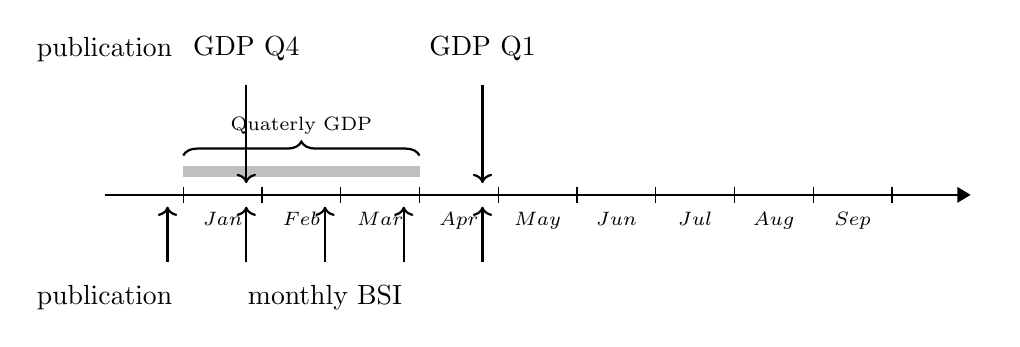
\begin{tikzpicture}
        % draw horizontal line   
        \draw[thick, -Triangle] (0,0) -- (\ImageWidth,0) node[font=\scriptsize,below left=3pt and -8pt]{ };
        % draw vertical lines
        \foreach \x in {1,...,10}
        \draw (\x cm,3pt) -- (\x cm,-3pt);
        \foreach \x/\descr in {1.5/Jan, 2.5/Feb, 3.5/Mar, 4.5/Apr, 5.5/May, 6.5/Jun, 7.5/Jul, 8.5/Aug,9.5/Sep}
        \node[font=\scriptsize, text height=1.75ex,
        text depth=.5ex] at (\x,-.3) {$\descr$};
        % colored bar up
        \foreach \x/\perccol in
        {1/100,2/75,3/25}
        \draw[lightgray, line width=4pt] 
        (\x,.3) -- +(1,0);
        % braces
        \draw [thick ,decorate,decoration={brace,amplitude=5pt}] (1,0.5)  -- +(3,0) 
               node [black,midway,above=4pt, font=\scriptsize] {Quaterly GDP};
        %\draw [thick,decorate,decoration={brace,amplitude=5pt}] (6,-.9) -- +(-1,0)
        %       node [black,midway,font=\scriptsize, below=4pt] {Publication};
        % time of publication
        \node[align=center] at (0,1.85) {publication};
        \node[align=center] at (1.8,1.85) {GDP Q4};
        \draw [thick,->] (1.8,1.4) -- (1.8,0.15);
        \node[align=center] at (4.8,1.85) {GDP Q1};
        \draw [thick,->] (4.8,1.4) -- (4.8,0.15);
        \node[align=center] at (2.8,-1.3) {monthly BSI};
        \node[align=center] at (0,-1.3) {publication};
        \draw [thick,->] (0.8,-0.85) -- (0.8,-0.15);
        \draw [thick,->] (1.8,-0.85) -- (1.8,-0.15);
        \draw [thick,->] (2.8,-0.85) -- (2.8,-0.15);
        \draw [thick,->] (3.8,-0.85) -- (3.8,-0.15);
        \draw [thick,->] (4.8,-0.85) -- (4.8,-0.15);
    \end{tikzpicture}
    \caption{Timeline of the period and the publication of the business survey indicator (BSI) and the Gross Domestic Product (GDP)}
    \label{fig:timeline}
\end{figure}

Nowcasting became a catch-all word and includes a variety of predictive models as Linear regression, ARIMA models, State-Space models, Mixed-data sampling (MIDAS) regressions, Autoregressive Distributed Lag (ARDL) models  and much more.

A good example of nowcasting is the model explained in \cite{de_antonio_liedo_nowcasting_2014} which is a State-Space model developed at the NBB. It takes into account a lot of different predictive variables to predict the actual state of .................................

Indicators that can be used aside from the business survey are average weekly work hours, factory orders for goods, housing permits and stock prices index of consumer expectations, average weekly claims for unemployment insurance and the interest rate and more.


\subsection{Business Cycles}
\label{sec:Business Cycles}

In 1946, \citeauthor{mitchell_measuring_1946} defined a business cycle as a recursive fluctuations, affecting macroeconomics variables. Since then a lot of variables where used to model business cycles but it's commonly admitted that Growth Domestic Product (GDP) is the most important of them. 
A good measure of the growth of GDP is year on year GDP that is obtained as follow

\begin{eqnarray}
   \mbox{YoY GDP} = \frac{\mbox{GDP}_t - \mbox{GDP}_{t-12}}{\mbox{GDP}_{t-12}}      \label{eq:YoY GDP}
\end{eqnarray}


\autoref{fig:Business Cycle} shows a simplified version of business cycles theory when using as measure GDP or YoY GDP.

\begin{figure}[htp!]
     \centering \footnotesize
    \small
    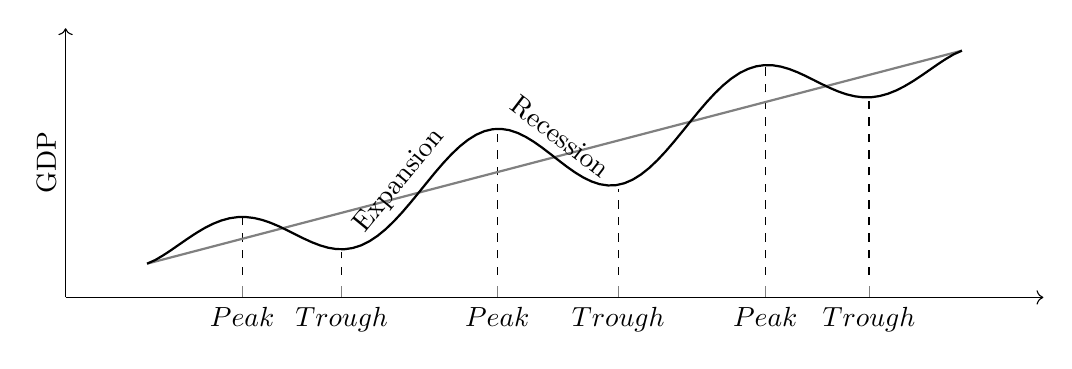
\begin{tikzpicture}
        \begin{axis}[
            domain=0:6*pi,
            samples=100,
            axis lines*=left, 
            axis line style={->},
            xtick={2.2, 4.5, 8.1, 10.9, 14.3, 16.7}, ytick=\empty,
            xticklabels = {$Peak$, $Trough$, $Peak$, $Trough$, $Peak$, $Trough$},
            width=14cm, height=5cm,
        %    xlabel={time}, 
            ylabel={GDP}
        ]       
        \addplot[mark=none, dashed] coordinates {(2.2, -1) (2.2, 4)};
        \addplot[mark=none, dashed] coordinates {(4.5, -1) (4.5, 1)}; 
        \addplot[mark=none, dashed] coordinates {(8.1, -1) (8.1, 12)}; 
        \addplot[mark=none, dashed] coordinates {(10.9, -1) (10.9, 6.6)}; 
        \addplot[mark=none, dashed] coordinates {(14.3, -1) (14.3, 17.5)}; 
        \addplot[mark=none, dashed] coordinates {(16.7, -1) (16.7, 14.9)}; 
        \addplot [thick, gray] {x};
        \addplot [thick, black] {x + 4*sin(deg(x)) * sin(deg(x/6))^0.5}
        %    node [pos=0.1, anchor=south] {Peak}
            node [pos=0.3, anchor=south, sloped] {Expansion}
            node [pos=0.49, anchor=south, sloped] {Recession}
        % Add line to show end of and ... peak and ... line
        ;
        \end{axis}
    \end{tikzpicture}
        
    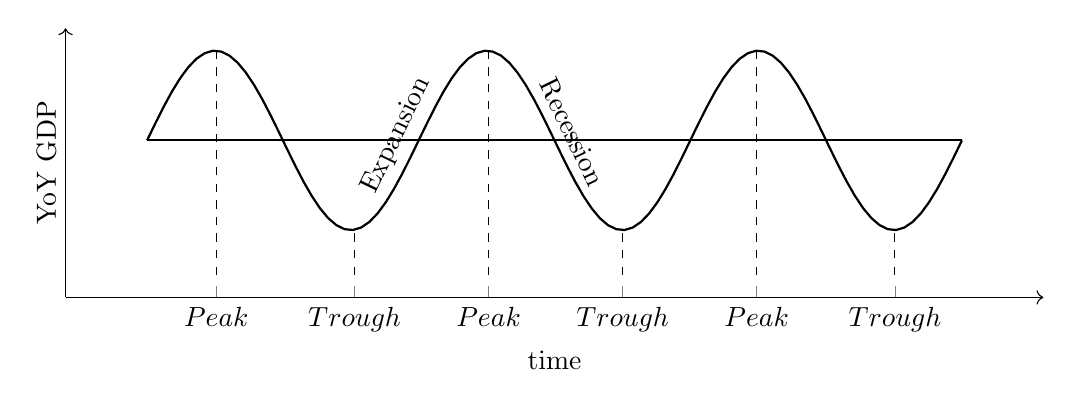
\begin{tikzpicture}
        \begin{axis}[
            domain=0:6*pi,
            samples=100,
            axis lines*=left, 
            axis line style={->},
            xtick={1.6, 4.8, 7.9, 11, 14.1, 17.3}, ytick=\empty,
            xticklabels = {$Peak$, $Trough$, $Peak$, $Trough$, $Peak$, $Trough$},
            width=14cm, height=5cm,
            xlabel={time}, 
            ylabel={YoY GDP}
        ]       
        \addplot [thick, black] {sin(deg(x))}
        %    node [pos=0.1, anchor=south] {Peak}
            node [pos=0.33, anchor=south, sloped] {Expansion}
            node [pos=0.5, anchor=south, sloped] {Recession}
        ;
        \addplot [thick, black] {0};
        \addplot[mark=none, dashed] coordinates {(1.6, -1.5) (1.6, 1)};
        \addplot[mark=none, dashed] coordinates {(4.8, -1.5) (4.8, -1)}; 
        \addplot[mark=none, dashed] coordinates {(7.9, -1.5) (7.9, 1)}; 
        \addplot[mark=none, dashed] coordinates {(11, -1.5) (11,-1)}; 
        \addplot[mark=none, dashed] coordinates {(14.1, -1.5) (14.1, 1)}; 
        \addplot[mark=none, dashed] coordinates {(17.3, -1.5) (17.3, -1)}; 
        \end{axis}
        \end{tikzpicture}
    \caption{The Business Cycle theory of GDP and year on year GDP}
    \label{fig:Business Cycle}
\end{figure}


A very important question considering business cycles is their duration.
\autoref{fig:Business Cycle} can give the false impression that business cycles are all of the same lengths, this is, in real life, not so simple.

Probably the first person to explore the duration of a business cycle was a French statistician,  \cite{juglar_crises_1862}, who set the business cycles to have a duration of 7 to 11 years.
\cite{mitchell_measuring_1946} proposed a minimum duration of 16-22 months and a maximum duration of 100-106 months.
Lot of other propositions where done even though business cycles are rather empirically defined than theory based.
Therefore let put the theory aside and look into real data.
The example of the United States is interesting since the National Bureau of Economic Research (NBER) dated precisely and methodologically the turning points for the American economy. The empirical evidence that comes out of this work, is that the time from one economic peak to the next is on average 5 and a half years for the period 1945-2009.

We can see from \autoref{fig:NBER BS}, which represent the different bottoms and peaks of business cycles identified by the NBER from 1975 to 2009, that there is no symmetry of the business cycles. Some business cycles are very short while others last more than ten years.
We can notice that periods of economic growth, usually last longer than economical decrease.

\begin{figure}[H]
     \centering \footnotesize
    \small
    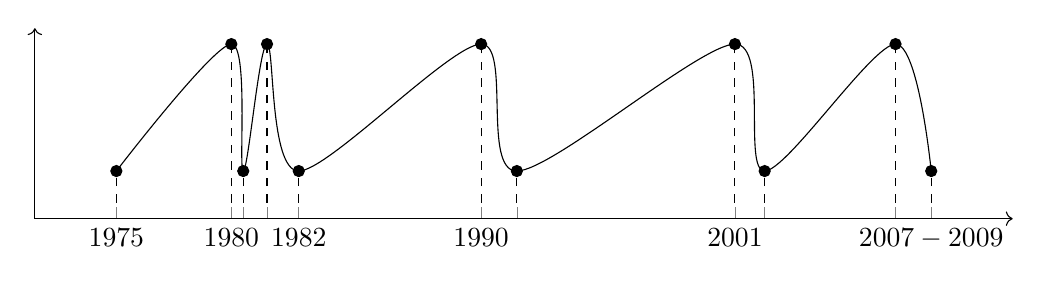
\begin{tikzpicture}
        \begin{axis}[
            domain=0:6*pi,
            samples=100,
            axis lines*=left, 
            axis line style={->},
            xtick={2103, 2161, 2167, 2179, 2195, 2287, 2305, 2415,2430, 2496, 2514}, ytick=\empty,
            xticklabels = {$1975$, $1980$,  , , $1982$, $1990$, , $2001$, , ,$2007-2009$},
            width=14cm, height=4cm
        %    xlabel={time} 
        %    ylabel={YoY GDP}
        ]       
            \addplot[smooth, mark=*,black] plot coordinates {
            (2103,-1)
            (2161,1)    (2167,-1)
            (2179,1)    (2195,-1)
            (2287,1)    (2305,-1)
            (2415,1)    (2430,-1)
            (2496,1)    (2514,-1)
            };
        \addplot[mark=none, dashed] coordinates {(2103, -1.5) (2103, -1)};
        \addplot[mark=none, dashed] coordinates {(2161, -1.5) (2161, 1)}; 
        \addplot[mark=none, dashed] coordinates {(2167, -1.5) (2167, -1)}; 
        \addplot[mark=none, dashed] coordinates {(2179, -1.5) (2179, 1)}; 
        \addplot[mark=none, dashed] coordinates {(2195, -1.5) (2195,-1)}; 
        \addplot[mark=none, dashed] coordinates {(2287, -1.5) (2287, 1)}; 
        \addplot[mark=none, dashed] coordinates {(2305, -1.5) (2305,-1)}; 
        \addplot[mark=none, dashed] coordinates {(2415, -1.5) (2415, 1)}; 
        \addplot[mark=none, dashed] coordinates {(2430, -1.5) (2430, -1)}; 
        \addplot[mark=none, dashed] coordinates {(2496, -1.5) (2496, 1)}; 
        \addplot[mark=none, dashed] coordinates {(2514, -1.5) (2514, -1)}; 
        \end{axis}
    \end{tikzpicture}
      \caption[Caption for LOF]{Business cycles from 1975 to 2009 of the American Economy according to the NBER\footnotemark}
    \label{fig:NBER BS}
\end{figure}

\footnotetext{data available at \url{https://www.nber.org/cycles.html}}

\section{Methodology of the Business Survey}
\label{section:Methodology}

%The latest large improvement of the business survey is explained in detail in \textit{"The National Bank of Belgium’s new business survey indicator"} (\citeauthor{de_greef_national_2009}).

Since 65 years of existence, the business survey was able to evolve without losing in long term comparability.

Three main methodology revisions since the launch of the business survey, in 1983, 1990 and 2009 (see \cite{de_greef_national_2009}).
The most significant changes brought in 2009 where the number of questions taken into the calculation of the BSI, which was reduced to 3-4 questions, depending on the sector, for more simplicity and accuracy.
Other improvements where the inclusion of the sector of services in the calculation of the global indicator and a new, simple method of smoothing the indicator.

\subsection{Sampling Method}
\label{sec:Recruitment of participants}

The Belgian business survey - as most of the business surveys around the world - has the particularity of not using random sampling. 
The selection of participants is quite complex and a lot of decisions are human, never is a statistical program or a random sampling system used to select new participants.
Reasons 
-> volutary basis
-> Panel data with high involvement


The selection of new participants is done by waves. When the department responsible for the business survey at the NBB decides that there aren't enough participants in a specific sector anymore, the recruitment of new participants is launched.

To find the new respondents, the first step is to decide for an optimal amount of new participants needed, regarding the different stratification of the sector.
Each sector is composed of quite advanced trees of sub-sectors, sub-sub-sectors,  and more. For example, the industry sector is divided into more than 300 sub-sectors / branches over 6 different levels. 

It could be that some subdivision of a certain sector only has 1 or 2 respondents while it accounts for a significant part of the Belgian economy. The Department of the business survey of the NBB will then look into which company, from that specific part of the economy, could be a good fit as new respondent of the business survey, considering its activity, it's size, region, and other characteristics.
As will be seen in \autoref{sec:Weighting procedure} more in detail, companies are weighted by there size (profit, number of employees, ...) and the size of the sector/branch they are part of. That information is crucial for selecting new participants.
The procedure is quite complex and therefore contains a lot of human decisions.
 
Out of this process comes a list of potential new participants. This list is then sent to the Communication Department that makes contact with those potential new participants. 
Not always, but usually, a representative of the National Bank visits the new participant to explain the survey and have a contact.
As a reward for participating in the survey, the companies receive privileged information. Each month they receive access to sub-sector indicators information that aren't publicly distributed. This can give them economical information regarding their specific sector of economic activity.

At the National Bank of Belgium, this procedure is usually referred to as prospecting, rather than selecting or sampling, since it is mostly based on recruiting new companies that will work/collaborate with them. New companies can be included in the survey outside of this procedure but this happens more occasionally.


An important side of the business survey is that people are staying as long as possible in the survey.
From the moment companies are part of the survey, they stay in it until they decide to leave, there are no participants removed from the survey by the National Bank, what can happen is that if participants don't answer for three months, contact will be taken with the company to see if they want to continue to participate.

There are resources put by the National Bank to make sure companies answer to the survey, and stay in it.
This means that some companies are part of the survey for a very long time.
To have an idea, if we look at the survey for the industry and trace respondents back to 30 years ago (1989), we can see that today, approximately one-third of the respondents were already in the survey in 1988. 


From a statistical point of view, it can seem rather problematic to draw general conclusions over a population when not using random sampling.
Without undermining one of the most important pillars of statistics, there are two main reasons why in this case, having a non-random selection of participants is not truly problematic.

The first reason is that the sampling method used is trying to represent as good as possible the population that it is representing. Therefore stratification is used at a quite advanced level as explained before. 
We could call this recruitment method: non-random stratification, as opposed to random stratification. Since it's not using sampling but takes into account the stratification of the population it's studying.

The second reason, the most import one, is that the value of the business survey indicator doesn't have interest on its own. Indeed having a BSI equal to 0.5 or 0.1 doesn't mean much, what's important is the evolution of the indicator. If it was equal to 0.3 last month and this month it's equal to 0.5, it means that the economy is most probably growing and that we can forecast an increase of GDP over the month. On the other hand, if it's now equal to 0.1, it means a decrease in economic confidence among businesses and we can anticipate a deceleration or decline of the economy over the month.



\subsection{Questionnaire}
\label{sec:Questionnaire}

The questionnaire exists in two languages, french and dutch (see Appendix \autopageref{Questionnaire2018}). It can be answered by mail, email, over the phone or by fax.
It is divided into two part:
(1) questions concerning current production and level of activity (\textit{"verloop en beoordeling"}) and
(2) questions concerning predictions, expectation of the level of activity over the next three months ("\textit{vooruitzichten voor de volgende drie maanden}").

The business survey indicator is also called the confidence indicator, since its a measure of how confidence companies are in the Belgian economy.
Almost all the questions have only three possible answers that can be interpreted as a negative, neutral or positive answer.

In this paper, the answers and results of the industry business survey barometer will be used since 1988. Therefore it's very important to see if modifications were applied over time to the questionnaire.
A questionnaire from 1990 can be seen in appendix (see \autopageref{Questionnaire1990}) and can be compared to a more recent version (see appendix \autopageref{Questionnaire2018}).

The layout was modified, and the phrasing of the questions changed over this long period. It was before asked in the first person while it's now phrased in the third person. Aside from those small changes, the survey kept the same questions and order.
It would be interesting to have a closer look at the potential consequences of those changes over time. The layout, the phrasing and the method of answering can potentially influence the answers. Nevertheless, since it's not the subject of this paper, we will leave this study to future research.
What we can say, is that the influence of those changes could be limited since the respondents where mostly the same when the changes happened, so the interpretation they made from the questions could have a smaller impact.

The interest of this paper is the industry business survey indicator, which takes four questions into account (questions 18, 27, 32 and 33). The questions are translated into English on \autopageref{Appendix: Question NS975 description} and are renumbered from 1 to 4 for simplicity.
The two first questions relate to the current state of the company while the two others ask the participants there prediction for the next three months.
The first question is about the stock of the company, 
the second question relates to the demand of there product, 
the third questions relate to the company's predictions of need of work forces 
and the last question ask their predictions regarding demand.


\subsection{Weighting Procedure}
\label{sec:Weighting procedure}

The different companies participating in the business survey have all two weights; (1) according to the size of the company and (2) according to the size of the sector branch which the company is part of.

The weight size is calculated based on the profit the company is making, the capital it's owning, the number of employees and other characteristics. 
The calculation is quite complex and is specific to each sector. 
For example, the companies having an industrial activity have a different calculation than a restaurant or a financial services company.

Since the characteristics taken into account during the calculation of the weight of each company aren't fixed, the weight of the companies is corrected periodically. 
Ones the new weight is calculated, the transition between the old and new weight is smoothened over a year.

Regarding the globalisation weighting procedure, the National Bank of Belgium developed an elaborate division of the Belgian economic activity. This means that for example, the industry is subdivided into different sub-sectors, that they self contain sub-sectors that contain sub-sectors and so on for a total of six levels. 

Each division has a percentage according to its size in the economy.
To obtain the weight of the lowest globalisation, the weight of each subdivision need to be multiply. 

The procedure of weighting is then as follow

\begin{eqnarray}
    \omega_i = \frac{ \text{weight company $i$} }{ \sum\text{company weights within globalisation} } * \text{globalisation weight} \\ \nonumber
\end{eqnarray}

where $\sum_{i=1}^{n} \omega_i = 1 $. In other words, the specific weight for each company taking the two weighting procedures into account ($\omega_i$), is obtained by dividing its weight coefficient by the total of weight coefficients within the lowest level of globalisation and multiply it with the weight of globalisation it's part of. 


\section{Calculation of the Indicator}

This section presents the method of calculation of the business survey indicator.
The calculation in itself is rather standard, but the different ways to write it are important for the interpretation and a better understanding of the indicator and the following chapters.
We first present the calculation taking into account one question unweighted and then weighted. 
After we will present how different questions are combined together to obtain a business survey indicator.


\subsection{Unweighted Indicator}

The calculation of the unweighted indicator for a specific question at a specific time is the mean of the responses and can be written as follow;

\begin{equation}
    E(X) = \frac{ \sum_{i=1}^n x_i}{n}
\end{equation} 

where 
$x_i$ is the answer of the respondent $i$ and can take value $-1$ (negative answer), $0$ (neutral answer) and $1$ (positive answer). 
$n$ is the number of respondents.

Since $x_i$ can only take three different values, we can decompose it into 

\begin{equation}
    E(X) = \frac{ \sum_{i=1}^{n_+} x_{+i} + \sum_{i=1}^{n_0} x_{0i} + \sum_{i=1}^{n_-} x_{-i}}{n}
\end{equation} 


where 
$x_{+i}$, $x_{0i}$ and $x_{-i}$ are the positive (+), neutral (N) and negative (-) answers of the respondent $i$.

Since we know that $\sum_{i=1}^n x_{0i} = 0$, we can write

\begin{equation}
    E(X) = \frac{\sum_{i=1}^{n_+} x_{+i}}{n}  + \frac{\sum_{i=1}^{n_-} x_{-i}}{n}
\end{equation} 

${\sum_{i=1}^n x_{+i}}/{n}$ is the proportion of positive answers and ${\sum_{i=1}^n x_{-i}}/{n}$ is the negative proportion of negative answer. We can write, for simplicity

\begin{equation}
    E(X) = \pi_+ - \pi_-  \label{eq: BSI Unweighted}
\end{equation}

where $\pi_+$ and $\pi_-$ are the proportion of respondents answering positive and negative to the specific question.
$\pi$ was chosen as a symbol here since it can be interpreted as a probability: if we assume that all the respondents have the same probability of giving a certain answer, $\pi$ is the probability that a respondent answers positive, negative or neutral to the question. 


\subsection{Weighted Indicator}

As described in \autoref{sec:Weighting procedure}, each respondent has two different weights: one according to its size, one according to the size of the sector it's part of. Those weights are then combined and we end up with a specific weight $\omega_i$.
We have now the following equation for the indicator

\begin{equation}
    E(X) = \sum_{i=1}^n \omega_i x_i  \quad \text{  where  } \sum_{i=1}^n \omega_i =  1
\end{equation} 

$x_i$ is the answer of the respondent $i$ and can take values -1, 0 and 1.
$\omega_i$ is the weight of respondents $i$. 
The weights are here standardised so there sum is equal to one.

As for the unweighted indicator, we can decompose the equation by the three possible answers with, in this case, their according weights.

\begin{equation}
    E(X) = \sum_{i=1}^{n_+} \omega_{i} x_{+i} + \sum_{i=1}^{n_0} \omega_{i} x_{0i} + \sum_{i=1}^{n_-} \omega_{i} x_{-i}
 \end{equation}
and again we know that $\sum_{i=1}^n \omega_{0i} x_{0i} = 0$, so we can write

\begin{equation}
    E(X) = \sum_{i=1}^{n_+} \omega_{i} x_{+i} + \sum_{i=1}^{n_-} \omega_{i} x_{-i}
\end{equation} 
We also know that $x_{+i} = 1$  and $x_{-i}=-1$  
\begin{equation}
    E(X) = \sum_{i=1}^{n_+} \omega_{i}  - \sum_{i=1}^{n_-} \omega_{i}
\end{equation}
That we will write as follow
\begin{equation}
    E(X) = \Omega_+ - \Omega_- \label{eq: BSI Weighted}
\end{equation}

where $\Omega_+$ and $\Omega_-$ are the sum of weights of positive and negative respondents. 
In other words, $\Omega_+$ and $\Omega_-$ are the weighted proportion of respondents answering positive and negative. 

$\Omega$ is used here also in the probabilistic way as it can also be seen as the probability that a respondent answers positive, negative or neutral ($\Omega_0$) with $\Omega_+ + \Omega_0 + \Omega_- =1$. Here we speak of weighted proportions/probabilities.

From \autoref{eq: BSI Unweighted} and \autoref{eq: BSI Weighted} it can be seen that the weighted and unweighted indicators are bounded between -1 and 1. In the two cases, the indicator is the smallest if everyone has a negative answer, and is the largest when every answer is positive.

\subsection{Take Different Questions Into Account}

The previous calculations were specific to one question. The published indicators are usually taking different survey questions into account. For example, the industry indicator that we will be interested in is composed of four questions:

\begin{equation}
    \mbox{Industry BSI}\ = \frac{E(X_{Q1}) + E(X_{Q2}) + E(X_{Q3}) + E(X_{Q4})}{4}
\end{equation}

where 
$E(X_{Q1})$, $E(X_{Q2})$, $E(X_{Q3})$ and $E(X_{Q4})$ are the different averages for question 18, 27, 32 and 33 (can be weighted or unweighted).

The equation can also be written as follow for the unweighted indicator\footnote{Assuming all the respondents answered to all the questions.}


\begin{equation}
    \mbox{Unweighted Industry BSI}\ = \frac{\sum^n_{i=1}(x_{iQ1} + x_{iQ2} + x_{iQ3} + x_{iQ4})}{4n} 
\end{equation} 

\begin{equation}
    \mbox{Unweighted BSI}\ = \frac{\sum^n_{i=1}( x_{iQ1} + x_{iQ2} + \ldots + x_{iQq})}{nq} 
\end{equation} 

and as follow for the weighted indicator\footnote{Assuming all the respondents answered to all the questions and that the weighting ($\omega_i$) is the same across all the questions.}


\begin{equation}
    \mbox{Weighted Industry BSI}\ = \frac{\sum^n_{i=1} \omega_i (x_{iQ1} + x_{iQ2} + x_{iQ3} + x_{iQ4})}{4} 
\end{equation} 

\begin{equation}
    \mbox{Weighted BSI}\ = \frac{\sum^n_{i=1} \omega_i ( x_{iQ1} + x_{iQ2} +\ldots + x_{iQ4q})}{q} 
\end{equation} 


Another way to write the unweighted business survey indicator is as follow

\begin{eqnarray}
    \mbox{Unweighted industry BSI}\ &=& \Large( \pi_{Q1+} + \pi_{Q2+} + \pi_{Q3+} + \pi_{Q4+} \nonumber \\
    && - \pi_{Q1-} - \pi_{Q2-} - \pi_{Q3-} - \pi_{Q4-} \Large)
\end{eqnarray}

and regarding the weighted indicator, it can be written as

\begin{eqnarray}
    \mbox{ Weighted Industry BSI}\ &=& 1/4 ( \Omega_{Q1+} + \Omega_{Q2+} + \Omega_{Q3+} + \Omega_{Q4+} \nonumber \\
    && - \Omega_{Q1-} - \Omega_{Q2-} - \Omega_{Q3-} - \Omega_{Q4-} \Large) 
\end{eqnarray}

..........................................................;

The general formula for the weighted business survey indicator when taking several questions into account is

\begin{eqnarray}
    \mbox{ Unweighted BSI}\ &=& 1/q ( \pi_{Q1+} +  \pi_{Q2+} + \ldots +  \pi_{Qq+}  -  \pi_{Q1-} -  \pi_{Q2-} -  \pi_{Qq-} \Large) 
\end{eqnarray}

While the formula for the weighted business survey indicator when taking several questions into account is

\begin{eqnarray}
    \mbox{ Weighted BSI}\ &=& 1/n ( \pi_{Q1+} + \Omega_{Q2+} + \ldots + \Omega_{Qq+} - \Omega_{Q1-} - \Omega_{Q2-} - \ldots - \Omega_{Qq-} \Large) \nonumber\\
\end{eqnarray}




\chapter{The Variance of the Indicator}

The variance is, with the mean, one of the first tool for statisticians to study a certain variable. 
Next, to the mean, that is the average value of a certain variable, the variance is the measure of the dispersion. 
In the context of the business survey, the variance can be seen as "how much companies (dis)agree on the present state of the Belgian economy", a piece of important information that we can extract from the survey.

% A small comment can be written regarding the difference between the variance and sampling error. The idea here is not the study accuracy or ... but rather to find new information hidden in the survey.

This chapter will present the calculation of the variance of the unweighted and weighted indicator for one question of the business survey. It will then be looked into its properties and specificities.
The last section will present the method of calculation when different questions are taken into account.

\section{Variance of the Unweighted Indicator}

\nocite{alcaniz_calculation_2006}

The formula of the variance can be written as 
\begin{eqnarray}
         \Var(X) &=& E \left[ \left(X-E(X) \right)^2 \right] =  E\left( X^2\right) - E\left( X\right)^2
\end{eqnarray}

In the case of one question of the business survey indicator, we decompose and develop the equation as follow

\begin{eqnarray}
\Var(X) &=&  E\left( X^2\right) - E\left( X\right)^2 \nonumber \\ \nonumber \\
    &=& \left( \frac{\sum_{i=1}^{n_+} x_{+i}^2}{n} \right)  + \left( \frac{\sum_{i=1}^{n_0} x_{0i}^2}{n} \right) + \left( \frac{\sum_{i=1}^{n_-} x_{-i}^2}{n} \right) - E(X)^2 \\ \nonumber 
\end{eqnarray}


Since the positive answers take value 1 and negative answers value -1 ($x_{+i}^2 = x_{+i} = 1$ and $x_{-i}^2 = |x_{-i}| = 1$), and $\left( \frac{\sum_{i=1}^{n_0} x_{0i}^2}{n} \right) = 0$. 
The equation can further be simplified to

\begin{eqnarray}
    \Var(X) &=& \pi_+ + \pi_- - E ( X )^2 \label{var1} \\ \nonumber
\end{eqnarray}

Where $\pi_+$ and $\pi_-$ are the proportions of positive and negative answers.

In other words, the variance of the BSI is equal to the sum of the proportion of positive and negative answers, minus the squared indicator.

Since $\E(X)=\pi_+ - \pi_-$, and $\pi_+ + \pi_- = 1 - \pi_0$ (from $\pi_+ + \pi_0 + \pi_- = 1$).
It's possible to write the variance in several different ways;

%We can also replace $\E(X)$  by $\pi_+ - \pi_-$, and/or $\pi_+ + \pi_-$ by $ 1 - \pi_0$ (since $\pi_+ \pi_0 + \pi_- = 1$). Which means that we have several different ways to write the previous equation;

\begin{eqnarray}
\Var(X) &=& \pi_+ + \pi_- - E ( X )^2  \nonumber \\
        &=& \pi_+ + \pi_- - ( \pi_+ - \pi_- )^2 \label{eq:var2} \\
        &=& 1 - \pi_0 - E(X)^2 \label{eq:var3}
\end{eqnarray}




\section{Variance of the Weighted Indicator}

We can now do the same for the weighted indicator. The equation is very similar to the variance of the unweighted variance;



\begin{eqnarray}
\Var(X) &=&  E\left( X^2\right) - E\left( X\right)^2 \nonumber \\ \nonumber \\
    &=& \sum_{i=1}^{n_+} \omega_i x_{+i}^2 + \sum_{i=1}^{n_0} \omega_i x_{0i}^2  + \sum_{i=1}^{n_-} \omega_i x_{-i}^2 - E(X)^2 \nonumber \\
\end{eqnarray}

As we did for the indicator, we will develop the equation by taking into account weighted proportion and write the equation the same way as for the unweighted variance. 
Again the variance can be written in different ways;

\begin{eqnarray}
\Var(X) &=& \Omega_+ + \Omega_- - ( \Omega_+ - \Omega_- )^2 \\
    &=& \Omega_+ + \Omega_- - E ( X )^2 \\
    &=& 1 - \Omega_{0} - E(X)^2 \label{eq:var3 weighted}
\end{eqnarray}


\section{Properties}
    \label{sec:properties variance}

\begin{figure}[hbt!]
     \centering \footnotesize
    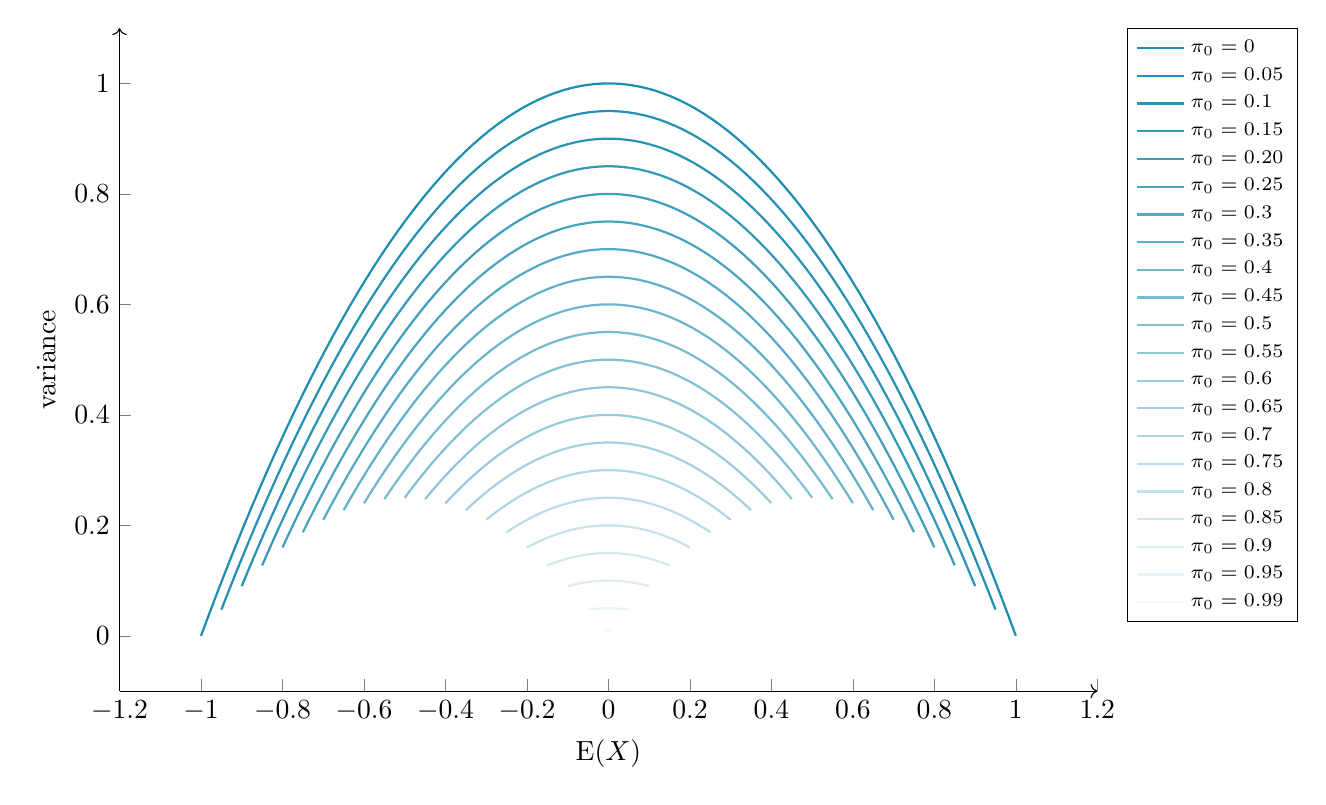
\begin{tikzpicture}
    \tikzset{
      legendmatrix/.style={% style for legends
        draw,% draw a border for the legend
        outer sep=.3333em,% additional space to the axis label
        nodes={rotate=90,anchor=base west,outer sep=0pt},% rotate the nodes inside the matrix
        /pgfplots/every crossref picture/.append style={yshift=.75ex}% rotate the legend images
      }
    }
    \begin{axis}[
        domain=-1:1,
        samples=100,
        axis lines*=left, 
        axis line style={->},
        width=14cm, height=10cm,
        xlabel={$\E(X)$}, ylabel={variance},
    legend pos= outer north east, legend cell align=left,
     legend style={font=\scriptsize}
     ]       
    \addplot [thick, bluetitle!100, domain = -1:1] {1 - x^2};
    \addplot [thick, bluetitle!97, domain = -0.95:0.95] {1 - 0.05 - x^2};
    \addplot [thick, bluetitle!95, domain = -0.9:0.9] {1 - 0.1 - x^2};
    \addplot [thick, bluetitle!90, domain = -0.85:0.85] {1 - 0.15 - x^2};
    \addplot [thick, bluetitle!85, domain = -0.8:0.8] {1 - 0.2 - x^2};
    \addplot [thick, bluetitle!80, domain = -0.75:0.75] {1 - 0.25 - x^2};
    \addplot [thick, bluetitle!75, domain = -0.7:0.7] {1 - 0.3 - x^2};
    \addplot [thick, bluetitle!70, domain = -0.65:0.65] {1 - 0.35 - x^2};
    \addplot [thick, bluetitle!65, domain = -0.6:0.6] {1 - 0.4 - x^2};
    \addplot [thick, bluetitle!60, domain = -0.55:0.55] {1 - 0.45 - x^2};
    \addplot [thick, bluetitle!55, domain = -0.5:0.5] {1 - 0.5 - x^2};
    \addplot [thick, bluetitle!50, domain = -0.45:0.45] {1 - 0.55 - x^2};
    \addplot [thick, bluetitle!45, domain = -0.4:0.4] {1 - 0.6 - x^2};
    \addplot [thick, bluetitle!40, domain = -0.35:0.35] {1 - 0.65 - x^2};
    \addplot [thick, bluetitle!35, domain = -0.3:0.3] {1 - 0.7 - x^2};
    \addplot [thick, bluetitle!30, domain = -0.25:0.25] {1 - 0.75 - x^2};
    \addplot [thick, bluetitle!25, domain = -0.2:0.2] {1 - 0.8 - x^2};
    \addplot [thick, bluetitle!20, domain = -0.15:0.15] {1 - 0.85 - x^2};
    \addplot [thick, bluetitle!15, domain = -0.1:0.1] {1 - 0.9 - x^2};
    \addplot [thick, bluetitle!10, domain = -0.05:0.05] {1 - 0.95 - x^2};
    \addplot [thick, bluetitle!05, domain = -0.01:0.01] {1 - 0.99 - x^2};
 %    \addplot [thick, black, domain = -1:0] { - ((x+0.5)^2) + 0.25};
 %    \addplot [thick, black, domain = 0:1] { - ((x-0.5)^2) + 0.25};
%     \addplot [thick, black, domain = -1:0] {-x-x^2};
%     \addplot [thick, black, domain = 0:1] {x-x^2};
%     \addplot [thick, black, domain = -1:1] {(x^2)*(-y)-(y^2)/2 + y};    
    \addlegendentry{$\pi_0 = 0$}
    \addlegendentry{$\pi_0 = 0.05$}
    \addlegendentry{$\pi_0 = 0.1$}
    \addlegendentry{$\pi_0 = 0.15$}
    \addlegendentry{$\pi_0 = 0.20$}
    \addlegendentry{$\pi_0 = 0.25$}
    \addlegendentry{$\pi_0 = 0.3$}
    \addlegendentry{$\pi_0 = 0.35$}
    \addlegendentry{$\pi_0 = 0.4$}
    \addlegendentry{$\pi_0 = 0.45$}
    \addlegendentry{$\pi_0 = 0.5$}
    \addlegendentry{$\pi_0 = 0.55$}
    \addlegendentry{$\pi_0 = 0.6$}
    \addlegendentry{$\pi_0 = 0.65$}
    \addlegendentry{$\pi_0 = 0.7$}
    \addlegendentry{$\pi_0 = 0.75$}
    \addlegendentry{$\pi_0 = 0.8$}
    \addlegendentry{$\pi_0 = 0.85$}
    \addlegendentry{$\pi_0 = 0.9$}
    \addlegendentry{$\pi_0 = 0.95$}
    \addlegendentry{$\pi_0 = 0.99$}
    \end{axis}
    \end{tikzpicture}
    \caption{Plot of the possible values of the indicator (X axis) and variance (Y axis) for different values of $\pi_0$ }
    \label{fig:var properties}
\end{figure}


Based on the previous development of the equation of the variance of the indicator, we can make some observations.

First of all, the variance is bounded between 0 and 1. 
A variance can't be negative since it's a sum of squares, so the lower bound shouldn't surprise anyone. On the other hand, the upper bound is more unusual. 
An interesting approach is to take  \autoref{eq:var3} and see that $\pi_0$ and $\E(X)^2$ can only take positive values, $\pi_0$ because it's a proportion and $\E(X)^2$ since it's squared. 
Both variables have a minus sign in the equation, so the highest results are obtained when both variables are equal to zero.
In other words, the highest variance is obtained when no respondent answer "neutral" and the BSI is equal to 0. 
This happens when their are as much negative as positive answers (50-50).
This corresponds to the interpretation described before, since it's the situation with the most disagreement among respondents.
In the other hand, if all participants answer the same ("negative", "neutral" or "positive"), the variance is equal to zero.
It corresponds to the situation where the agreement among respondents is the highest.

Another approach to better understand the variance of the business survey barometer, is to plot the different possible values of $\Var(X)$, $\pi_0$ and $\E(X)$ from \autoref{eq:var3} or \autoref{eq:var3 weighted}. The results can be seen in \autoref{fig:var properties}.
It's interesting to see from the plot that each $\E(X)$ can only have a certain amount of possible variance, in other words, there is a specific upper and lower bound for each indicator. For example an indicator of 0.5 can only have a variance between 0.25 and 0.75.
It's also interesting to notice that to know that with two of the three variables ($\Var(X)$, $\pi_0$ and $\E(X)$), it's very easy to calculate the third. This means that the three variables are related.

\section{Take Different Questions Into Account}

As already seen, the published indicator take different questions into account. 
The combination of the variance of different questions is slightly more complex than the combination of different indicators since the questions are correlated, which means that covariance has to be taken into account.

The formula to combine different variances is the following

\begin{equation}
\Var \left(\sum_{i=1}^{q} X_{i}\right) = \sum_{i=1}^{q} \sum_{j=1}^{q} \Cov\left(X_{i}, X_{j}\right)
= \sum_{i=1}^{q} \Var\left(X_{i}\right)+2 \sum_{1 \leq i<j \leq q} \Cov\left(X_{i}, X_{j}\right)
\end{equation} 

In the case of combining the variances of the four different questions of the industry business survey, we have the following equation

\begin{eqnarray}
    \Var \left(\frac{X_{Q1} + X_{Q2} + X_{Q3} + X_{Q4}}{4} \right) &=& \frac{1}{16} \large[ \Var(X_{Q1}) + \Var(X_{Q2}) + \Var(X_{Q3}) + \Var(X_{Q4}) \nonumber \\
    && + 2 \Cov (X_{Q1},X_{Q2}) + 2 \Cov (X_{Q1},X_{Q3}) + 2 \Cov (X_{Q1},X_{Q4}) \nonumber \\
    &&  + 2 \Cov (X_{Q2},X_{Q3}) + 2 \Cov (X_{Q2},X_{Q4}) + 2 \Cov (X_{Q3},X_{Q4}) \large] \nonumber \\
\end{eqnarray}

The complexity of the formula encourages to rather calculate the indicator (taking all the questions into account), and then calculate the variance of that indicator. It can be written as follow

\begin{eqnarray}
    \Var \left(\frac{X_{Q1} + X_{Q2} + X_{Q3} + X_{Q4}}{4} \right) 
    &=& \frac{1}{16} \Var \left(\frac{\sum_{i=1}^n \left(x_{i Q1} + x_{i Q2} + x_{i Q3} + x_{i Q4} \right)}{n} \right) \nonumber \\
    &=& \frac{1}{16} \Var \Large(\pi_{Q1+} + \pi_{Q2+} + \pi_{Q3+} + \pi_{Q4+} - \pi_{Q1-} \nonumber \\
&& - \pi_{Q2-} - \pi_{Q3-} - \pi_{Q4-}  \Large) 
 %   &=& \frac{1}{16} \Var \left(\pi_{1+} + \pi_{2+} + \pi_{3+} + \pi_{4+} - \pi_{1-} - \pi_{2-} - \pi_{3-} - \pi_{4-} \right) \nonumber \\
\end{eqnarray}

The generalisation of the previous equation can be written as follow for the variance of the unweighted indicator

\begin{eqnarray}
    \Var \left(\text{Unweighted BSI} \right) 
    &=& \frac{1}{q^2} \Var \left(\frac{\sum_{i=1}^n \left( x_{i Q1} + x_{i Q2} + ... + x_{i Qq} \right)}{n} \right) \nonumber \\
    &=& \frac{1}{q^2} \Var \left(\pi_{Q1+} + \pi_{Q2+} + \ldots + \pi_{Qq+} - \pi_{Q1-} - \pi_{Q2-} - \ldots - \pi_{Qq-} \right) \nonumber \\
\end{eqnarray}

and as follow for the variance of the weighted indicator

\begin{eqnarray}
    \Var \left(\text{Weighted BSI} \right) 
    &=& \frac{1}{q^2} \Var \left( \sum_{i=1}^n \omega_i \left(x_{i Q1} + x_{i Q2} + ... + x_{i Qq} \right) \right) \nonumber \\
    &=& \frac{1}{q^2} \Var \Large(\Omega_{Q1+} + \Omega_{Q2+} + \ldots + \Omega_{Qq+} \nonumber \\
    && - \Omega_{Q1-} - \Omega_{Q2-} - \ldots - \Omega_{Qq-} \Large)
\end{eqnarray}




\chapter{The Indicator of the Evolution of Individual Responses}

In the same logic as for the variance, a proposition is done here of a method to extract more information out of the business survey. 
As explained in the first chapter, the business survey is answered by the same companies over time. Some new participants join and some companies leaving the survey, but the survey can be referred to and treated as a panel survey.

Is it possible to have more information by taking the evolution of the individual respondents into account? 
This chapter will address this question by applying a method proposed by \cite{caron_estimation_1996} that, by taking all the individual evolution of responses into account, offers a method to calculate an indicator that will be referred to as the indicator of the evolution of individual responses (EIR).

% We will here describe and develop this indicator, that we will call Evolution of individual Responses (EIR).
% It can be understood as the indicator of the changes in individual answers between t-1 and t.

When only one period is taken into account, there are three possible answers; "negative", "neutral" and "positive".
When we take two periods into account, a month (t) and the previous one (t-1) for example, there are nine possible situations as represented in \autoref{tab:EIR explanation}. 


\begin{table}[htp!]
     \centering \footnotesize
    \begin{tabular}{r | r | c c c | }
    \multicolumn{1}{r}{} & \multicolumn{1}{r}{} &    \multicolumn{3}{c}{$t$} \\ \cline{3-5}
    \multicolumn{1}{r}{} &         & \textbf{-} & \textbf{0} & \textbf{+} \\ \cline{2-5}
          &    \textbf{-} & $z_{i--}$    & $z_{i-0}$    & $z_{i-+}$ \\ 
    $t-1$ & \textbf{0}  & $z_{i0-}$    & $z_{i00}$    & $z_{i0+}$ \\
          &    \textbf{+} & $z_{i+-}$    & $z_{i+0}$    & $z_{i++}$ \\ \cline{2-5}
    \end{tabular}
    \caption{Possible observations when taking t and t-1 into account}
    \label{tab:EIR explanation}
\end{table}

The same as for the business survey indicator, the evolution of individual responses take different values. In the case of the BSI, $x_i$ can take value -1, 0 and 1. In the case of the EIR, $z_i$ can take values -2, -1, 0, 1 and 2.

The EIR defers also from the BSI in the sense that it's a measure of change, so if the answer of a certain respondent is the same at a certain time and the previous answer, $z_i=0$. 
% What's measured here is the difference in the answer.
On the other hand, if a certain participant changes his answer for a more positive answer it will take value 1, except if it's a radical change from a "negative" to a "positive" answer, then it will take value 2.
Same the other way around, if it decreases it will take value -1, except for a radical change from "positive" to "negative".
We will here use $z$ rather than $x$ to make a clear distinction between the BSI and the EIR.

The calculation of $z_i$ is the difference of $x_i$ at t-1 and $x_i$ at t

\begin{equation}
    z_i = x_{i,t-1} - x_{i,t}
\end{equation}

the different possible values of $z_i$ can be seen in \autoref{tab:values EIR}. 

\begin{table}[H]
     \centering \footnotesize
    \begin{tabular}{r | r | c c c | }
    \multicolumn{1}{r}{} & \multicolumn{1}{r}{} &    \multicolumn{3}{c}{$t$} \\ \cline{3-5}
    \multicolumn{1}{r}{} &         & \textbf{-} & \textbf{0} & \textbf{+} \\ \cline{2-5}
           &    \textbf{-} & $z_{i--}=0$    & $z_{i-0}=1$    & $z_{i-+}=2$ \\ 
    $t-1$ & \textbf{0}  & $z_{i0-}=-1$    & $z_{i00}=0$    & $z_{i0+}=1$    \\
            & \textbf{+}& $z_{i+-}=-2$    & $z_{i+0}=-1$    & $z_{i++}=0$ \\ \cline{2-5}
\end{tabular}
    \caption{Values of the different observations of $z_i$}
    \label{tab:values EIR}
\end{table}{}

\section{Indicator of the Unweighted Evolution of Individual Responses}

% \begin{equation}
%    \pi_{++} + \pi_{+0} + \pi_{+-} + \pi_{0+} + \pi_{00} + \pi_{0-} + \pi_{-+} + \pi_{-0} + \pi_{--} = 1
% \end{equation}

The indicator of the evolution of the individual responses can be obtained by taking the mean of the values, as defined in \autoref{tab:values EIR}, the formula is then

\begin{eqnarray}
    \E(Z) &=&  \frac{ \sum_{i=1}^n z_i}{n} \\ \nonumber \\
        &=& \left( \frac{ \sum_{i=1}^{n_{--}} z_{--i}}{n} \right)
     + \left( \frac{\sum_{i=1}^{n_{-0}} z_{-0i} }{n} \right)
    + \left( \frac{\sum_{i=1}^{n_{-+}} z_{-+i}}{n} \right)
    + \left( \frac{\sum_{i=1}^{n_{0-}} z_{0-i} }{n} \right)
    + \left( \frac{\sum_{i=1}^{n_{00}} z_{00i} }{n} \right) \nonumber  \\
    &&  + \left( \frac{\sum_{i=1}^{n_{0+}} z_{0+i}}{n} \right)
    + \left( \frac{\sum_{i=1}^{n_{+-}} z_{+-i} }{n} \right)
    + \left( \frac{\sum_{i=1}^{n_{+0}} z_{+0i} }{n} \right)
    + \left( \frac{\sum_{i=1}^{n_{++}} z_{++i}}{n} \right)
\end{eqnarray}

The formula can further be simplified since $z_{--} = z_{00} = z_{++} = 0$).

\begin{eqnarray}
    \E(Z) &=&  
     \left( \frac{\sum_{i=1}^{n_{-0}} z_{-0i} }{n} \right)
    + \left( \frac{\sum_{i=1}^{n_{-+}} z_{-+i}}{n} \right)
    + \left( \frac{\sum_{i=1}^{n_{0-}} z_{0-i} }{n} \right)
    + \left( \frac{\sum_{i=1}^{n_{0+}} z_{0+i}}{n} \right) \nonumber \\
&&  + \left( \frac{\sum_{i=1}^{n_{+-}} z_{+-i} }{n} \right)
    + \left( \frac{\sum_{i=1}^{n_{+0}} z_{+0i} }{n} \right)
\end{eqnarray}




As for the indicator, it's possible here to have a formula with proportions.

% The EIR can now be calculated with the following expression after taking out $\pi_{--}$, $\pi_{00}$ and $\pi_{++}$ (since $z_{--} = z_{00} = z_{++} = 0$).

\begin{equation}
    \E(Z) = \pi_{0+} + \pi_{-0} - \pi_{+0} - \pi_{0-} +2\pi_{-+} -2\pi_{+-} \label{eq:unweighted proprotion EIR}
\end{equation}

where $\pi$ is the proportion/probability of respondent answering negative(-), neutral (0) and positive (+) at $t-1$ and $t$. 

\autoref{eq:unweighted proprotion EIR} ...................

\section{Indicator of the Weighted Evolution of Individual Responses}

\begin{eqnarray}
    \E(Z) &=&  \sum_{i=1}^n \omega_i z_i \\ \nonumber \\
        &=& \sum_{i=1}^{n_{--}} \omega_i z_{--i} 
     + \sum_{i=1}^{n_{-0}} \omega_i z_{-0i}  
    + \sum_{i=1}^{n_{-+}} \omega_i z_{-+i} 
    + \sum_{i=1}^{n_{0-}} \omega_i z_{0-i}  
    + \sum_{i=1}^{n_{00}} \omega_i z_{00i}   \nonumber  \\
    &&  + \sum_{i=1}^{n_{0+}} \omega_i z_{0+i} 
    + \sum_{i=1}^{n_{+-}} \omega_i z_{+-i} 
    + \sum_{i=1}^{n_{+0}} \omega_i z_{+0i} 
    + \sum_{i=1}^{n_{+-}} \omega_i z_{++i} \\
&=&  \sum_{i=1}^{n_{-0}} \omega_i  
    + 2 \sum_{i=1}^{n_{-+}} \omega_i  
    - \sum_{i=1}^{n_{0-}} \omega_i         
    + \sum_{i=1}^{n_{0+}} \omega_i  
    - 2 \sum_{i=1}^{n_{+-}} \omega_i 
    - \sum_{i=1}^{n_{+0}} - \omega_i  
\end{eqnarray}


The weighted EIR can, as for the unweighted EIR now be calculated with the following expression 

\begin{equation}
    \E(Z) = \Omega_{0+} + \Omega_{-0} - \Omega_{+0} - \Omega_{0-} +2\Omega_{-+} -2\Omega_{+-} \label{eq:weighted proprotion EIR}
\end{equation}


\section{Generalisation for Different Period Lags}

Changes in the economy are usually taking several months to influence all the companies. There can be some lag of effects on for example larger companies, of a very specific sector.
The idea of only taking a certain month and the previous month can seem non-sufficient, it's relevant to take a larger period into account. 

Different methods were explored to take more than two periods into account, but it was found to be flawed and very complex to interpret.
We rather propose here a simple generalisation; use t-n rather than t-1. 
The answer at t-n are compared with the answer at time t, without taking the between answers into account.

The calculation is then the same for the unweighted as \autoref{eq:unweighted proprotion EIR} and for the weighted as \autoref{eq:weighted proprotion EIR}.


\section{Take Different Questions Into Account}


\begin{equation}
    \mbox{Industry evolution of individual responses}\ = \frac{\sum_{i=1}^n \left(z_{i Q1} + z_{i Q2} + z_{i Q3} + z_{i Q4} \right)}{4n}
\end{equation}





\subsubsection{weighted}

\begin{equation}
    \mbox{Weighted Industry EIR}\ = \frac{ \sum_{i=1}^n \omega_i \left(z_{i Q1} + z_{i Q2} + z_{i Q3} + z_{i Q4} \right)}{4}
\end{equation}


\begin{equation}
    \text{Industry evolution of individual responses} = \Omega_{0+} + \Omega_{-0} - \Omega_{+0} - \Omega_{0-} +2\Omega_{-+} -2\Omega_{+-} 
\end{equation}



\begin{equation}
    \mbox{Industry BSI}\ = \frac{\pi_{Q1+} + \pi_{Q2+} + \pi_{Q3+} + \pi_{Q4+} - \pi_{Q1-} - \pi_{Q2-} - \pi_{Q3-} - \pi_{Q4-} }{4}
\end{equation}


\begin{eqnarray}
    \mbox{ Weighted Industry BSI}\ &=& 1/4 ( \Omega_{Q1+} + \Omega_{Q2+} + \Omega_{Q3+} + \Omega_{Q4+} \\
    && - \Omega_{Q1-} - \Omega_{Q2-} - \Omega_{Q3-} - \Omega_{Q4-} \Large) 
\end{eqnarray}



\chapter{The Variance of the Evolution of Individual Responses} \label{Chapter:Var Z}

The new indicator, the evolution of individual responses, also has a variance that has some interpretation interest. 
While the EIR is a measure of the direction companies changes there answer(s), the variance of the EIR can be understood as the measure of changes in answers. 
Therefore the variance of the EIR can be seen as the volatility of the indicator, in the sense that the variance of the EIR accounts for the dispersion of the difference in answers over two periods.

While the variance of the business survey indicator is the measure  of disagreement among respondents, the variance of the evolution of individual responses is the measure of different changes of respondents.

% In this case, the highest the variance of EIR, will be obtained when half of the companies went from a negative answer to a positive answer and the other half did the opposite and changed from a positive answer at time t-1 to a negative answer at time t. 

\section{Variance of the Unweighted Evolution of Individual Responses}



%\begin{equation}
%    \pi_{++} + \pi_{+0} + \pi_{+-} + \pi_{0+} + \pi_{00} + \pi_{0-} + \pi_{-+} + \pi_{-0} + \pi_{--} = 1 
%\end{equation}

\begin{eqnarray}
Var(Z) &=& \pi_{0+} + \pi_{-0} + \pi_{+0} + \pi_{0-} +4\pi_{-+} +4\pi_{+-} \nonumber \nonumber \\ 
&&    - (\pi_{0+} + \pi_{-0} - \pi_{+0} - \pi_{0-} +2\pi_{-+} -2\pi_{+-})^2  \\
&=& \pi_{0+} + \pi_{-0} + \pi_{+0} + \pi_{0-} +4\pi_{-+} +4\pi_{+-} - E(Z)^2  \\
&=& 1 - \pi_{++} - \pi_{00} - \pi_{--} + 3\pi_{+-} + 3\pi_{-+} - E(Z)^2
\end{eqnarray}




\section{Variance of the Weighted Evolution of Individual Responses}


\section{Properties}

The 
quite similar to Var(BSI)


\subsubsection{Property 1: the variance of Z is bounded between 0 and ?}
upper bound:

\begin{eqnarray}
Var(Z) &=& 1 - \pi_{++} - \pi_{00} - \pi_{--} + 3\pi_{+-} + 3\pi_{-+} - E(Z)^2 \nonumber \\
	&=& 1 - 0 - 0 - 0 + 3*0.5 + 3*0.5 - 0 = 2.5 \nonumber
\end{eqnarray}


\begin{equation}
	1+ 0.5*3 + 0.5*3 - 0 = 2.5
\end{equation}

\subsubsection{Property 2: }

\section{Take Different Questions Into Account}




\chapter{Non-Response, Dropout, Attrition and Seasonal Effects}
\label{chap:nonresponse dropout}

Before modelling the data, it's important to look at the different effects that could mislead the outcome of the analysis. After exploring the data and doing a literature review, four main effects could mislead the results. Three are due to the survey and one to external effects; seasonal effects. We will first look into seasonal effects and apply a well know correction to the data to eliminate, as good as possible, the seasonal effects from the data.
It will then be looked into the three survey based issues; non-response, dropout and attrition.

As already mentioned before, for this analysis the data at hand is the unweighted indicators of the industry business survey, for the period of 1988 to 2018.

Eight variables will be used for the analysis; the business survey indicator, the variance of the BSI, the evolution of individual responses and the variance of the EIR (three variations of the EIR and its variance; taking a 1, 2 or 3 months comparison) 

\section{Seasonal Correction}
\label{sec:seasonal correction}

The National Bank, before publishing the business survey indicator, applies an X11 seasonal correction.

The literature about seasonal effects is very rich and variate. Without going too much into details, there are today two methods which are the most widely used and recommended which are X12/X13-ARIMA developed by the US Census Bureau and TRAMO/SEATS developed at the Bank of Spain. 

The Department of Research and Development of the NBB developed JDemetra+ which is recommended by the European Central Bank (ECB) and the European Statistical Office (Eurostat) for all National Statistics Institutes (NSI) of the European Union. 

JDemetra+ is used by the National Bank to apply seasonal corrections to the business survey indicator before publication. It will be used here, to test for seasonality and apply corrections to the data.

Tests for seasonality are summarised in \autoref{tab:Seasonality Tests}. The results are clear, there is seasonality for all of the variables.

\begin{table}[htp!]
    \centering \footnotesize
    \begin{tabular}{l|c|c|c|c|c|c|c|c}
\textbf{Seasonality Test} & BSI & Var(BSI) & EIR & Var(EIR) & EIR2 & Var(EIR2) & EIR3 & Var(EIR3) \\ \hline
Auto-corr. at seasonal lags& YES & YES & YES & YES & YES & YES & YES & YES \\
Friedman test       & YES   & YES & YES & YES & YES & YES & YES & YES \\
Kruskall-Wallis test & YES   & YES & YES & YES & YES & YES & YES & YES \\
Spectral peaks                  & YES   & YES & YES & ? & YES & ? & YES & YES \\
Periodogram                     & YES   & YES & YES & YES & YES & YES & YES & YES \\
Seasonal dummies                & YES   & YES & YES & YES & YES & YES & YES & YES \\
Seasonal dummies (AMI)          & YES   & YES & YES & YES & YES & YES & YES & YES \\
    \end{tabular}
    \caption{Seasonality Tests}
    \label{tab:Seasonality Tests}
\end{table}


% Further explanations can be found in appendix \autopageref{sec:test for seasonality}.

The different variables are seasonal correction using RJDemetra, the R package based on JDemetra+.
The results are plotted in \autoref{fig:seasonal ajusted rjdemetra}.

The method applied is is called "RSA0" and is the simplest X12/X13-ARIMA method for seasonal correction since it's not applying log/level, outliers and calendar corrections. 
It was chosen since it's the closes to the X11 applied by the NBB to the business survey when monthly publishing the indicators.

It's interesting here to notice here that there is no need for year on year GDP seasonal correction since  it's, by definition, eliminating all its seasonality.

\begin{figure}[htp!]
    \centering
    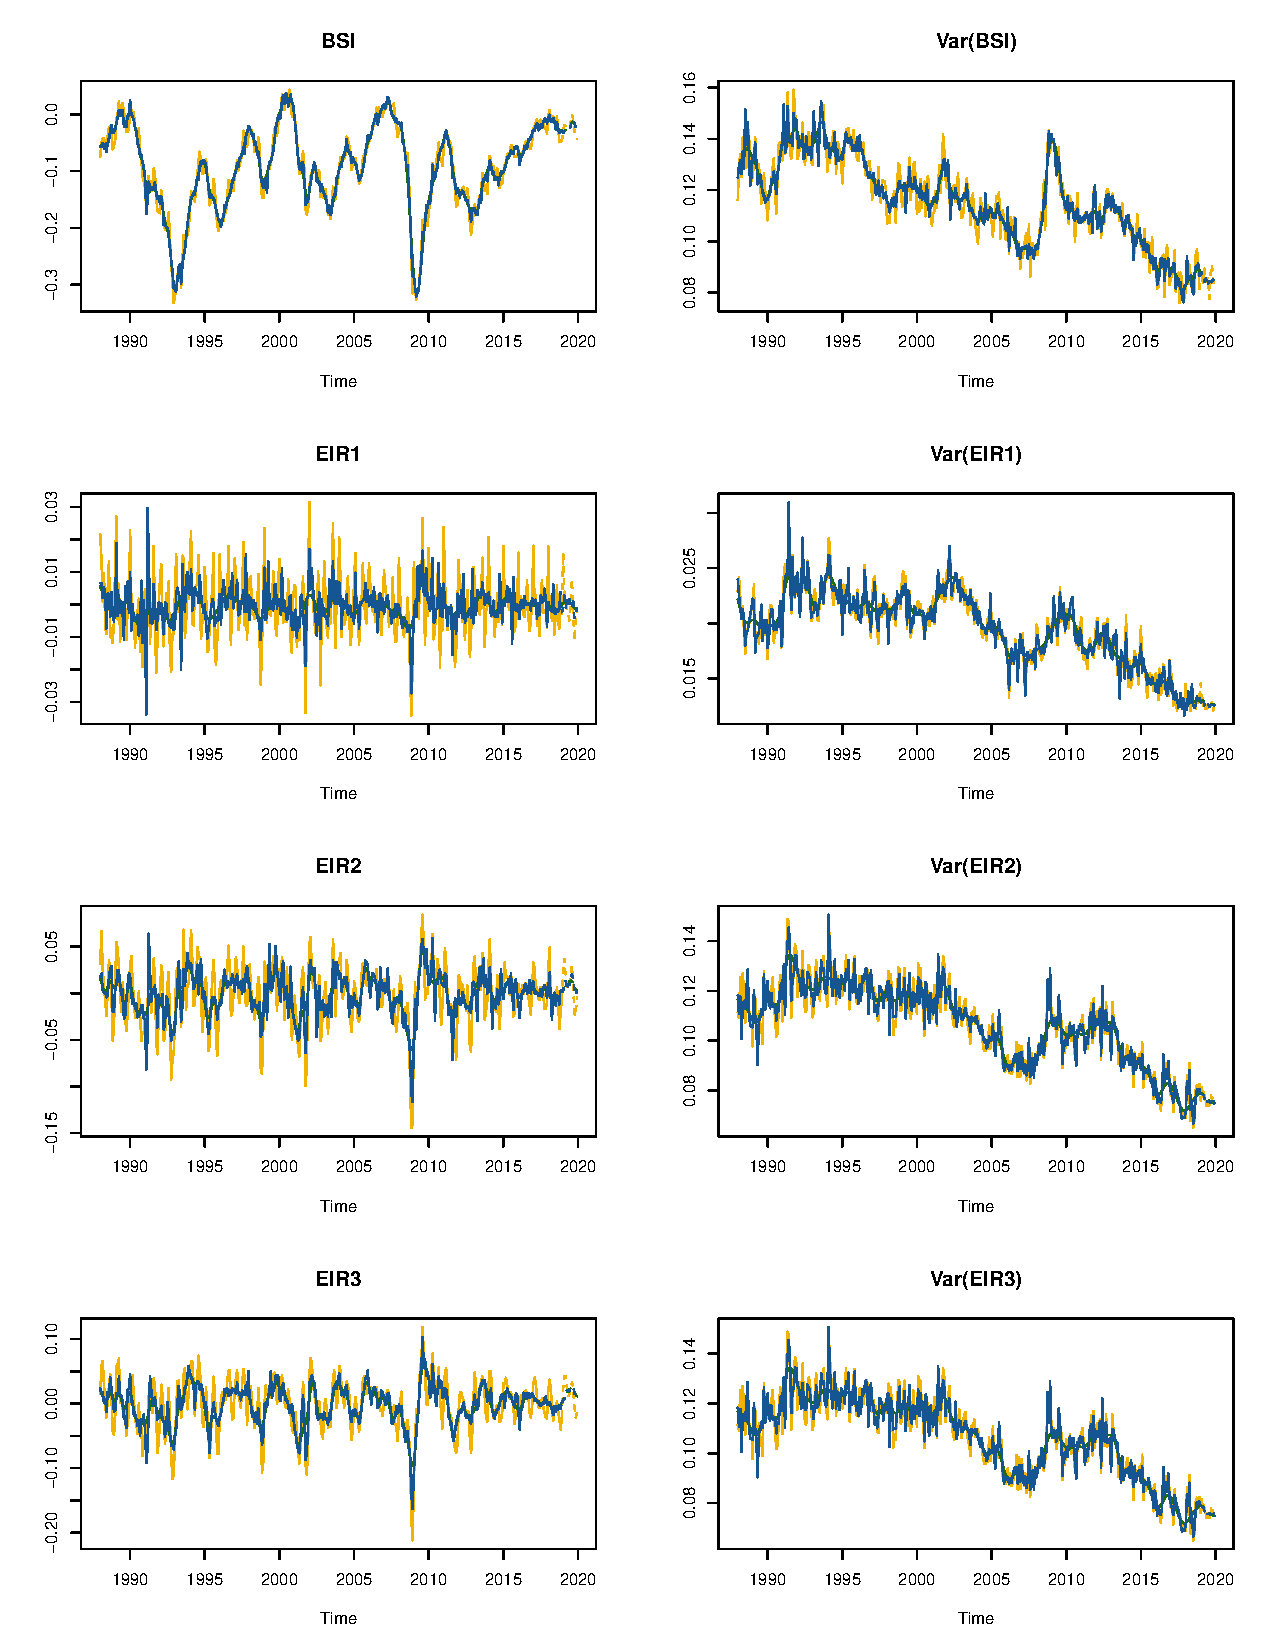
\includegraphics[scale=0.75]{Graphs/RJDemetra_plots.pdf}
    \caption{Plot of the industry business survey indicator (NS975), the indicator of the evolution of individual responses with the previous month (EIR1), two months (EIR2) and three months earlier (EIR3), with for each of them, their variance. The yellow lines are the raw data, the blue lines the seasonally corrected data and the green line is the trend of the variable.}
    \label{fig:seasonal ajusted rjdemetra}
\end{figure}


\section{Non-Response}

Non-response is a large domain of research when it comes to surveys. 
The theory converges to agree that there are three different ways non-response can be present. Responses can be missing completely at random, missing at random, or missing not at random.

Missing completely at random is usually hard to assume while missing not at random can be hard to account for.

% Considering the business survey, the non-response was explored, but since it's not the subject of the thesis, it will not be looked into more in dept.

The non-response of the business survey can be decomposed into two; non-participation to the survey and participants not responding to the survey.

Non-participation to the survey is difficult to study since not much trace is kept of the companies refusing to participate in the survey. As explained in the first chapter, the selection of participants uses stratification to account for the population at study. 
There is a bias that can come from the selection procedure since the survey is voluntary based, which means that if companies more prompt and motivated to participate are companies with a different profile compared to not motivated companies, there could be an issue.
The potential bias would be limited since the business survey is a panel survey and is interpreted as such.

Non-response of participants is another issue. 
The solution applied by the NBB in case of non-response is assuming that the respondent would have answered the same as the previous month, the method is called "Last Observation Carried Forward" (LOCF). 
It's widely used and can be understood in the case of the business survey, knowing that 

There is a large effort made by the NBB to contact respondents and send them reminders to make sure that non-response is as small as possible.
The response rate is usually around 95\%, which is quite high for a survey, therefore it can be assumed that non-response is not very important in the business survey.

% Before concluding it, since the mean study is the evolution rather than the indicator in itself, we plotted the non-response with the evolution of the year on year GDP to see if there seems to be a relation between the two. For example, we could expect more or less non-response during crises or in certain economic situations. Since the main interest of the BSI is to explain business cycles,




\section{Dropout and Attrition}

Dropout and Attrition are related to the structure and organisation of the survey. 
As explain in \autoref{sec:Recruitment of participants}, one's participants are recruited to participate in the business survey, they stay as long as they want. This brings two potential issues: companies who leave the survey create bias (dropout) and companies change of answering behaviour over time (attrition).

\subsection{Dropout}

The National Bank doesn't keep track from reasons why participants leave the survey. From discussions with the responsible persons for the survey at the NBB, the two mean reasons companies are leaving the survey are; (1) the company going bankrupt, acquired or merged and (2) the responsible person at the company leaves his job and the new contact person doesn't see the interest in participating in the survey.
This is an issue since it means that it's a certain type of companies that leave the survey. If this type of profile has a different opinion or respond differently than the remaining companies this will create bias. 


It could be argued that the bias is very diffused, due to the small number of companies leaving the survey each month. Again the fact that it's the evolution of the BSI that is important, means that we have a very small bias for each month (if we take a long period into account then the bias become larger) we are only comparing month to month evolution, and when the business survey is published, the 3-4 last year are showed.

It's not the subject of this work, so will not dive more into this bias, but we would recommend having a closer look into this for future researchers.

\subsection{Attrition}

Attrition, also called Panel Conditioning, is present when participants change there behaviour between different rounds of surveys. 
A very interesting master thesis was done about the Belgian labour force survey, where attrition was found to be significant \cite{priyana_hardjawidjaksana_investigating_2019}.
The Belgian labour force survey was convenient to test for attrition since the survey is answered by participants exactly four times with a lag of six months.
It was shown that indeed attrition was present in the survey.

In the case of the industry business survey, it's a harder to test for it since we have only two major periods of recruitment for the period at interest (1988 - 2018); in the early 1990 and between around 2000 with some companies been recruited. Other sectors have the same issue.


\begin{table}[htp!]  \centering \footnotesize 
  \caption{Correlation of time with different indicators } 
  \label{tab:corr attrition} 
\begin{tabular}{@{\extracolsep{5pt}} cccccc} 
\\[-1.8ex]\hline 
\hline \\[-1.8ex] 
 & GDP\_year & BSI & Var(BSI) & EIR & Var(EIR) \\ \hline \\[-1.8ex] 
Time & $-0.339$ & $0.133$ & $-0.807$ & $0.039$ & $-0.705$ \\ 
\hline \\[-1.8ex] 
\end{tabular} 
\end{table} 

An interesting approach to explore attrition and dropout is by looking at the correlations of the variances over time.
In \autoref{tab:corr attrition} it can be seen that there is a very large negative correlation between time and the variance of the BSI and the variance of the EIR. This can be interpreted as companies agreeing more and more over time and changing less and less there answers.
Without making any conclusions, the variance of BSI and the variance of EIR seems to show the present of dropout bias and/or attrition.

Same can be observed in Var(BSI) and Var(EIR) plots in \autoref{fig:seasonal ajusted rjdemetra} where, aside of the peak of variance during the economic crises of 2008, there is a general tendency of decreasing of the variance of the BSI and the different variances of EIR after the beginning of the century, the last time there was a large recruitment done.

The variance shows here an interest, it can be used to better understand the survey and the behaviour of respondents.
When looking at only the evolution of the business survey indicator, it's not possible to measure the vivacity of the survey.

It would be interesting to dive more into these issues, but this will be left for further research. 
In the context of this paper, it's important to notice the potential importance of attrition and dropout in the industry business survey and the importance of the variances to account for it.



\chapter{Exploratory Analysis}

The previous chapter already did some of the exploratory analysis.
Further observations of the different variables at hand will be done is a short descriptive statistics section.
In a second part, correlations among the variables will be looked at, and the last part will test autocorrelation.


\section{Descriptive Statistics}

The variables at hand are for the industry business survey and takes into account the four questions available on \autopageref{Appendix: Question NS975 description}, as explained in \autoref{sec:Questionnaire}.
The different variables are unweighted since the weights of the different respondents are only available for the surveys after 2008.

The data is seasonally corrected (see \autoref{sec:seasonal correction}) and is obtained for a 30 years period, from 1988 to 2018.
The year on year GDP calculation was explained in \autoref{eq:YoY GDP} and is here calculated for the Belgian economy.

The different variables at hand are summarised in \autoref{tab:descriptive statistics}. The YoY GDP has only one third as much observations as the other variables since it's a quarterly measure, while the survey is monthly. 
The table shows the scale of the different variables, for example, the industry BSI, over 30 years, never goes higher than 0.037 and never lower than -0.321.

The different variables are plotted in \autoref{plot:variables}, where it can be seen that the business survey indicator follow quite well the evolution of YoY GDP. 
The other variables, seem to react to major changes in the economy but are more volatile. 


\begin{table}[!htbp]  \centering \footnotesize 
  \caption{Descriptive Statistics} 
  \label{tab:descriptive statistics} 
\begin{tabular}{@{\extracolsep{5pt}}lccccccc} 
\\[-1.8ex]\hline 
\hline \\[-1.8ex] 
Statistic & \multicolumn{1}{c}{N} & \multicolumn{1}{c}{Mean} & \multicolumn{1}{c}{St. Dev.} & \multicolumn{1}{c}{Min} & \multicolumn{1}{c}{Pctl(25)} & \multicolumn{1}{c}{Pctl(75)} & \multicolumn{1}{c}{Max} \\ 
\hline \\[-1.8ex] 
YoY GDP     & 124       & 1.936 & 1.634 & $-$3.809 & 1.218 & 3.000 & 5.119 \\ 
BSI         & 372       & $-$0.094 & 0.075 & $-$0.321 & $-$0.141 & $-$0.033 & 0.037 \\ 
Var(BSI)    & 372       & 0.116 & 0.017 & 0.076 & 0.107 & 0.129 & 0.154 \\ 
EIR1        & 372       & $-$0.0003 & 0.006 & $-$0.034 & $-$0.004 & 0.003 & 0.030 \\ 
Var(EIR1)   & 372       & 0.020 & 0.003 & 0.012 & 0.017 & 0.022 & 0.031 \\ 
EIR2        & 372       & $-$0.001  & 0.024 & $-$0.116 & $-$0.013 & 0.013 & 0.064 \\ 
Var(EIR2)   & 372       & 0.107 & 0.016 & 0.067 & 0.095 & 0.119 & 0.151 \\ 
EIR3        & 372  & $-$0.002  & 0.031 & $-$0.163 & $-$0.018 & 0.018 & 0.103 \\ 
Var(EIR3)   & 372       & 0.123 & 0.019 & 0.075 & 0.109 & 0.137 & 0.166 \\ 
\hline \\[-1.8ex] 
\end{tabular} 
\end{table} 

\begin{figure}[!htbp]
    \centering
    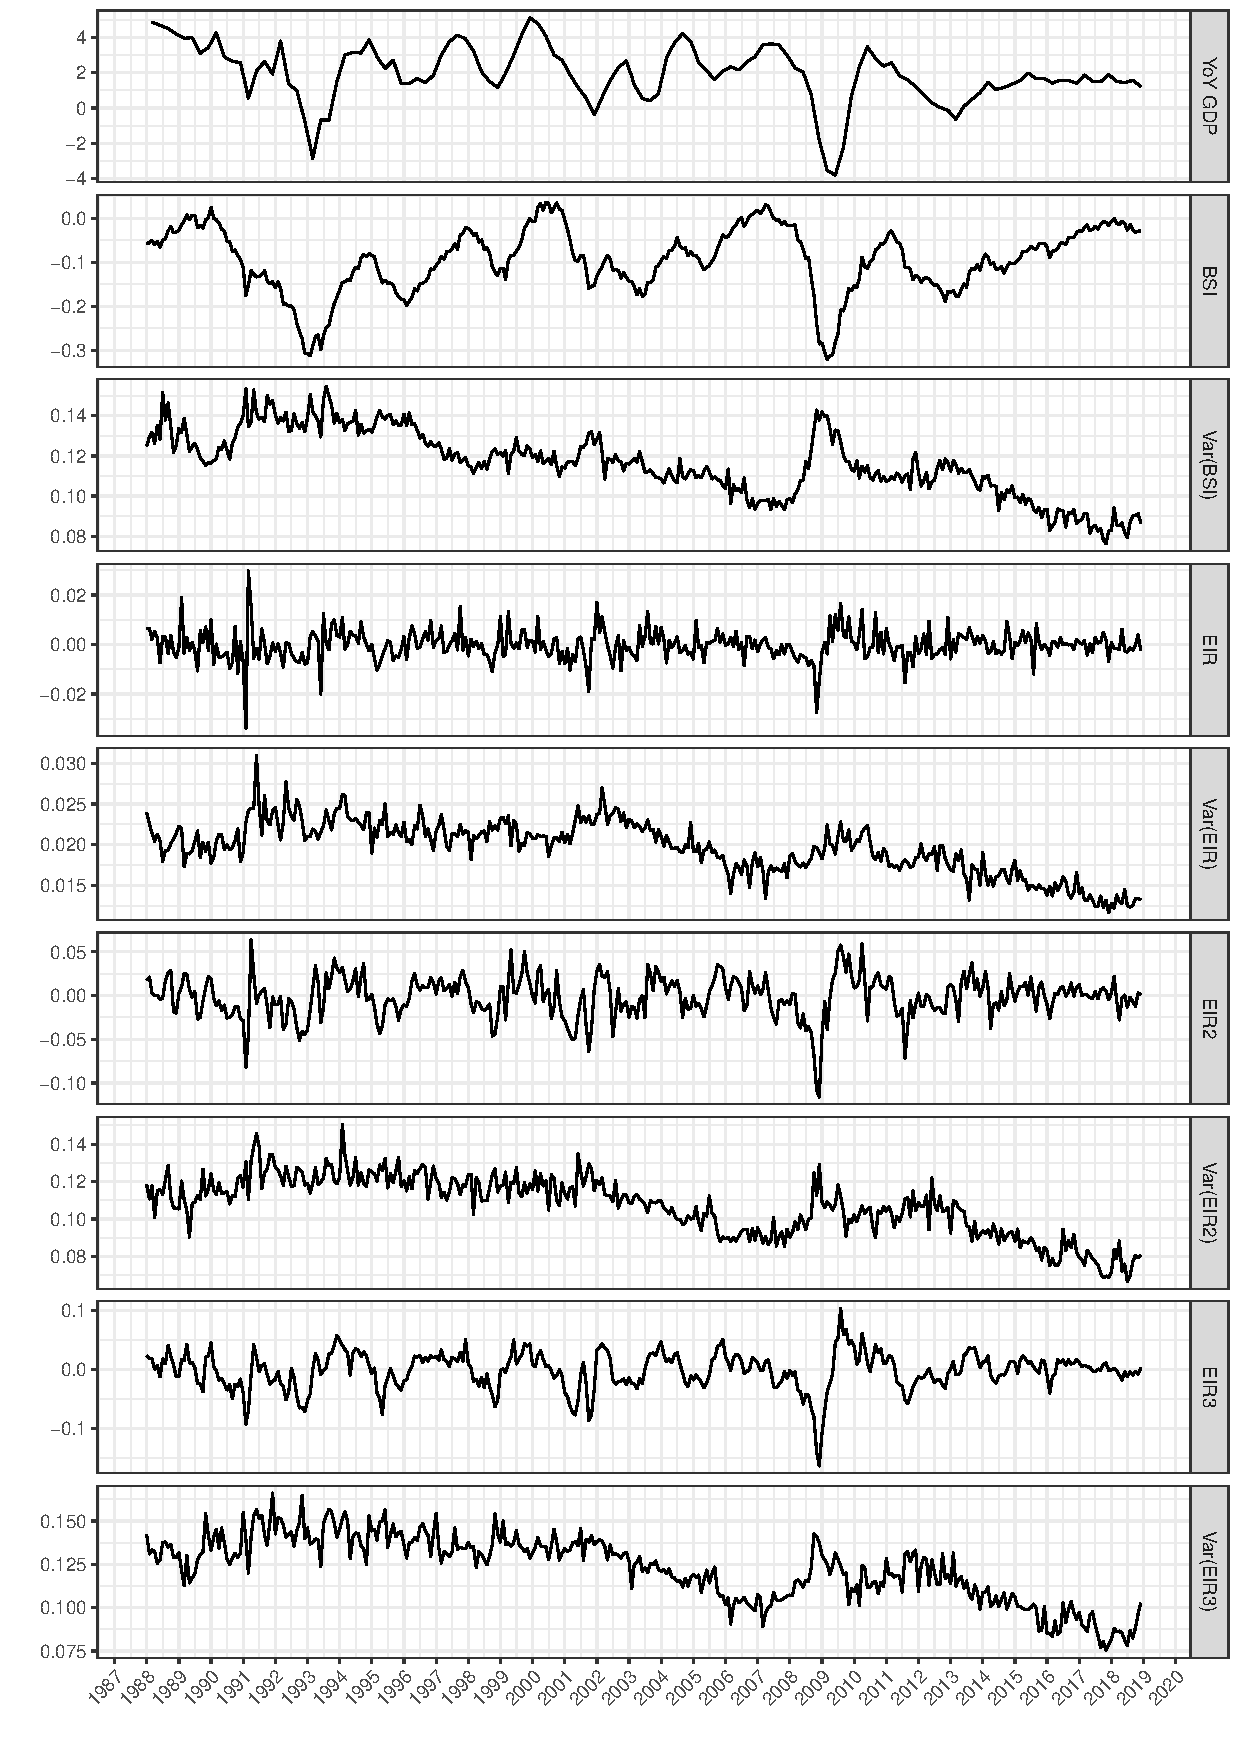
\includegraphics[scale=0.75]{Graphs/variables.pdf}
    \caption{Plot of the time series of YoY GDP, the BSI, the variance of the BSI and different EIR's (taking 1, 2 or 3 months differences) and their variance
    for the period 1988 to 2018}
    \label{plot:variables}
\end{figure}



\section{Correlation Analysis}

Belgian industry claims 25\% of the labour force in Belgium and was shown as a good indicator of the year to year GDP
\cite{de_greef_national_2009}.

\begin{figure}[H]
    \centering
    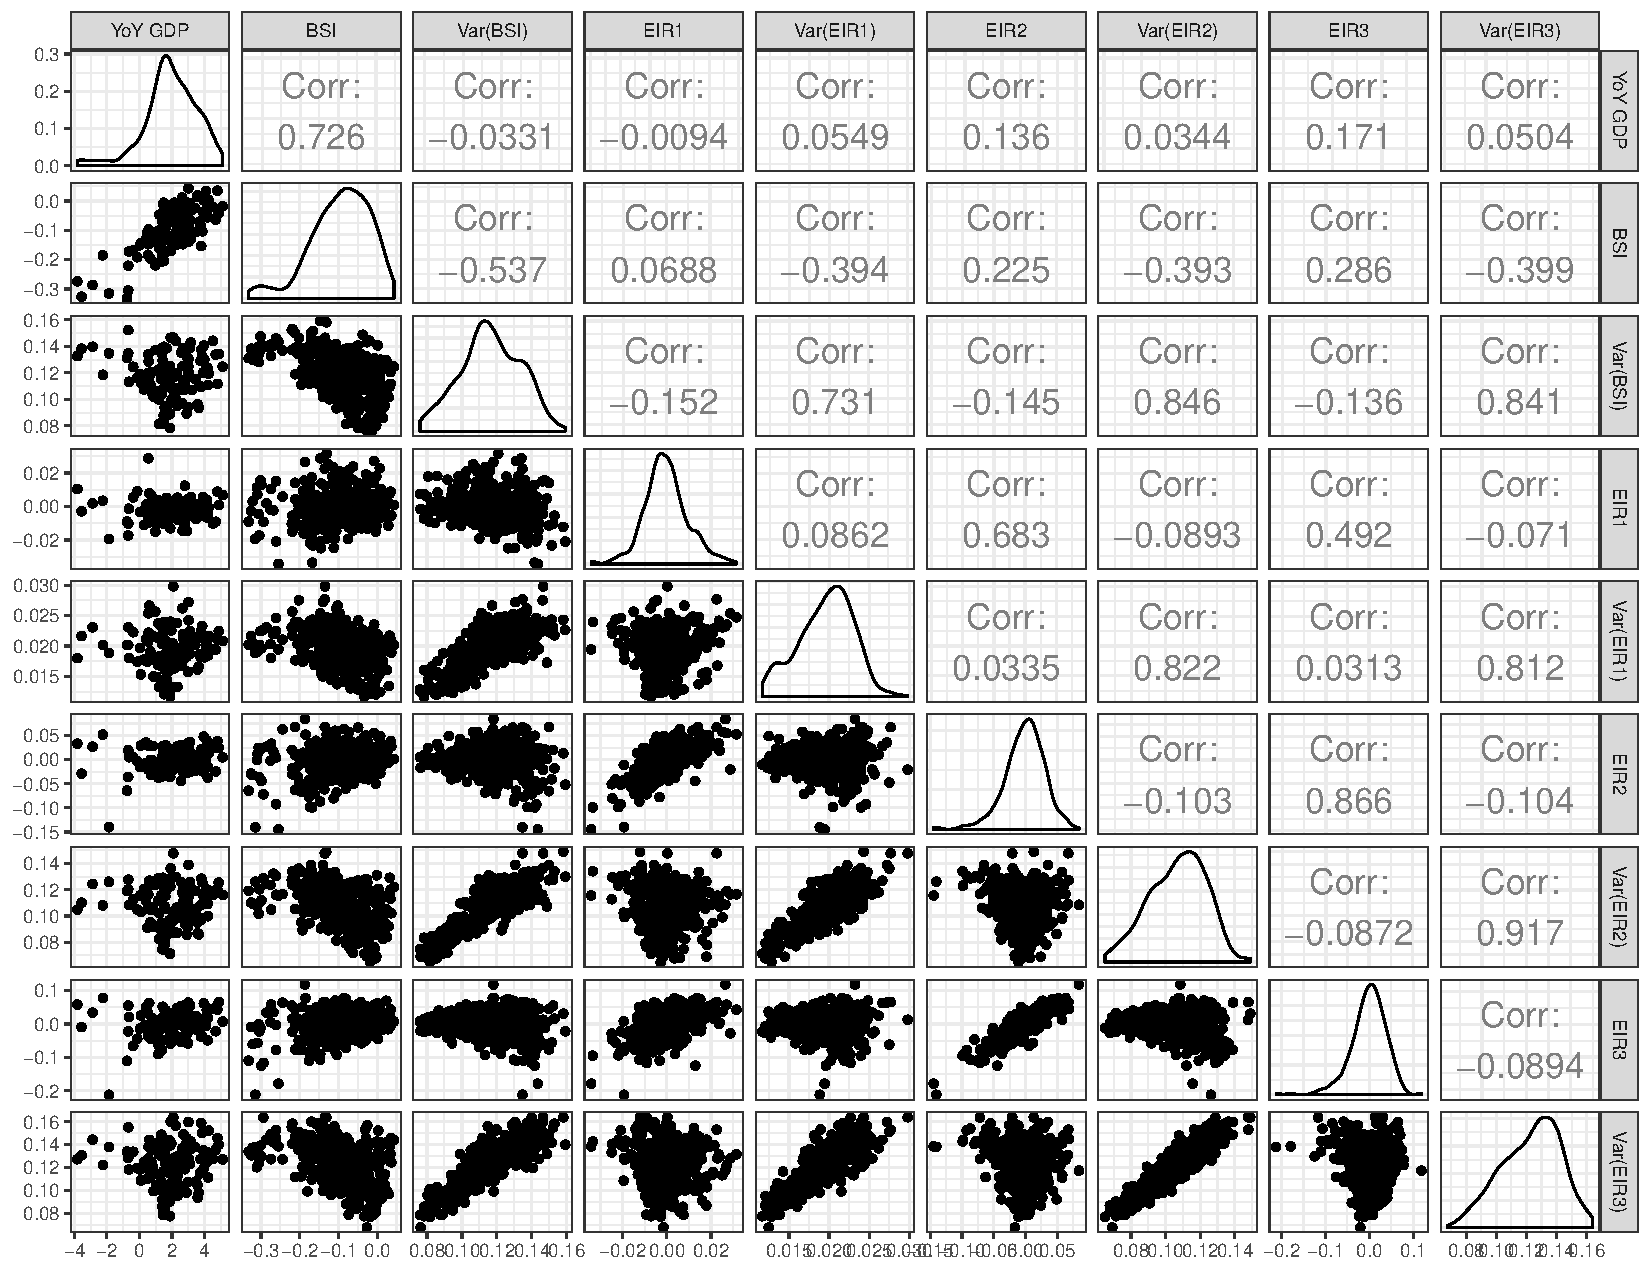
\includegraphics[scale=0.5]{Graphs/corr_indicators.pdf}
    \caption{Correlation plot of the YoY GDP, the business survey indicator and its variance, and the evolution of individual responses for 1,2 and three months lag and its according variances}
    \label{fig:corr indicators}
\end{figure}

\autoref{fig:corr indicators} shows the correlation matrix and plots of the different variables at hand. 
Several observations can be done.
First, it can be seen that the correlation between the business survey indicator and YoY GDP is very high while other variables have a rather small correlation with YoY GDP.

The correlation between the BSI and its variance is also high, this can be explained to some extend by the different observations done in \autoref{sec:properties variance}.
The same can not be said about the correlation between the EIR and its variance, since their correlation is small for the three different measures of EIR.

As could be forseen, the correlations between EIR1, EIR2 and EIR3 and the correlations between Var(EIR1), Var(EIR2) and Var(EIR3) are high.

The correlation between the different types of variances is also high, which can mean that they contain quite similar information.
With this definition it's interesting to look at the correlation between the BSI and the EIR since it's almost equal to zero. This can be interpreted as the two variables containing different information, if this will help to model Belgian growth will be discussed in the next chapter.


\section{Autocorrelation}

Autocorrelation, also known as serial correlation, is the correlation between an observation at time t and previous observations.

The method used here is to estimate the autocorrelation function and plot it, as can be seen in \autoref{fig:ACF}, where the correlation of a variables with its previous lags is shown. In the case of the YoY GDP, one lag means three months since the variables is quarterly, while for the other variables the lag corresponds to one month.
Several variables have high autocorrelation. The variances are highly correlated over time, as is the BSI. 
On the other hand, YoY GDP is slightly correlated with its three previous quarter values. 
For EIR1, the observations are not correlated at all with their previous observations. It can be observed that the autocorrelation increases by the amount of months taking into account for the EIR.


\begin{figure}[!htbp]
    \centering
    \captionsetup{justification=centering}
    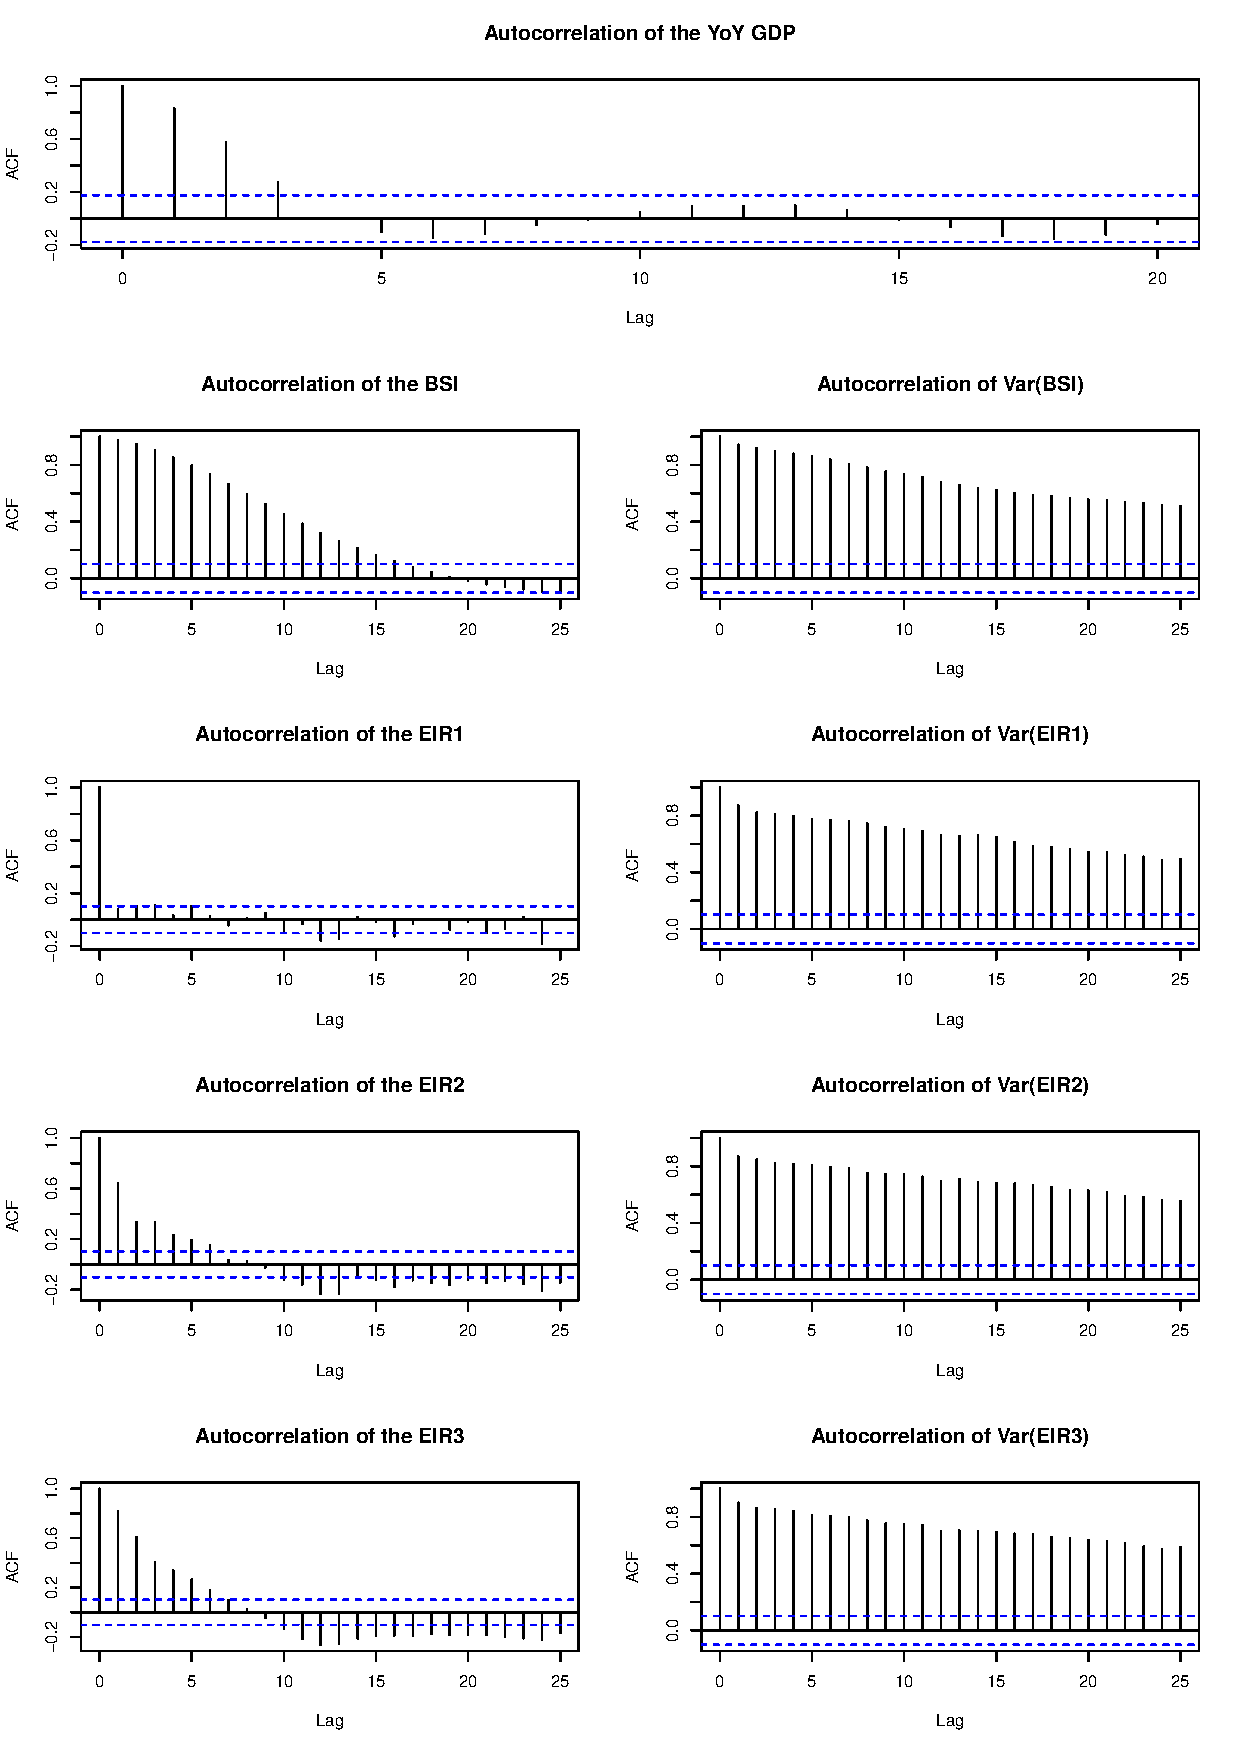
\includegraphics[scale=0.75]{Graphs/ACF.pdf}
    \caption{Autocorrelation plots for YoY GDP, the BSI, Var(BSI), EIR1, Var(EIR1), EIR2, Var(EIR2), EIR3 and Var(EIR3)}
    \label{fig:ACF}
\end{figure}


\section{Stationarity}

Test stationarity of the time series (ADF)
To test the stationarity of the time series, let’s run the Augmented Dickey-Fuller Test using the adf.test() function from the tseries R package.

First set the hypothesis test:

The null hypothesis H0 : that the time series is non-stationary The alternative hypothesis HA : that the time series is stationary

\begin{table}[!htbp] 
   \centering \footnotesize 
  \caption{ADF Test} 
  \label{tab:ADF Test} 
\begin{tabular}{@{\extracolsep{5pt}} ccccccccc} 
\\[-1.8ex]\hline 
\hline \\[-1.8ex] 
 & BSI & Var(BSI) & EIR1 & Var(EIR1) & EIR2 & Var(EIR2) & EIR3 & Var(EIR3)  \\ \hline \\[-1.8ex] 
p-value  & $< 0.01$ & 0.06 & $< 0.01$ & 0.26 & $< 0.01$ & 0.21 & $< 0.01$ & 0.12 \\
\hline \\[-1.8ex] 
\end{tabular} 
\end{table} 






\chapter{Linear Models}

The interest of this chapter is to use a model to test the pertinence of the variables in the short term prediction of the evolution of GDP.

As mention in \autoref{sec:nowcasting}, were nowcasting was discussed, there exist a large variety of different predictive models used in econometrics to predict the National Growth based on some explanatory variables.

The National Bank of Belgium for example, developed a State-Space model available in JDemetra+ \cite{de_antonio_liedo_nowcasting_2014}. Other well-known methods are ARIMA models, MIDAS and much more.

The interest of this paper is to explore the utility of the variance of the business survey indicator, the evolution of individual responses and its variance. 
To achieve this objective, it's important to use a model that account easily for the interest of each variable. Therefore, the linear model is applied here.

\section{Method}

The quarterly year on year GDP are set in the last month of the quarter. This is the common way to go to take a reasonable approach and still have some predictive properties.
Indeed of we look at \autoref{fig:time of the data}, it means that with the linear model it's possible to estimate quarterly YoY GDP one month before it's published. 
This means that the model will be estimated only with the indicators of the last month of each quarter. One the model is estimated, it's then possible to make predictions or estimations of YoY GDP for each month.


\begin{figure}[H]
     \centering \footnotesize
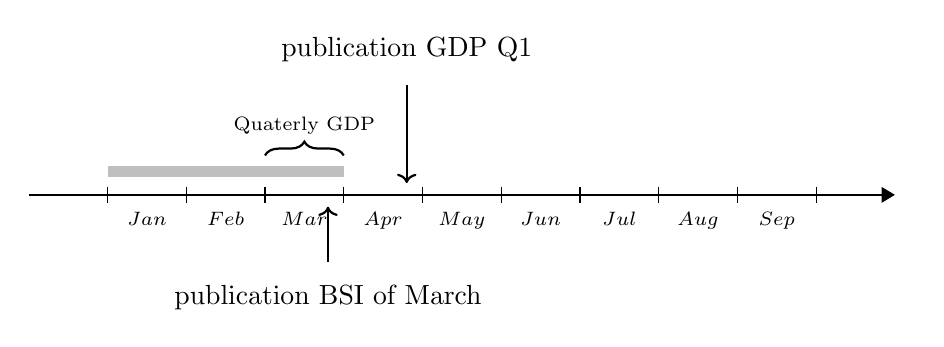
\begin{tikzpicture}
% draw horizontal line   
\draw[thick, -Triangle] (0,0) -- (\ImageWidth,0) node[font=\scriptsize,below left=3pt and -8pt]{ };
% draw vertical lines
\foreach \x in {1,...,10}
\draw (\x cm,3pt) -- (\x cm,-3pt);
\foreach \x/\descr in {1.5/Jan, 2.5/Feb, 3.5/Mar, 4.5/Apr, 5.5/May, 6.5/Jun, 7.5/Jul, 8.5/Aug,9.5/Sep}
\node[font=\scriptsize, text height=1.75ex,
text depth=.5ex] at (\x,-.3) {$\descr$};
% colored bar up
\foreach \x/\perccol in
{1/100,2/75,3/25}
\draw[lightgray, line width=4pt] 
(\x,.3) -- +(1,0);

% braces
\draw [thick ,decorate,decoration={brace,amplitude=5pt}] (3,0.5)  -- +(1,0) 
       node [black,midway,above=4pt, font=\scriptsize] {Quaterly GDP};
% time of publication
\node[align=center] at (4.8,1.85) {publication GDP Q1};
\draw [thick,->] (4.8,1.4) -- (4.8,0.15);
\node[align=center] at (3.8,-1.3) {publication BSI of March};
\draw [thick,->] (3.8,-0.85) -- (3.8,-0.15);
\end{tikzpicture}
    \caption{Timing of the observations}
    \label{fig:time of the data}
\end{figure}


\section{Linear Model}

The linear regression can be written as follow

\begin{eqnarray}
    \text{YoY GDP}_{t} = \beta_0 + \sum^n_{i = 1}
       \beta_{i} X_{t} + \epsilon_t 
\end{eqnarray}

Where $\beta_{0}$ is a constant, $\beta_{i}$  are the different regression coefficients of the monthly predictors ( $X_{t}$) and $\epsilon_t$ is the error term.

The first approach here is to propose five different models (\autoref{eq:model1}-\ref{eq:model5}) and compare them.
The simple model takes as unique regressor the business survey indicator

\begin{eqnarray}
    \text{YoY GDP}_{t} = \beta_0 + \beta_{1} \BSI_{t} + \epsilon_t \label{eq:model1} 
\end{eqnarray}

The other model takes the business survey indicator and its variance as regressors

\begin{eqnarray}
    \text{YoY GDP}_{t} = \beta_0 + \beta_{1} \BSI_{t}  + \beta_{2} \Var(\BSI)_{t} + \epsilon_t \label{eq:model2}
\end{eqnarray}

And three different models where the three evolution of individual responses with their variances are each time added to the models including the business survey and its variance

\begin{eqnarray}
    \text{YoY GDP}_{t} = \beta_0 + \beta_{1} \BSI_{t}  + \beta_{2} \Var(\BSI)_{t} + \beta_{3} \EIR1_{t}  + \beta_{4} \Var(\EIR1)_{t} + \epsilon_t \label{eq:model3}
\end{eqnarray}
\begin{eqnarray}
    \text{YoY GDP}_{t} = \beta_0 + \beta_{1} \BSI_{t}  + \beta_{2} \Var(\BSI)_{t} + \beta_{5} \EIR2_{t}  + \beta_{6} \Var(\EIR2)_{t} + \epsilon_t \label{eq:model4}
\end{eqnarray}
\begin{eqnarray}
    \text{YoY GDP}_{t} = \beta_0 + \beta_{1} \BSI_{t}  + \beta_{2} \Var(\BSI)_{t} + \beta_{7} \EIR3_{t}  + \beta_{8} \Var(\EIR3)_{t} + \epsilon_t  \label{eq:model5}
\end{eqnarray}


\begin{table}[H] \centering \footnotesize
  \caption{Linear regressions} 
  \label{tab:models comparaison 1} 
\begin{tabular}{@{\extracolsep{5pt}}lD{.}{.}{-3} D{.}{.}{-3} D{.}{.}{-3} D{.}{.}{-3} D{.}{.}{-3} } 
\\[-1.8ex]\hline 
\hline \\[-1.8ex] 
 & \multicolumn{5}{c}{Linear Regression} \\ 
\cline{2-6} 
\\[-1.8ex] & \multicolumn{5}{c}{year on year GDP (in \%)} \\ 
\\[-1.8ex] & \multicolumn{1}{c}{(\ref{eq:model1})} & \multicolumn{1}{c}{(\ref{eq:model2})} & \multicolumn{1}{c}{(\ref{eq:model3})} & \multicolumn{1}{c}{(\ref{eq:model4})} & \multicolumn{1}{c}{(\ref{eq:model5})}\\ 
\hline \\[-1.8ex] 
 Constant & 3.429^{***} & -1.740^{***} & -1.821^{***} & -1.756^{***} & -1.729^{***} \\ 
  & (0.160) & (0.631) & (0.615) & (0.635) & (0.633) \\ 
  & & & & & \\ 
 BSI & 15.773^{***} & 21.443^{***} & 21.548^{***} & 21.310^{***} & 21.044^{***} \\ 
  & (1.317) & (1.252) & (1.224) & (1.306) & (1.313) \\ 
  & & & & & \\ 
 Var(BSI) &  & 49.102^{***} & 36.477^{***} & 40.631^{***} & 38.777^{***} \\ 
  &  & (5.869) & (8.089) & (11.895) & (11.081) \\ 
  & & & & & \\ 
 EIR1 &  &  & -28.718^{**} &  &  \\ 
  &  &  & (13.792) &  &  \\ 
  & & & & & \\ 
 Var(EIR1) &  &  & 78.555^{**} &  &  \\ 
  &  &  & (35.187) &  &  \\ 
  & & & & & \\ 
 EIR2 &  &  &  & -0.709 &  \\ 
  &  &  &  & (3.878) &  \\ 
  & & & & & \\ 
 Var(EIR2) &  &  &  & 9.213 &  \\ 
  &  &  &  & (11.207) &  \\ 
  & & & & & \\ 
 EIR3 &  &  &  &  & 1.290 \\ 
  &  &  &  &  & (2.610) \\ 
  & & & & & \\ 
 Var(EIR3) &  &  &  &  & 9.401 \\ 
  &  &  &  &  & (8.598) \\ 
  & & & & & \\ 
\hline \\[-1.8ex] 
Observations & \multicolumn{1}{c}{124} & \multicolumn{1}{c}{124} & \multicolumn{1}{c}{124} & \multicolumn{1}{c}{124} & \multicolumn{1}{c}{124} \\ 
R$^{2}$ & \multicolumn{1}{c}{0.540} & \multicolumn{1}{c}{0.709} & \multicolumn{1}{c}{0.728} & \multicolumn{1}{c}{0.711} & \multicolumn{1}{c}{0.712} \\ 
Adjusted R$^{2}$ & \multicolumn{1}{c}{0.537} & \multicolumn{1}{c}{0.704} & \multicolumn{1}{c}{0.719} & \multicolumn{1}{c}{0.701} & \multicolumn{1}{c}{0.702} \\ 
Resid. Std. Er. & \multicolumn{1}{c}{1.112} & \multicolumn{1}{c}{0.889} & \multicolumn{1}{c}{0.866} & \multicolumn{1}{c}{0.894} & \multicolumn{1}{c}{0.891} \\ 
AIC & \multicolumn{1}{c}{382.292} & \multicolumn{1}{c}{327.699} & \multicolumn{1}{c}{323.086} & \multicolumn{1}{c}{330.907} & \multicolumn{1}{c}{330.293} \\ 
BIC & \multicolumn{1}{c}{390.753} & \multicolumn{1}{c}{338.980} & \multicolumn{1}{c}{340.008} & \multicolumn{1}{c}{347.829} & \multicolumn{1}{c}{347.215} \\ 
\hline 
\hline \\[-1.8ex] 
\textit{Note:}  & \multicolumn{5}{r}{$^{*}$p$<$0.1; $^{**}$p$<$0.05; $^{***}$p$<$0.01} \\ 
\end{tabular} 
\end{table} 


The estimates can be seen in \autoref{tab:models comparaison 1} for the five regressions. Some goodness of fit measures are also available. 
Those first results show the limited interest of EIR2 and EIR3 since the model with EIR1 and its variance (\autoref{eq:model3}) is better performing according to all the results than the two other models (\autoref{eq:model4} and \autoref{eq:model5}).

The other observation that can be done is that the interest of the variance in the prediction seems significant since adding, next to the information of the business survey, increases the Adjusted R$^2$ by 0.151. The model is also better according to AIC and BIC results.

\begin{table}[!htbp]
    \centering \footnotesize
\begin{tabular}{@{\extracolsep{5pt}} cccccccc} 
\\[-1.8ex]\hline 
\hline \\[-1.8ex] 
                 & RMSE & MAE & MPE & MAPE & MASE \\ \hline
\autoref{eq:model1} & 1.103 &0.93 &-27.657 & 86.696 & 0.764 \\
\autoref{eq:model2} & 0.878 &0.697 & -10.923 & 61.185 & 0.573 \\
\autoref{eq:model3} & 0.848 &0.674 & -12.455 & 55.698 & 0.554 \\
\autoref{eq:model4} & 0.875 &0.699 & -12.757 & 62.707 & 0.574 \\
\autoref{eq:model5} & 0.873 &0.689 & -9.83 & 59.311 & 0.566 \\ \hline
    \end{tabular}
    \caption{Accuracy}
    \label{tab:accuracy measures}
\end{table}


RMSE: Root Mean Squared Error

MAE: Mean Absolute Error

MPE: Mean Percentage Error

MAPE: Mean Absolute Percentage Error

MASE: Mean Absolute Scaled Error

\subsection{Diebold-Mariano Test}

\cite{diebold_comparing_1995}

DM = 1.2727, Forecast horizon = 1, Loss function power = 2, p-value = 0.2055
alternative hypothesis: two.sided


\begin{table}[!htbp]
    \centering \footnotesize
    \begin{tabular}{c|c|c|c}
        p-values & \autoref{eq:model1} & \autoref{eq:model2} & \autoref{eq:model3} \\ \hline
        \autoref{eq:model1} &    & 0.00005126  & 0.00002586    \\
        \autoref{eq:model2} &    &        & 0.2055        \\
        \autoref{eq:model3} &    &        &      \\
    \end{tabular}
    \caption{Diebold-Mariano Tests}
    \label{tab:Diebold-Mariano}
\end{table}


\begin{figure}[!htbp]
    \centering
    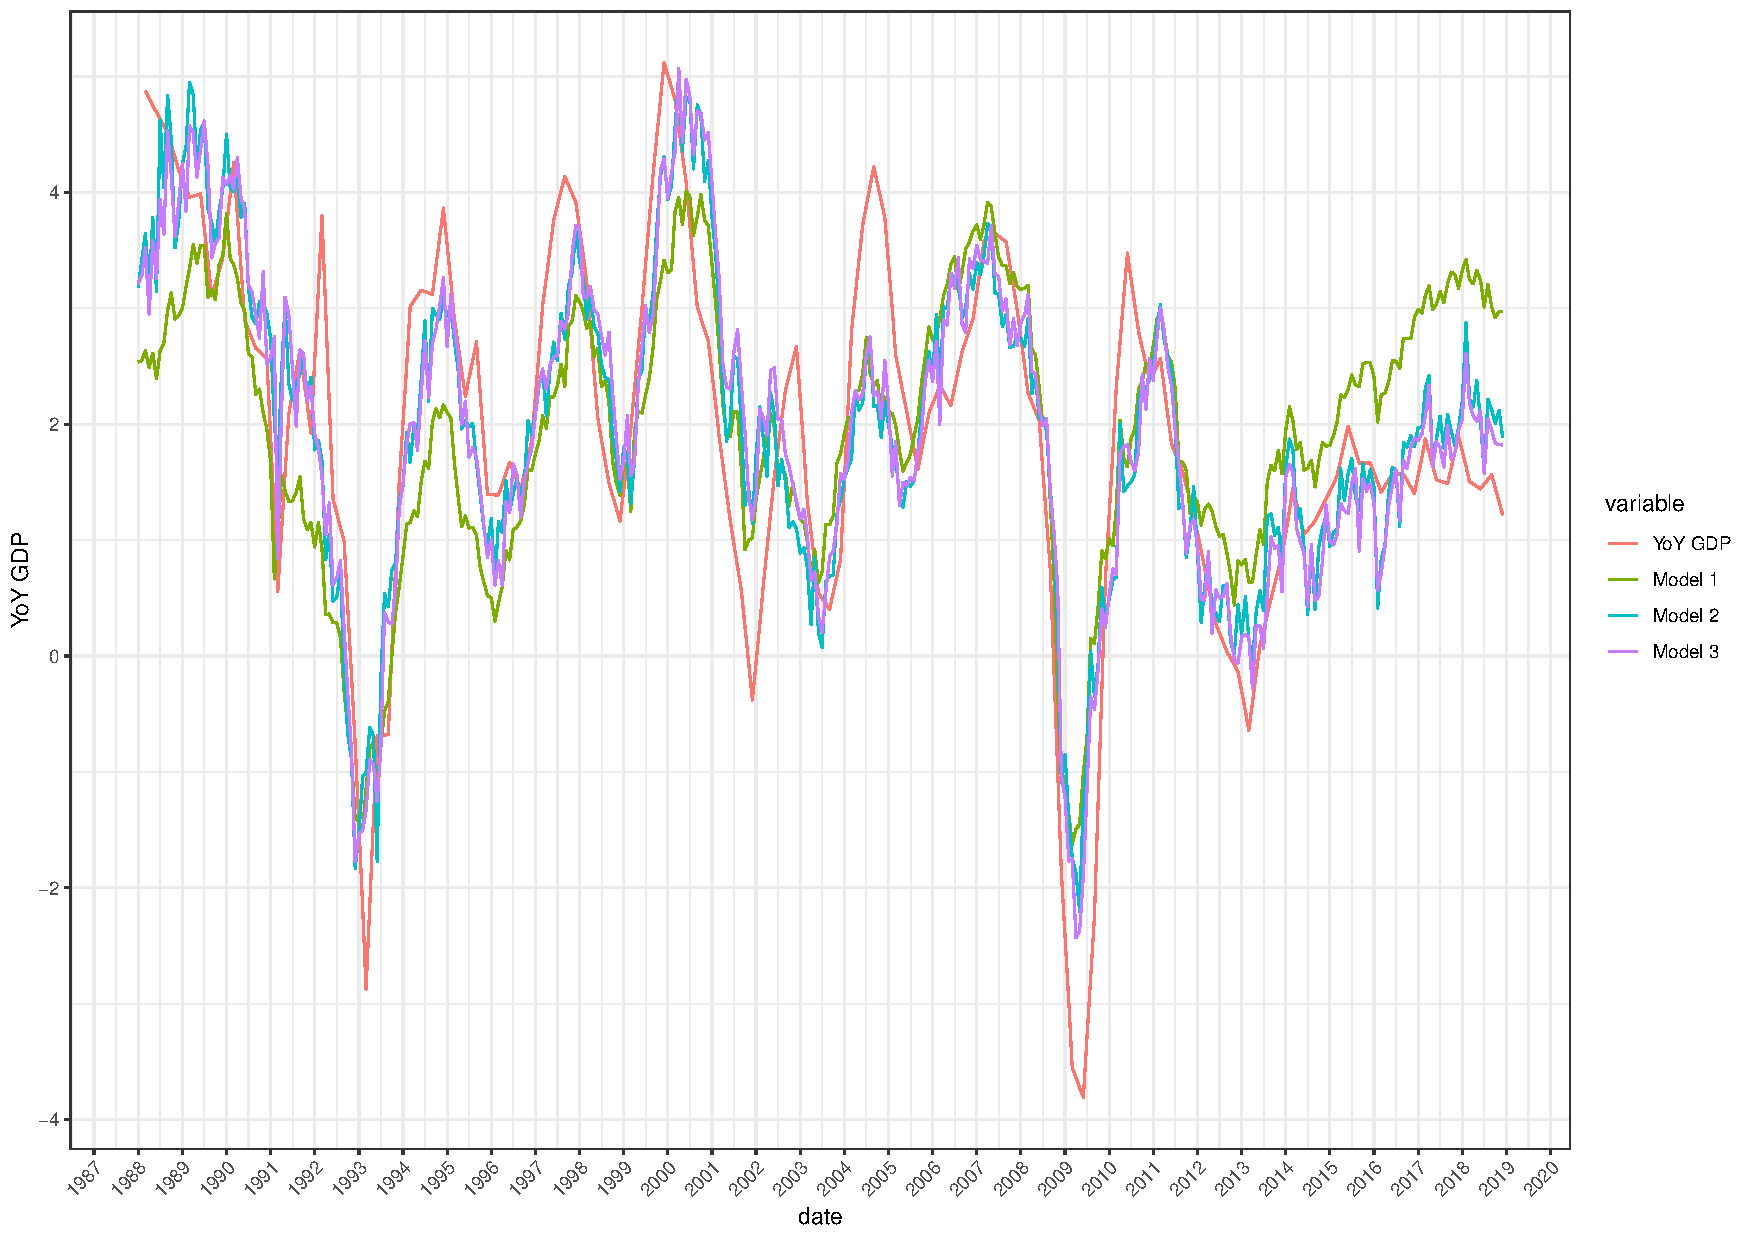
\includegraphics[scale=0.6]{Graphs/predictions1.pdf}
    \caption{Plot of year on year GDP and the different estimation from model 1, 2 and 3}
    \label{fig:predictions1}
\end{figure}



\section{Model Selection}

Since there are a large among of different possible models when having eight different regressors, some procedure needs to be chosen to look for the best model.

The method applied here is a step procedure where AIC is used to select the best model.
Three different selection algorithms will be applied; (1) forward, (2) backward and  (3) both. 
The three methods are all based on Akaike's information criterion (AIC) as measure of goodness of fit. They differ in the sense that the first (1) starts from a model with no regressors and adds one by one the regressors that improve the most the model fit, the second (2) does the opposite, it starts with the full model and takes out the variables that don't improve the model fit and the last (3) is a mixed of the two previous methods.

The results of the three different methods converge to the model already proposed in \autoref{eq:model3}, where BSI, Var(BSI), EIR1 and Var(EIR1) are the regressors.

From the different results, it can already be stated that EIR1 and its variance are bringing more in the modelling of the YoY GDP than EIR2 and EIR3 with their variances.

It was also seen that the variance of the BSI improves the model quite largely and that EIR1 and its variance can also add some information.


Following those results, there are two good candidates; \autoref{eq:model2} and \ref{eq:model3}. Those are the two models that we will be further looked into and compared to the simplest model only including the BSI.












\subsection{Out-of-Sample Performances}

\begin{table}[!htbp] \centering 
  \caption{} 
  \label{} 
\begin{tabular}{@{\extracolsep{5pt}}lD{.}{.}{-3} D{.}{.}{-3} D{.}{.}{-3} } 
\\[-1.8ex]\hline 
\hline \\[-1.8ex] 
 & \multicolumn{3}{c}{Linear Regression} \\ 
\cline{2-4} 
\\[-1.8ex] & \multicolumn{3}{c}{Year on Year GDP (in \%)} \\ 
\\[-1.8ex] & \multicolumn{1}{c}{(1)} & \multicolumn{1}{c}{(2)} & \multicolumn{1}{c}{(3)}\\ 
\hline \\[-1.8ex] 
 Constant & 4.437^{***} & 0.660 & -0.519 \\ 
  & (0.211) & (1.899) & (2.041) \\ 
  & & & \\ 
 BSI & 17.374^{***} & 19.212^{***} & 20.327^{***} \\ 
  & (1.547) & (1.758) & (1.813) \\ 
  & & & \\ 
 Var(BSI) &  & 30.545^{*} & 31.371^{**} \\ 
  &  & (15.269) & (14.992) \\ 
  & & & \\ 
 EIR1 &  &  & -37.120^{**} \\ 
  &  &  & (17.899) \\ 
  & & & \\ 
 Var(EIR1) &  &  & 53.535 \\ 
  &  &  & (52.433) \\ 
  & & & \\ 
\hline \\[-1.8ex] 
Observations & \multicolumn{1}{c}{48} & \multicolumn{1}{c}{48} & \multicolumn{1}{c}{48} \\ 
R$^{2}$ & \multicolumn{1}{c}{0.733} & \multicolumn{1}{c}{0.754} & \multicolumn{1}{c}{0.779} \\ 
Adjusted R$^{2}$ & \multicolumn{1}{c}{0.727} & \multicolumn{1}{c}{0.744} & \multicolumn{1}{c}{0.758} \\ 
Residual Std. Error & \multicolumn{1}{c}{0.851} & \multicolumn{1}{c}{0.825} & \multicolumn{1}{c}{0.801} \\ 
F Statistic & \multicolumn{1}{c}{126.060$^{***}$} & \multicolumn{1}{c}{69.144$^{***}$} & \multicolumn{1}{c}{37.845$^{***}$} \\ 
\hline 
\hline \\[-1.8ex] 
\textit{Note:}  & \multicolumn{3}{r}{$^{*}$p$<$0.1; $^{**}$p$<$0.05; $^{***}$p$<$0.01} \\ 
\end{tabular} 
\end{table} 


\begin{figure}[!htbp]
    \centering
    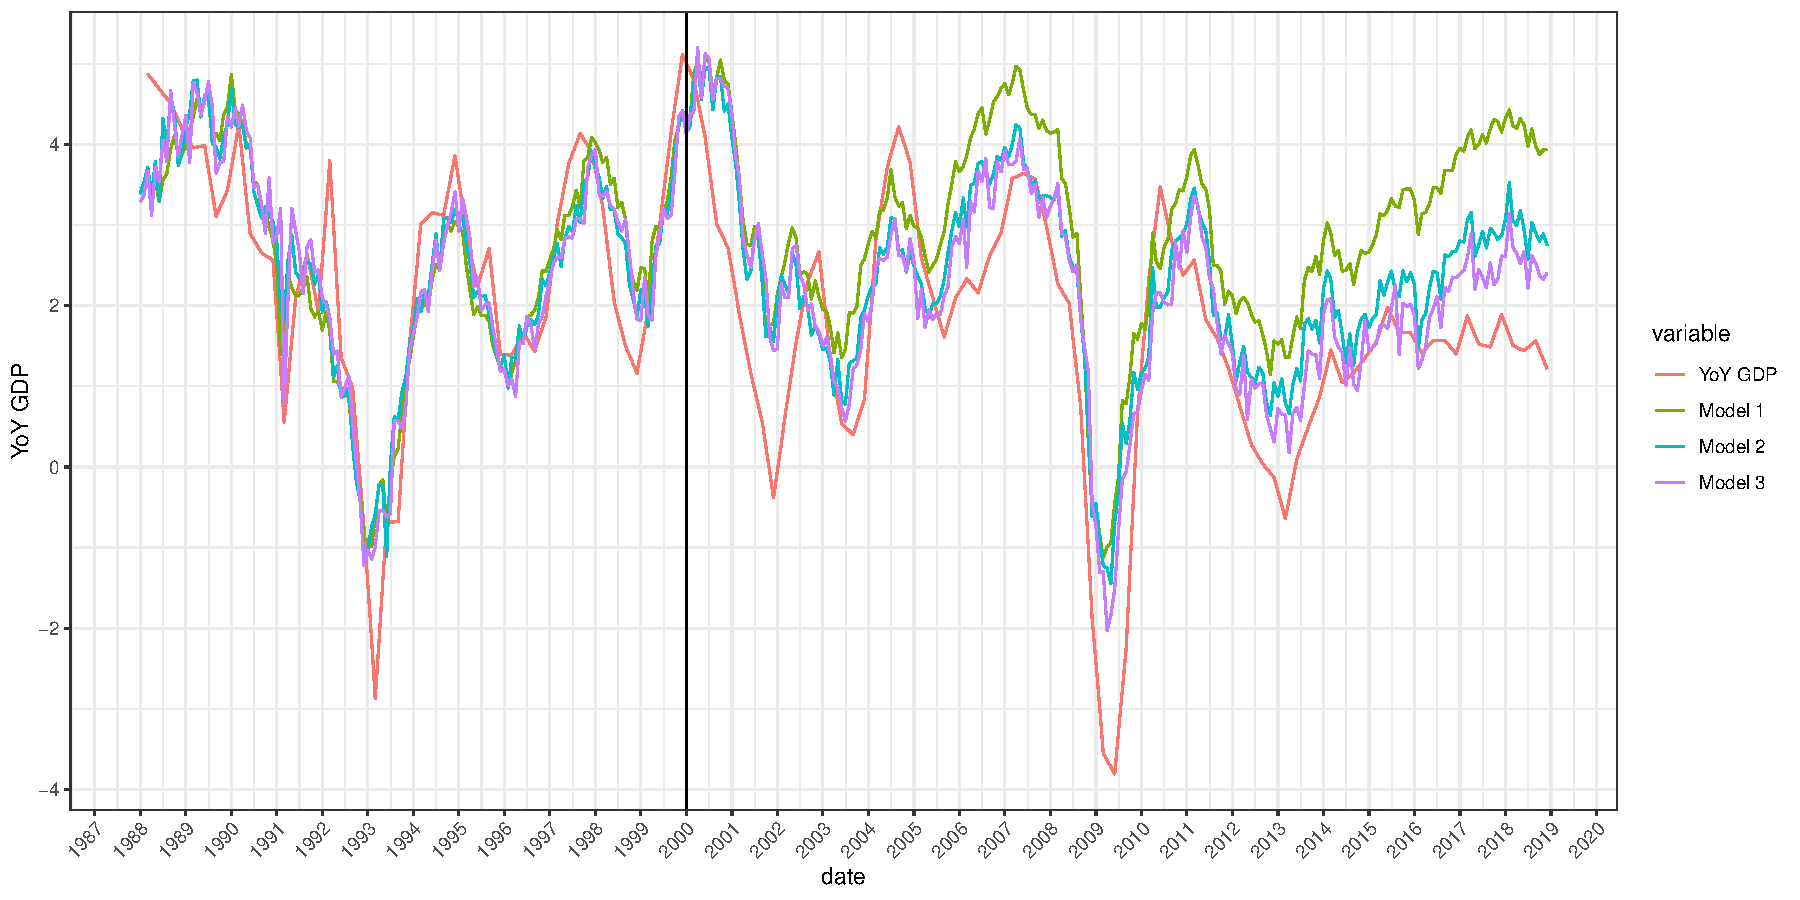
\includegraphics[scale=0.5]{Graphs/predictions2.pdf}
    \caption{Plot of year on year GDP and the different estimation from model 1, 2 and 3}
    \label{fig:predictions1}
\end{figure}


\begin{figure}[!htbp]
    \centering
    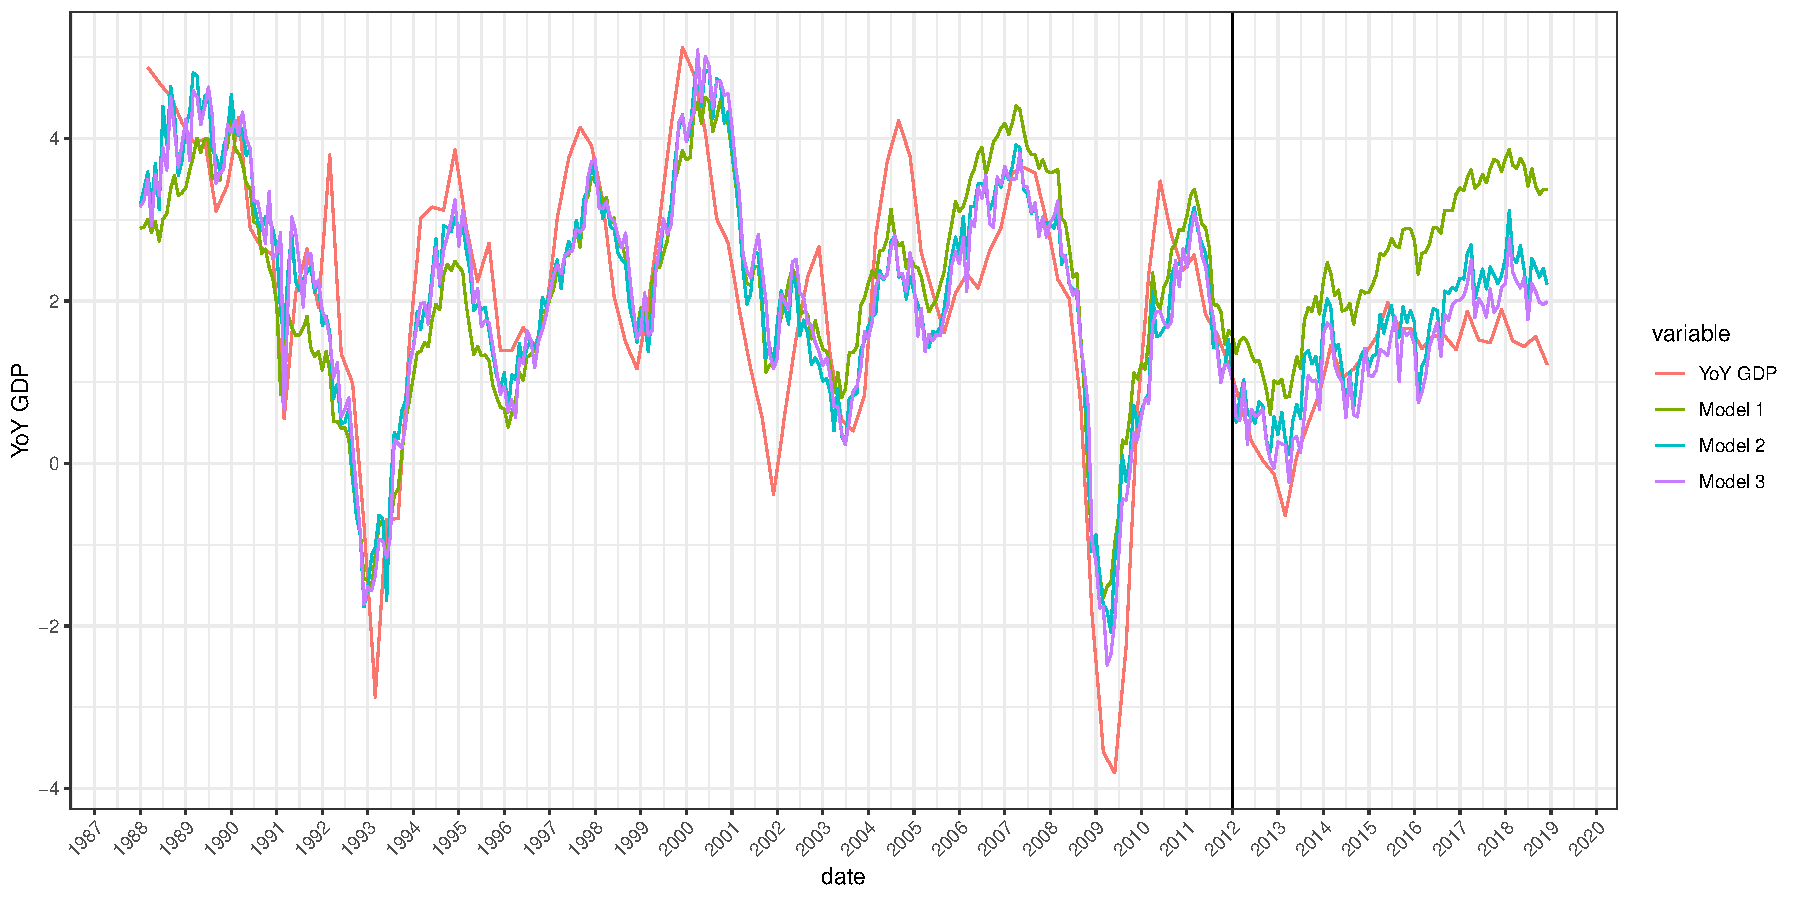
\includegraphics[scale=0.5]{Graphs/predictions3.pdf}
    \caption{Plot of year on year GDP and the different estimation from model 1, 2 and 3}
    \label{fig:predictions1}
\end{figure}




\begin{landscape}
    \section{Model with before 2000 data}

\begin{table}[!htbp]  \centering \footnotesize
  \caption{} 
  \label{} 
\begin{tabular}{@{\extracolsep{5pt}}lD{.}{.}{-3} D{.}{.}{-3} D{.}{.}{-3} D{.}{.}{-3} D{.}{.}{-3} D{.}{.}{-3} } 
\\[-1.8ex]\hline 
\hline \\[-1.8ex] 
 & \multicolumn{6}{c}{Linear Regression} \\ 
\cline{2-7} 
\\[-1.8ex] & \multicolumn{6}{c}{year on year GDP (in \%)} \\ 
\\[-1.8ex] & \multicolumn{1}{c}{(1)} & \multicolumn{1}{c}{(2)} & \multicolumn{1}{c}{(3)} & \multicolumn{1}{c}{(4)} & \multicolumn{1}{c}{(5)} & \multicolumn{1}{c}{(6)}\\ 
\hline \\[-1.8ex] 
 Constant & 3.429^{***} & -1.740^{***} & -1.821^{***} & 4.437^{***} & 0.660 & -0.519 \\ 
  & (0.160) & (0.631) & (0.615) & (0.211) & (1.899) & (2.041) \\ 
  & & & & & & \\ 
 BSI & 15.773^{***} & 21.443^{***} & 21.548^{***} & 17.374^{***} & 19.212^{***} & 20.327^{***} \\ 
  & (1.317) & (1.252) & (1.224) & (1.547) & (1.758) & (1.813) \\ 
  & & & & & & \\ 
 Var(BSI) &  & 49.102^{***} & 36.477^{***} &  & 30.545^{*} & 31.371^{**} \\ 
  &  & (5.869) & (8.089) &  & (15.269) & (14.992) \\ 
  & & & & & & \\ 
 EIR1 &  &  & -28.718^{**} &  &  & -37.120^{**} \\ 
  &  &  & (13.792) &  &  & (17.899) \\ 
  & & & & & & \\ 
 Var(EIR1) &  &  & 78.555^{**} &  &  & 53.535 \\ 
  &  &  & (35.187) &  &  & (52.433) \\ 
  & & & & & & \\ 
\hline \\[-1.8ex] 
Observations & \multicolumn{1}{c}{124} & \multicolumn{1}{c}{124} & \multicolumn{1}{c}{124} & \multicolumn{1}{c}{48} & \multicolumn{1}{c}{48} & \multicolumn{1}{c}{48} \\ 
R$^{2}$ & \multicolumn{1}{c}{0.540} & \multicolumn{1}{c}{0.709} & \multicolumn{1}{c}{0.728} & \multicolumn{1}{c}{0.733} & \multicolumn{1}{c}{0.754} & \multicolumn{1}{c}{0.779} \\ 
Adjusted R$^{2}$ & \multicolumn{1}{c}{0.537} & \multicolumn{1}{c}{0.704} & \multicolumn{1}{c}{0.719} & \multicolumn{1}{c}{0.727} & \multicolumn{1}{c}{0.744} & \multicolumn{1}{c}{0.758} \\ 
Res. Std. Error & \multicolumn{1}{c}{1.112} & \multicolumn{1}{c}{0.889} & \multicolumn{1}{c}{0.866} & \multicolumn{1}{c}{0.851} & \multicolumn{1}{c}{0.825} & \multicolumn{1}{c}{0.801} \\ 
F Statistic & \multicolumn{1}{c}{143.463$^{***}$} & \multicolumn{1}{c}{147.283$^{***}$} & \multicolumn{1}{c}{79.773$^{***}$} & \multicolumn{1}{c}{126.060$^{***}$} & \multicolumn{1}{c}{69.144$^{***}$} & \multicolumn{1}{c}{37.845$^{***}$} \\ 
\hline 
\hline \\[-1.8ex] 
\textit{Note:}  & \multicolumn{6}{r}{$^{*}$p$<$0.1; $^{**}$p$<$0.05; $^{***}$p$<$0.01} \\ 
\end{tabular} 
\end{table} 

\end{landscape}

\begin{landscape}
    \begin{table}[!htbp]  \centering \footnotesize 
  \caption{} 
  \label{} 
\begin{tabular}{@{\extracolsep{5pt}}lD{.}{.}{-3} D{.}{.}{-3} D{.}{.}{-3} D{.}{.}{-3} D{.}{.}{-3} D{.}{.}{-3} } 
\\[-1.8ex]\hline 
\hline \\[-1.8ex] 
 & \multicolumn{6}{c}{Linear Regression} \\ 
\cline{2-7} 
\\[-1.8ex] & \multicolumn{6}{c}{year on year GDP (in \%)} \\ 
\\[-1.8ex] & \multicolumn{1}{c}{(1)} & \multicolumn{1}{c}{(2)} & \multicolumn{1}{c}{(3)} & \multicolumn{1}{c}{(4)} & \multicolumn{1}{c}{(5)} & \multicolumn{1}{c}{(6)}\\ 
\hline \\[-1.8ex] 
 Constant & 3.429^{***} & -1.740^{***} & -1.821^{***} & 3.903^{***} & -1.068 & -1.764 \\ 
  & (0.160) & (0.631) & (0.615) & (0.180) & (1.102) & (1.163) \\ 
  & & & & & & \\ 
 BSI & 15.773^{***} & 21.443^{***} & 21.548^{***} & 17.494^{***} & 21.469^{***} & 22.103^{***} \\ 
  & (1.317) & (1.252) & (1.224) & (1.379) & (1.518) & (1.505) \\ 
  & & & & & & \\ 
 Var(BSI) &  & 49.102^{***} & 36.477^{***} &  & 43.809^{***} & 38.891^{***} \\ 
  &  & (5.869) & (8.089) &  & (9.608) & (10.307) \\ 
  & & & & & & \\ 
 EIR1 &  &  & -28.718^{**} &  &  & -38.430^{**} \\ 
  &  &  & (13.792) &  &  & (17.020) \\ 
  & & & & & & \\ 
 Var(EIR1) &  &  & 78.555^{**} &  &  & 63.393 \\ 
  &  &  & (35.187) &  &  & (46.225) \\ 
  & & & & & & \\ 
\hline \\[-1.8ex] 
Observations & \multicolumn{1}{c}{124} & \multicolumn{1}{c}{124} & \multicolumn{1}{c}{124} & \multicolumn{1}{c}{88} & \multicolumn{1}{c}{88} & \multicolumn{1}{c}{88} \\ 
R$^{2}$ & \multicolumn{1}{c}{0.540} & \multicolumn{1}{c}{0.709} & \multicolumn{1}{c}{0.728} & \multicolumn{1}{c}{0.652} & \multicolumn{1}{c}{0.720} & \multicolumn{1}{c}{0.740} \\ 
Adjusted R$^{2}$ & \multicolumn{1}{c}{0.537} & \multicolumn{1}{c}{0.704} & \multicolumn{1}{c}{0.719} & \multicolumn{1}{c}{0.648} & \multicolumn{1}{c}{0.714} & \multicolumn{1}{c}{0.727} \\ 
Residual Std. Error & \multicolumn{1}{c}{1.112} & \multicolumn{1}{c}{0.889} & \multicolumn{1}{c}{0.866} & \multicolumn{1}{c}{1.083} & \multicolumn{1}{c}{0.977} & \multicolumn{1}{c}{0.954} \\ 
F Statistic & \multicolumn{1}{c}{143.463$^{***}$} & \multicolumn{1}{c}{147.283$^{***}$} & \multicolumn{1}{c}{79.773$^{***}$} & \multicolumn{1}{c}{161.027$^{***}$} & \multicolumn{1}{c}{109.438$^{***}$} & \multicolumn{1}{c}{58.910$^{***}$} \\ 
\hline 
\hline \\[-1.8ex] 
\textit{Note:}  & \multicolumn{6}{r}{$^{*}$p$<$0.1; $^{**}$p$<$0.05; $^{***}$p$<$0.01} \\ 
\end{tabular} 
\end{table} 
\end{landscape}{}












\chapter{Conclusion}

A large 

It was seen that


High correlation between var(BSI) and var(EIR) -> people seems to change in the same direction


\chapter{Discussion}

\section{Recruitment procedure and panel data}
not real sampling theory



\section{Z that takes more periods into account}



\section{Limitations}

\subsection*{Variance influence by drop-out, attrition, ...}

\section{Improve the business survey}

\subsubsection*{Change participants}

From a statisticians point of view, a more sampling theory Including SRS or else would be more optimal

\subsubsection{leave question 18 out of NS975}

\section{Further Research}



More complex Nowcasting model with Space space models / MIDAS ....

Combine mixed models and Markov Chain for Panel Data \citep{de_haan-rietdijk_use_2017} 

State Space Model

Bayesian estimation \cite{bialowolski_bayesian_nodate}

%\nocite{*}
\nocite{hlavac_stargazer:_2018}
\bibliographystyle{apa}
\bibliography{references}
 


  
\begin{appendix}
  \listoffigures
  \listoftables
\end{appendix}


\chapter*{Appendix}

\section*{Questions taken into account for the calculation of the industry business survey}
\label{Appendix: Question NS975 description}

originally numbered question 18, 27, 32 and 33 (see \autopageref{Questionnaire2018}), for simplicity numbered here as 1, 2, 3 and 4.
Note that the first question is interpreted the opposite way from the three other. Having a higher stock than normal is considered a "negative" answer while lower stock is considered "positive".


\subsubsection*{Course and assessment}
\begin{enumerate}
    \item Your current stock of this product will you consider, for the season, as: \\
	$\Square$ higher than normal (too high) $\Square$ normal (sufficient) $\Square$ lower than normal (too low)
	
    \item Your current aggregate order position for this product is what you consider to be: \\
	$\Square$ higher than normal $\Square$ normal $\Square$ lower than normal
\end{enumerate}

\subsubsection*{Prospects for the next three months} 
\begin{enumerate}
\setcounter{enumi}{2}
    \item The personnel (workers and technicians) employed for the manufacture of this product will, according to you: \\
	$\Square$ be expanded $\Square$ remain unchanged $\Square$ be reduced
						
    \item The demand of your customers for this product will, in your opinion:  \\
	$\Square$ be more important $\Square$ be equally important $\Square$ be less important \\\	
	as usually at that time of the year.
\end{enumerate}


\newpage
\section*{Specificity of question 3 and 4, are peoples predictions correct ?}

The difference between the two first question and the .................


\begin{table}[!htbp] 
   \centering \footnotesize 
  \caption{Correlation Matrix of different lags of the BSI of \textbf{question 3} with YoY GDP} 
  \label{tab:corr question3} 
\begin{tabular}{@{\extracolsep{5pt}} ccccccc} 
\\[-1.8ex]\hline 
\hline \\[-1.8ex] 
& YoY GDP & BSI & lag1(BSI) & lag2(BSI) & lag3(BSI) & lag4(BSI) \\ 
\hline \\[-1.8ex] 
YoY GDP & $1$ & $0.707$ & $0.679$ & $0.673$ & $0.628$ & $0.560$ \\
BSI     &    &  $1$ & $0.969$ & $0.948$ & $0.906$ & $0.846$ \\
lag1(BSI) &  &  & $1$ & $0.975$ & $0.940$ & $0.892$ \\
lag2(BSI) &  &  &  & $1$ & $0.974$ & $0.933$ \\
lag3(BSI)  &  &  &  &  & $1$ & $0.969$ \\
lag4(BSI)  &  &  &  &  &  & $1$ \\
\hline \\[-1.8ex] 
\end{tabular} 
\end{table} 


\begin{table}[!htbp]  \centering \footnotesize 
    \caption{Correlation Matrix of different lags of the BSI of \textbf{question 4} with YoY GDP} 
  \label{tab:corr question4} 
\begin{tabular}{@{\extracolsep{5pt}} ccccccc} 
\\[-1.8ex]\hline 
\hline \\[-1.8ex] 
& YoY GDP & BSI & lag1(BSI) & lag2(BSI) & lag3(BSI) & lag4(BSI) \\ 
\hline \\[-1.8ex] 
YoY GDP  & $1$ & $0.719$ & $0.650$ & $0.647$ & $0.593$ & $0.501$ \\ 
BSI       &   & $1$ & $0.959$ & $0.941$ & $0.890$ & $0.804$ \\ 
lag1(BSI) &   &  & $1$ & $0.970$ & $0.928$ & $0.863$ \\
lag2(BSI) &   &  &  & $1$ & $0.970$ & $0.917$ \\
lag3(BSI) &   &  &  &  & $1$ & $0.959$ \\
lag4(BSI) &   &  &  &  &  & $1$ \\
\hline \\[-1.8ex] 
\end{tabular} 
\end{table} 




\newpage



\newpage
\begin{figure}[H]
    \centering
    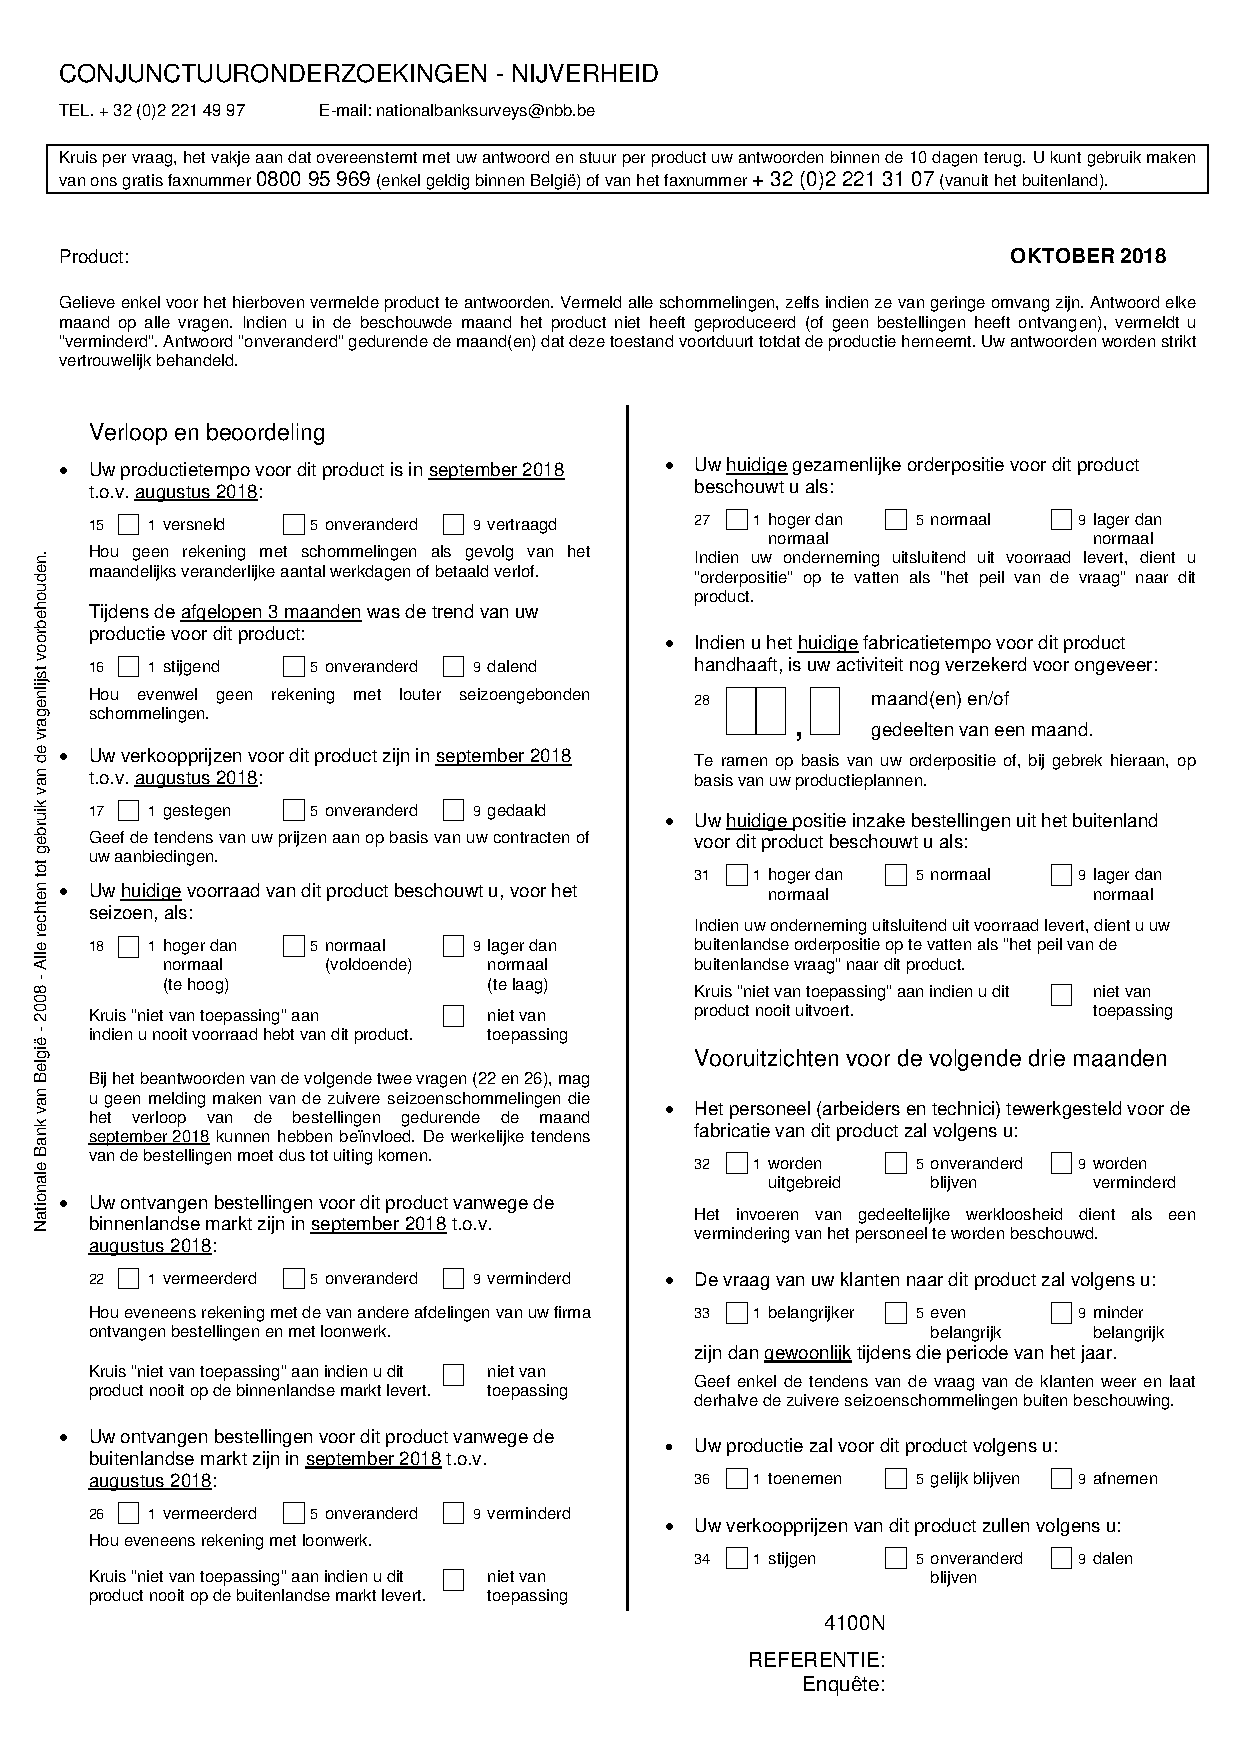
\includegraphics[scale=0.75]{Images/IndustryN.pdf}
    \caption{The Business Survey Questionnaire in Dutch for the Industrial Sector in 2018}
    \label{Questionnaire2018}
\end{figure}

\begin{figure}[H]
    \centering
    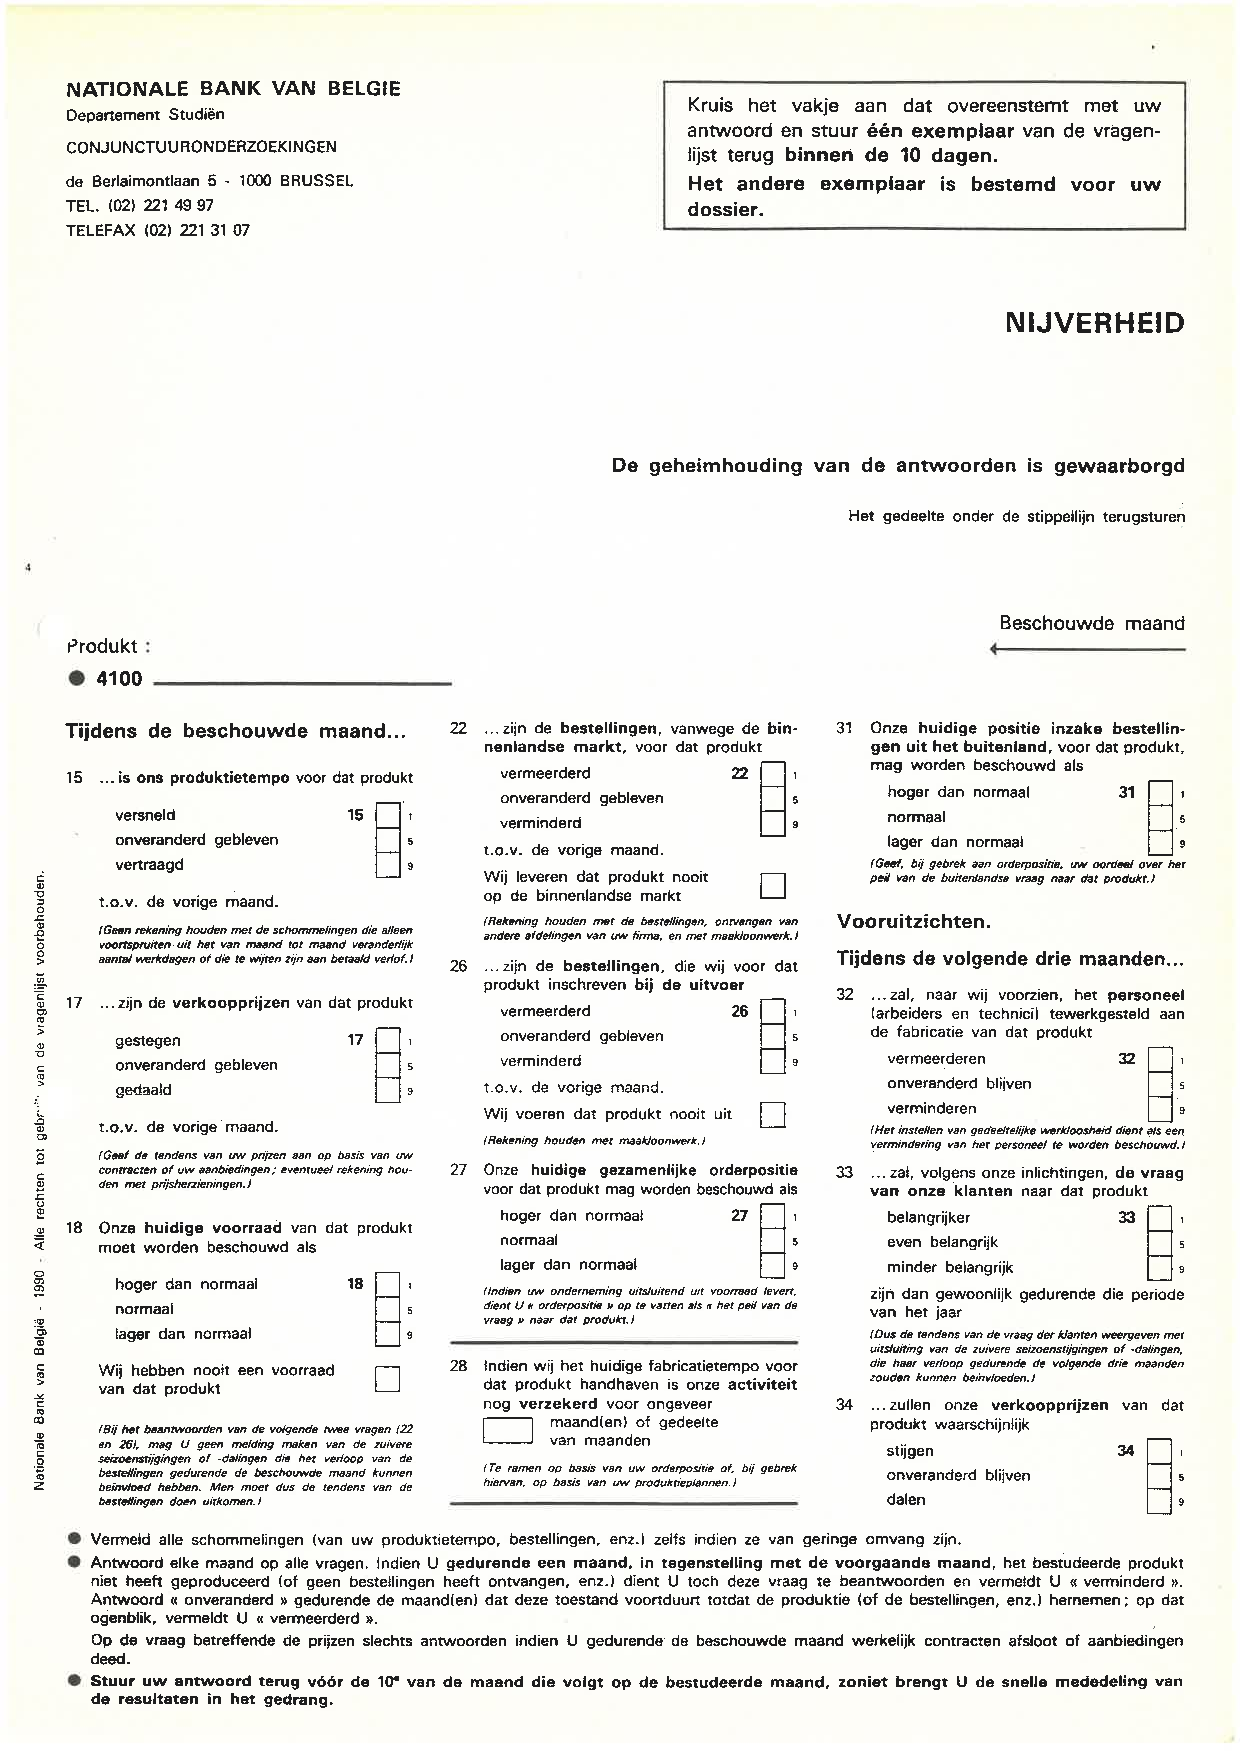
\includegraphics[scale=0.75]{Images/4100N_v1990.pdf}
    \caption{The Business Survey Questionnaire in Dutch for the Industrial Sector in 1990}
    \label{Questionnaire1990}
\end{figure}


\begin{figure}
\begin{subfigure}{.5\textwidth}
  \centering
  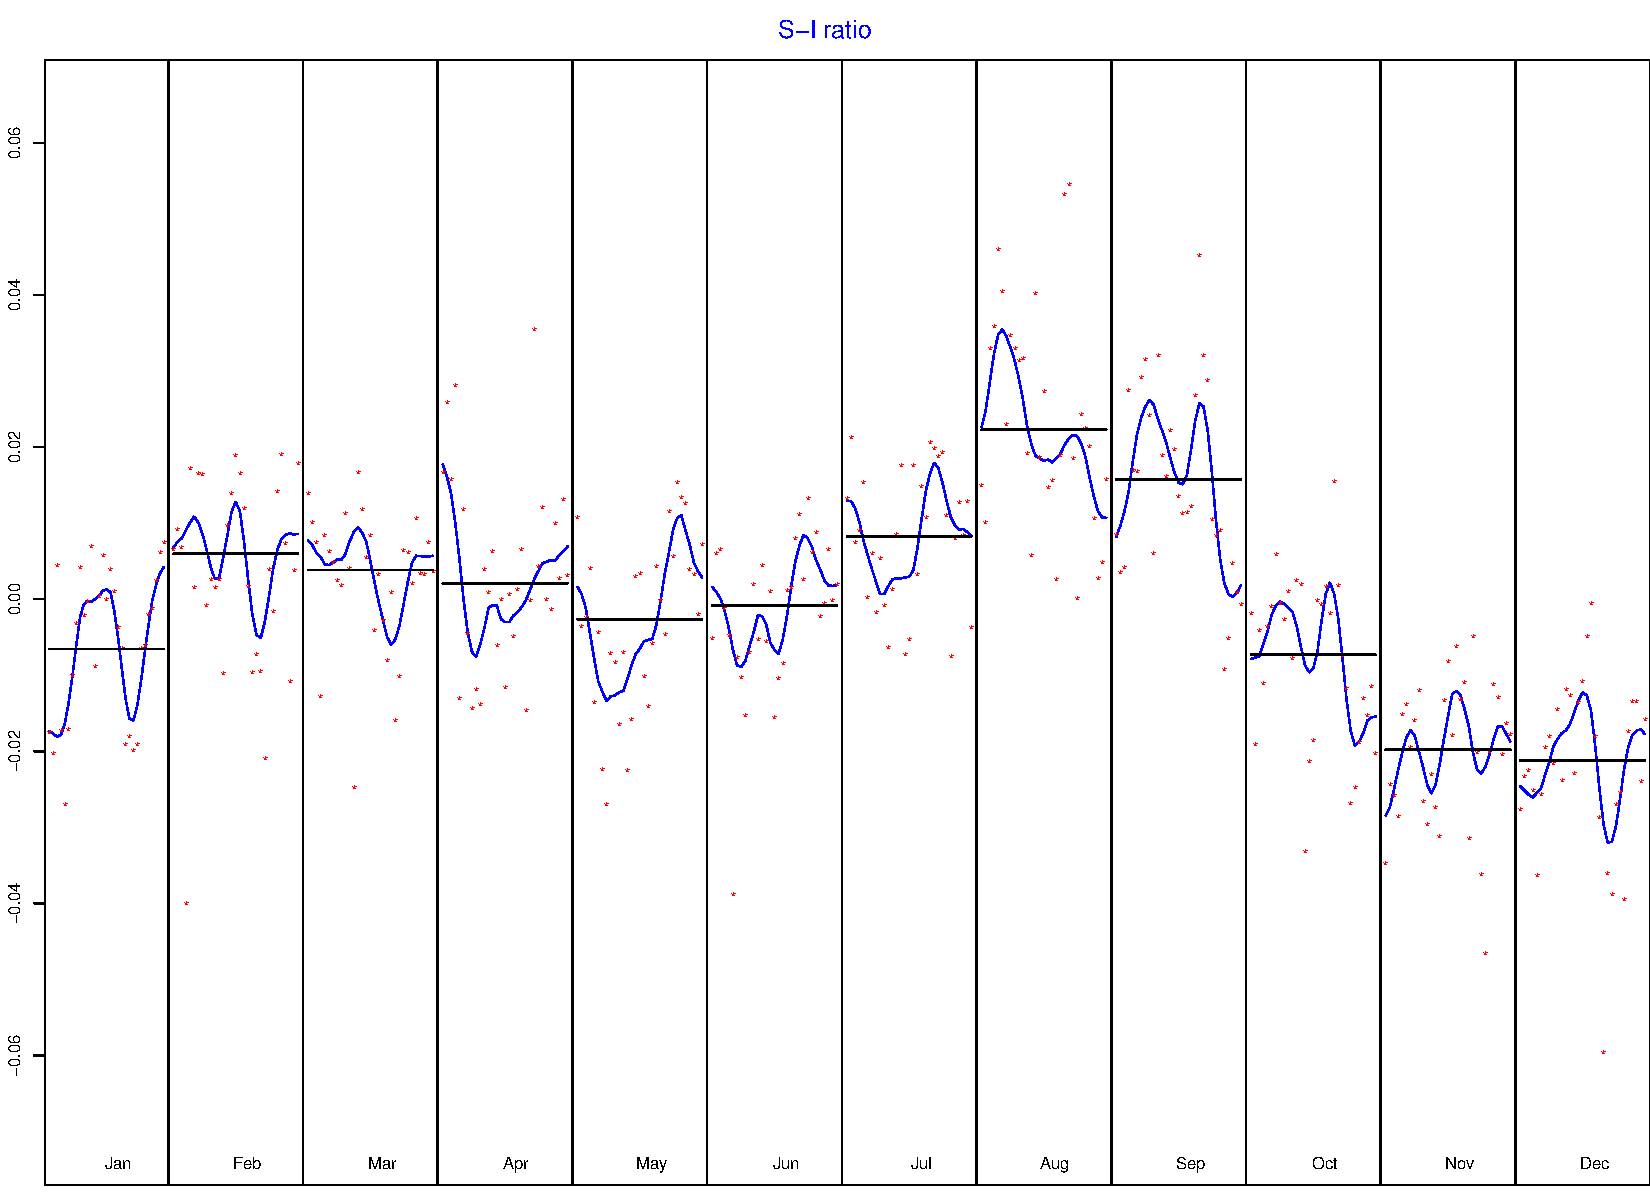
\includegraphics[width=.8\linewidth]{Graphs/S-I_1.pdf}
  \caption{BSI}
\end{subfigure}%
\begin{subfigure}{.5\textwidth}
  \centering
  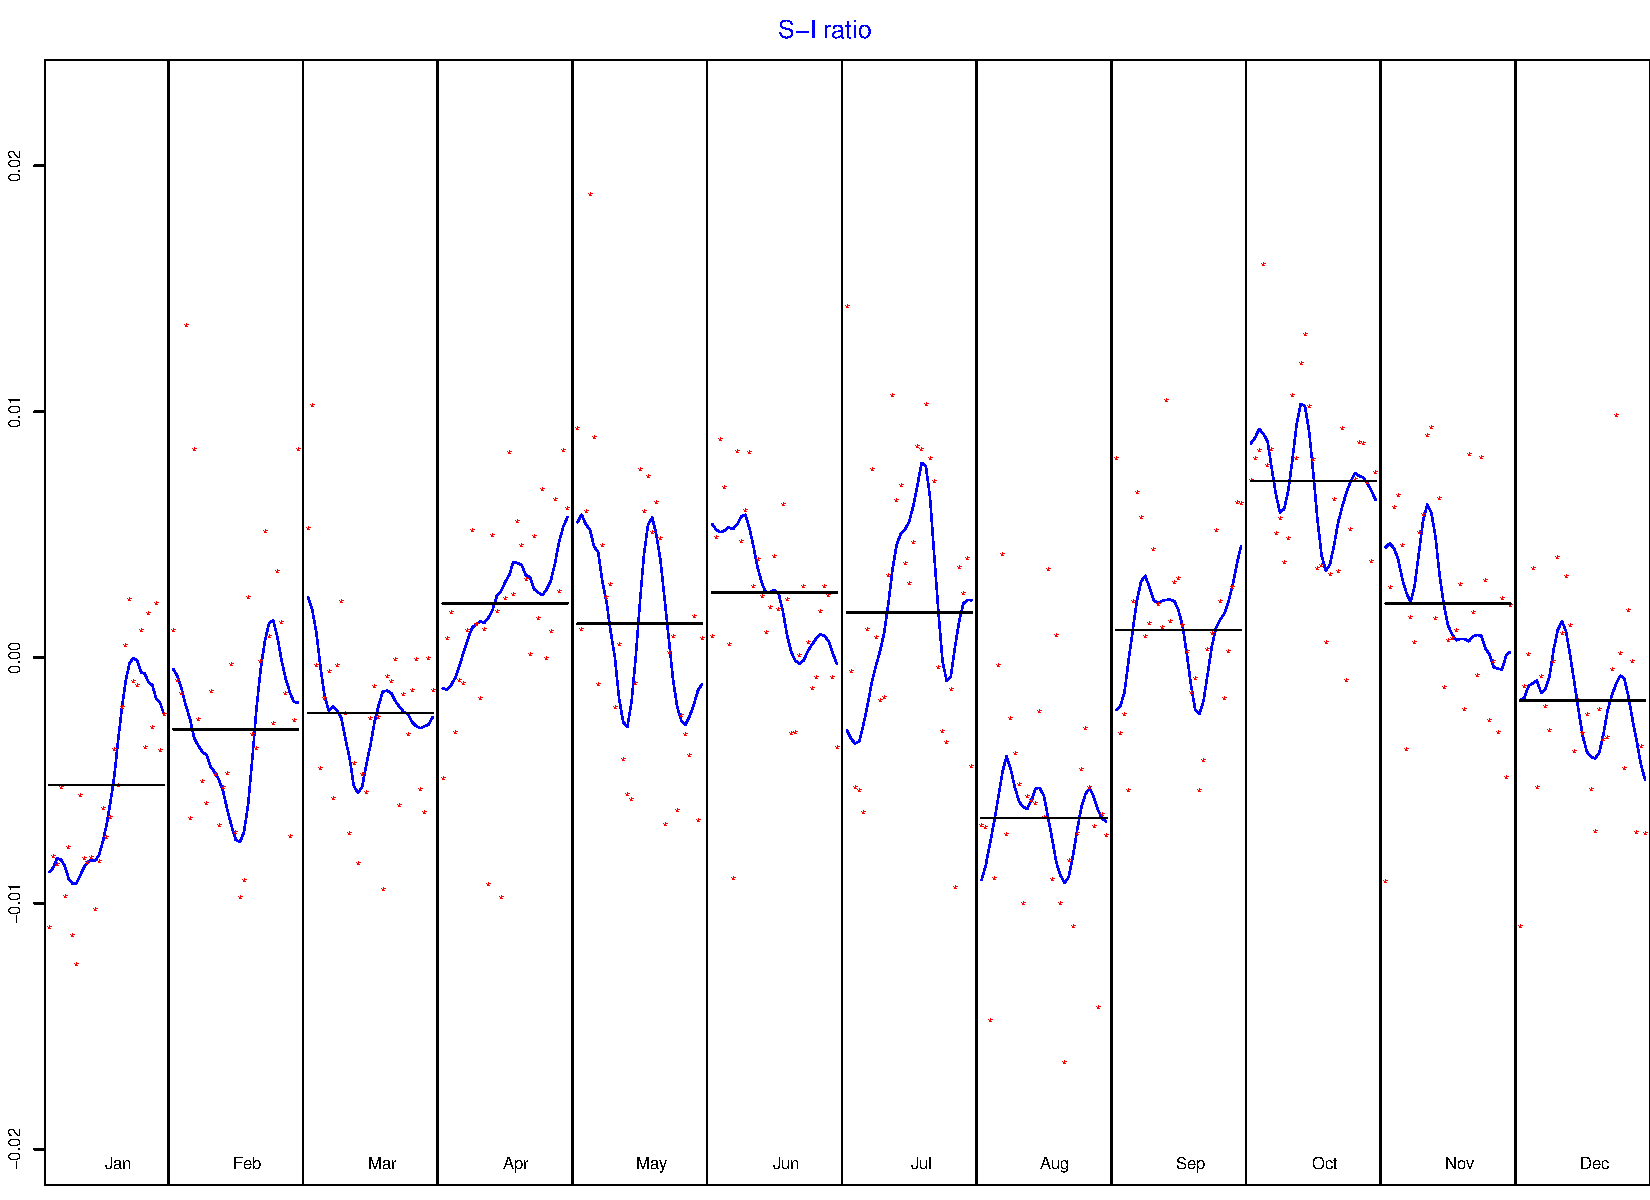
\includegraphics[width=.8\linewidth]{Graphs/S-I_2.pdf}
  \caption{Var(BSI)}
\end{subfigure}
\begin{subfigure}{.5\textwidth}
  \centering
  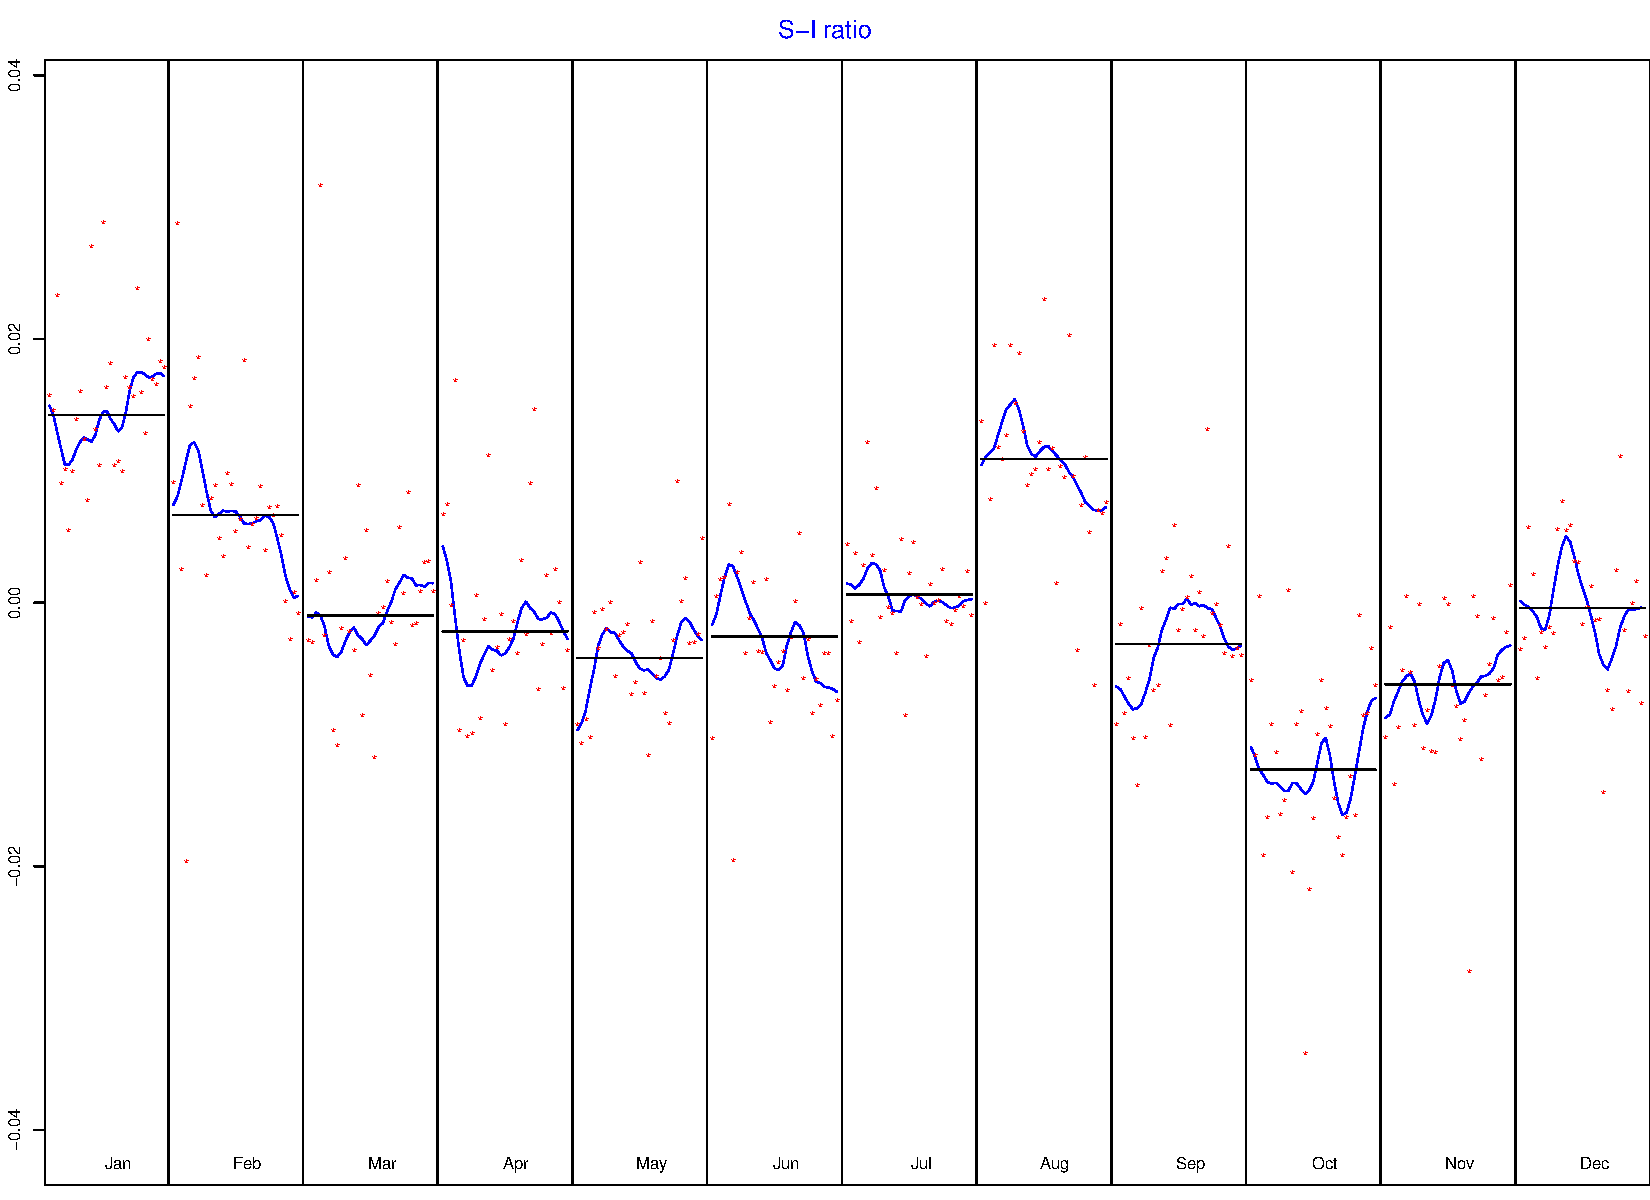
\includegraphics[width=.8\linewidth]{Graphs/S-I_3.pdf}
  \caption{EIR1}
\end{subfigure}
\begin{subfigure}{.5\textwidth}
  \centering
  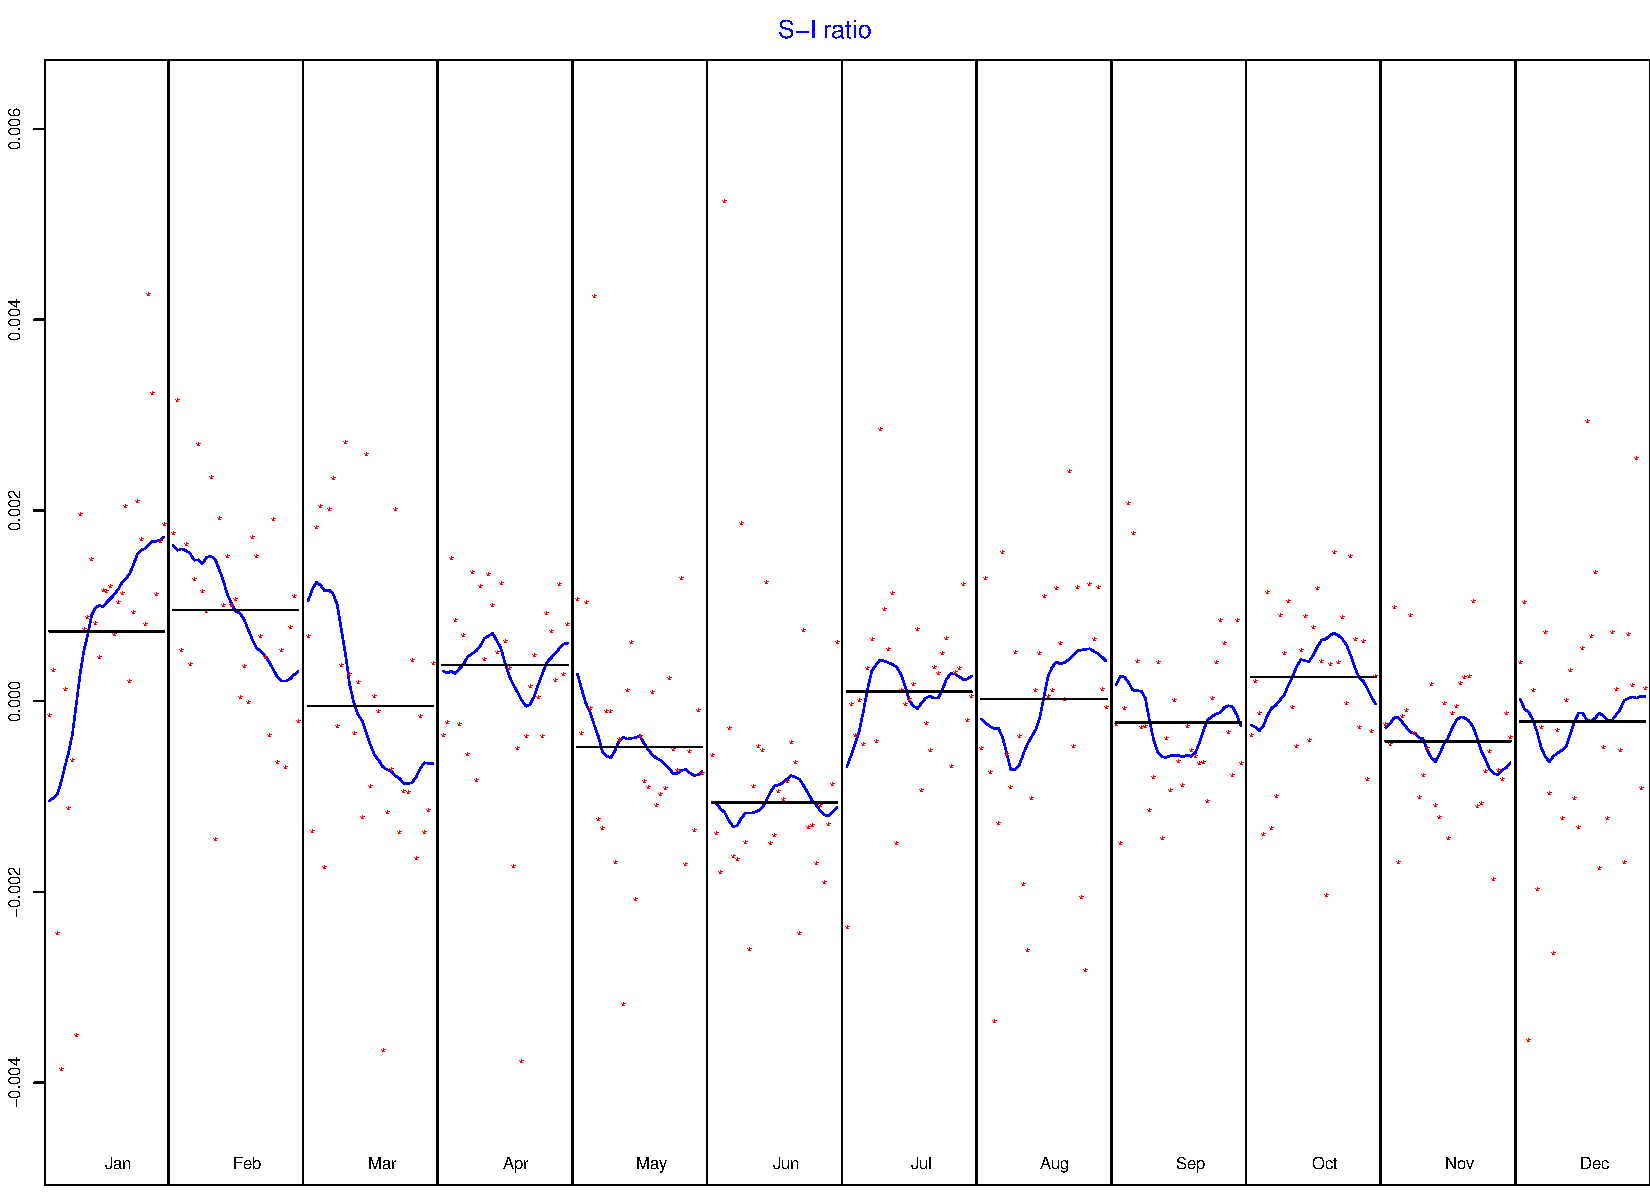
\includegraphics[width=.8\linewidth]{Graphs/S-I_4.pdf}
  \caption{Var(EIR1)}
\end{subfigure}
\begin{subfigure}{.5\textwidth}
  \centering
  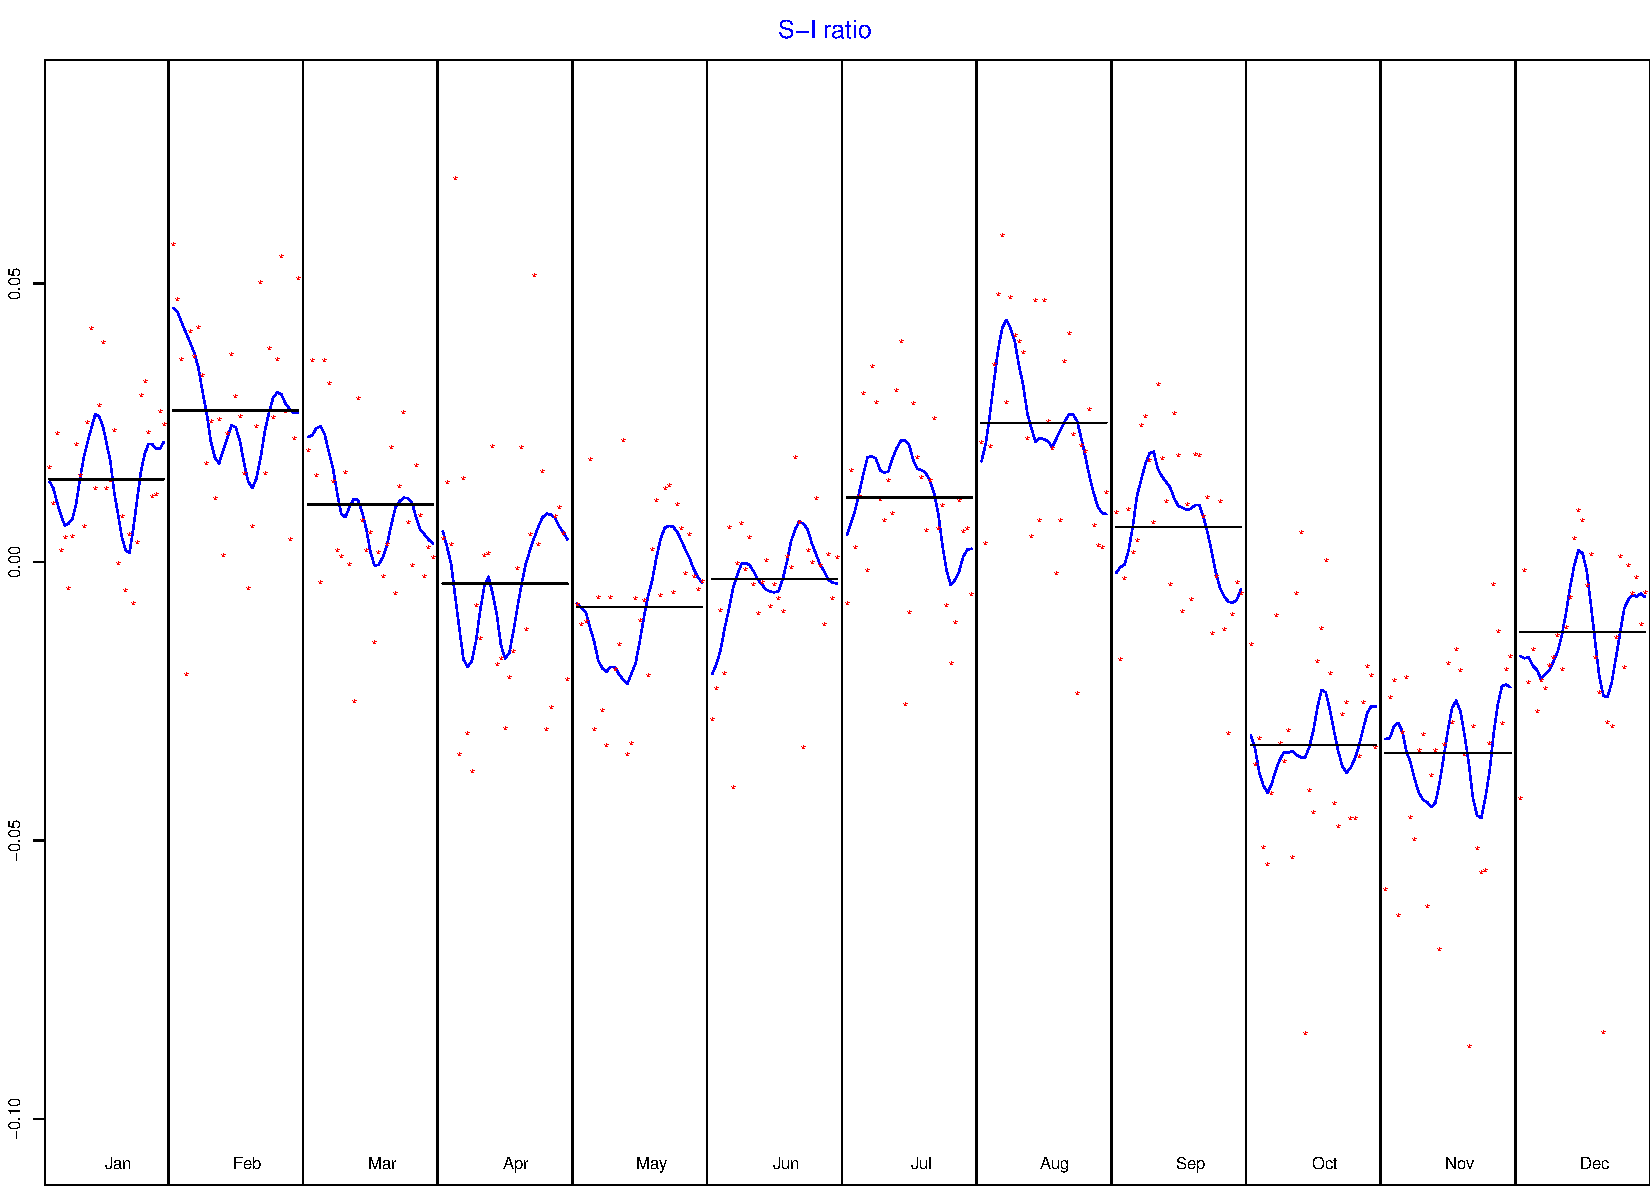
\includegraphics[width=.8\linewidth]{Graphs/S-I_5.pdf}
  \caption{EIR2}
\end{subfigure}
\begin{subfigure}{.5\textwidth}
  \centering
  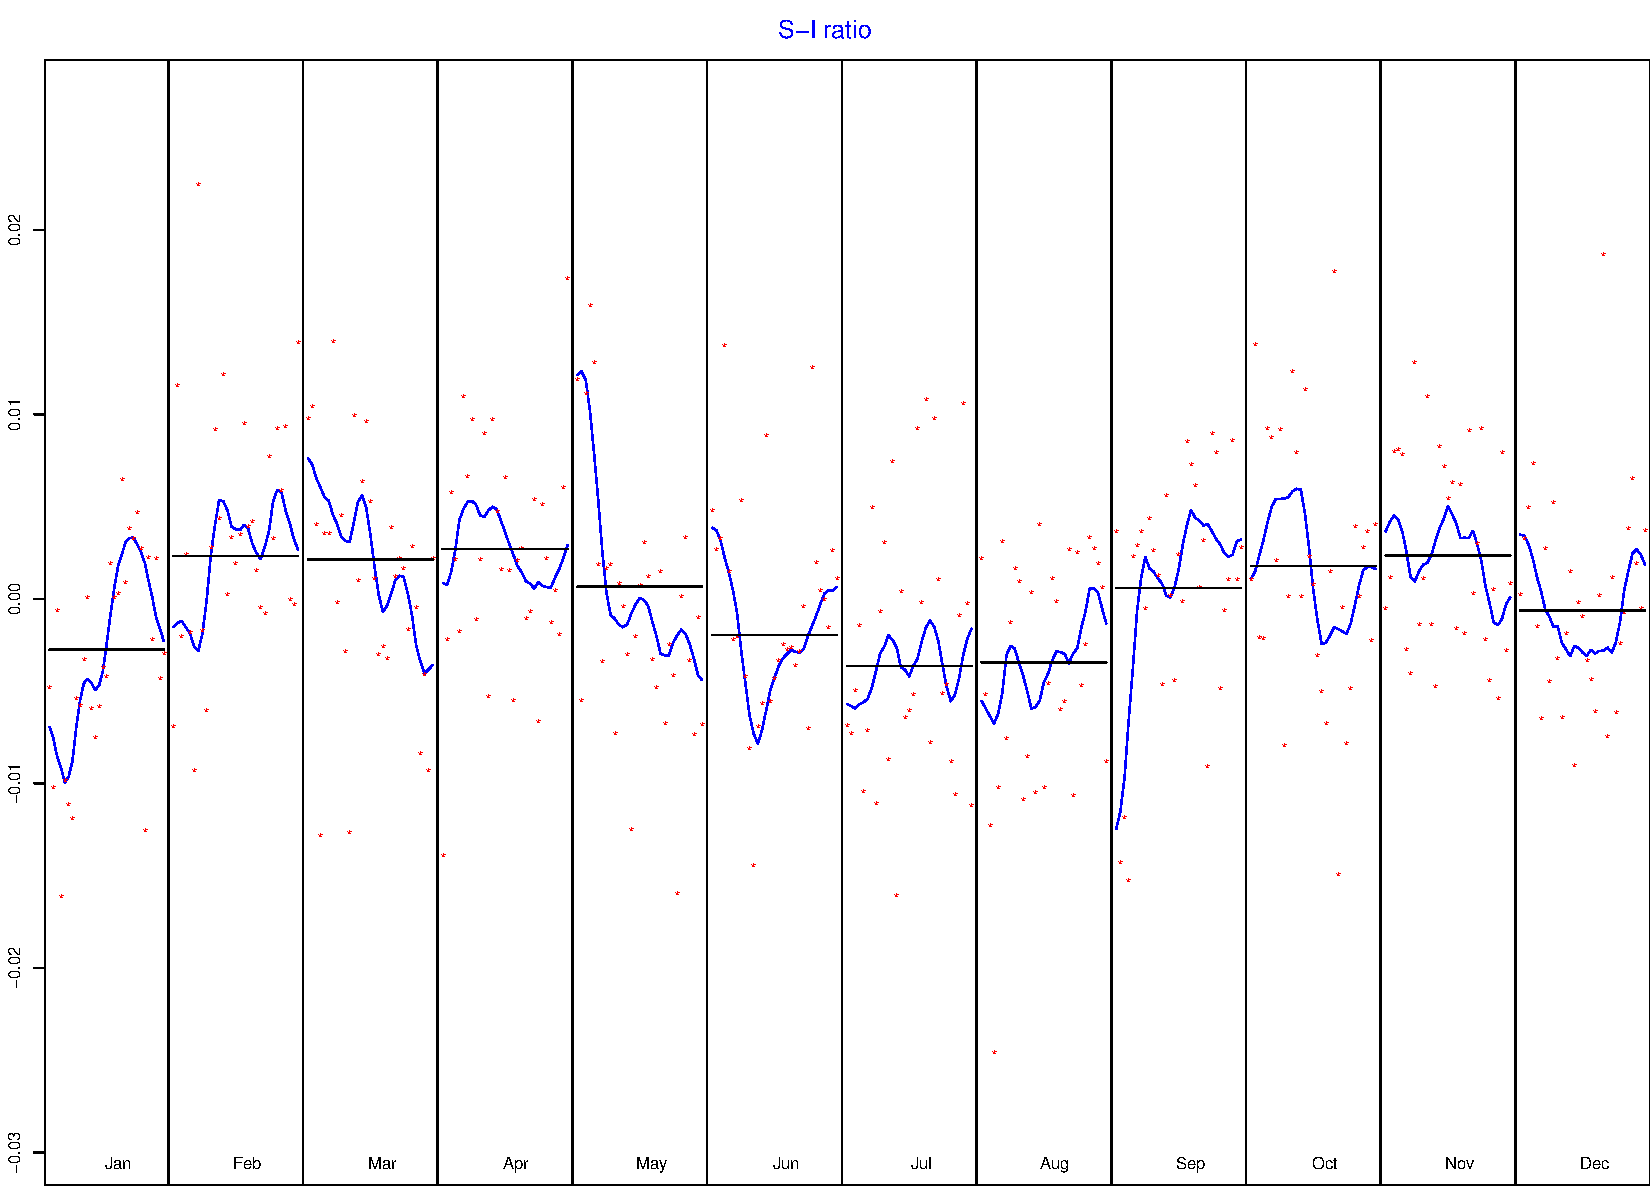
\includegraphics[width=.8\linewidth]{Graphs/S-I_6.pdf}
  \caption{Var(EIR2)}
\end{subfigure}
\begin{subfigure}{.5\textwidth}
  \centering
  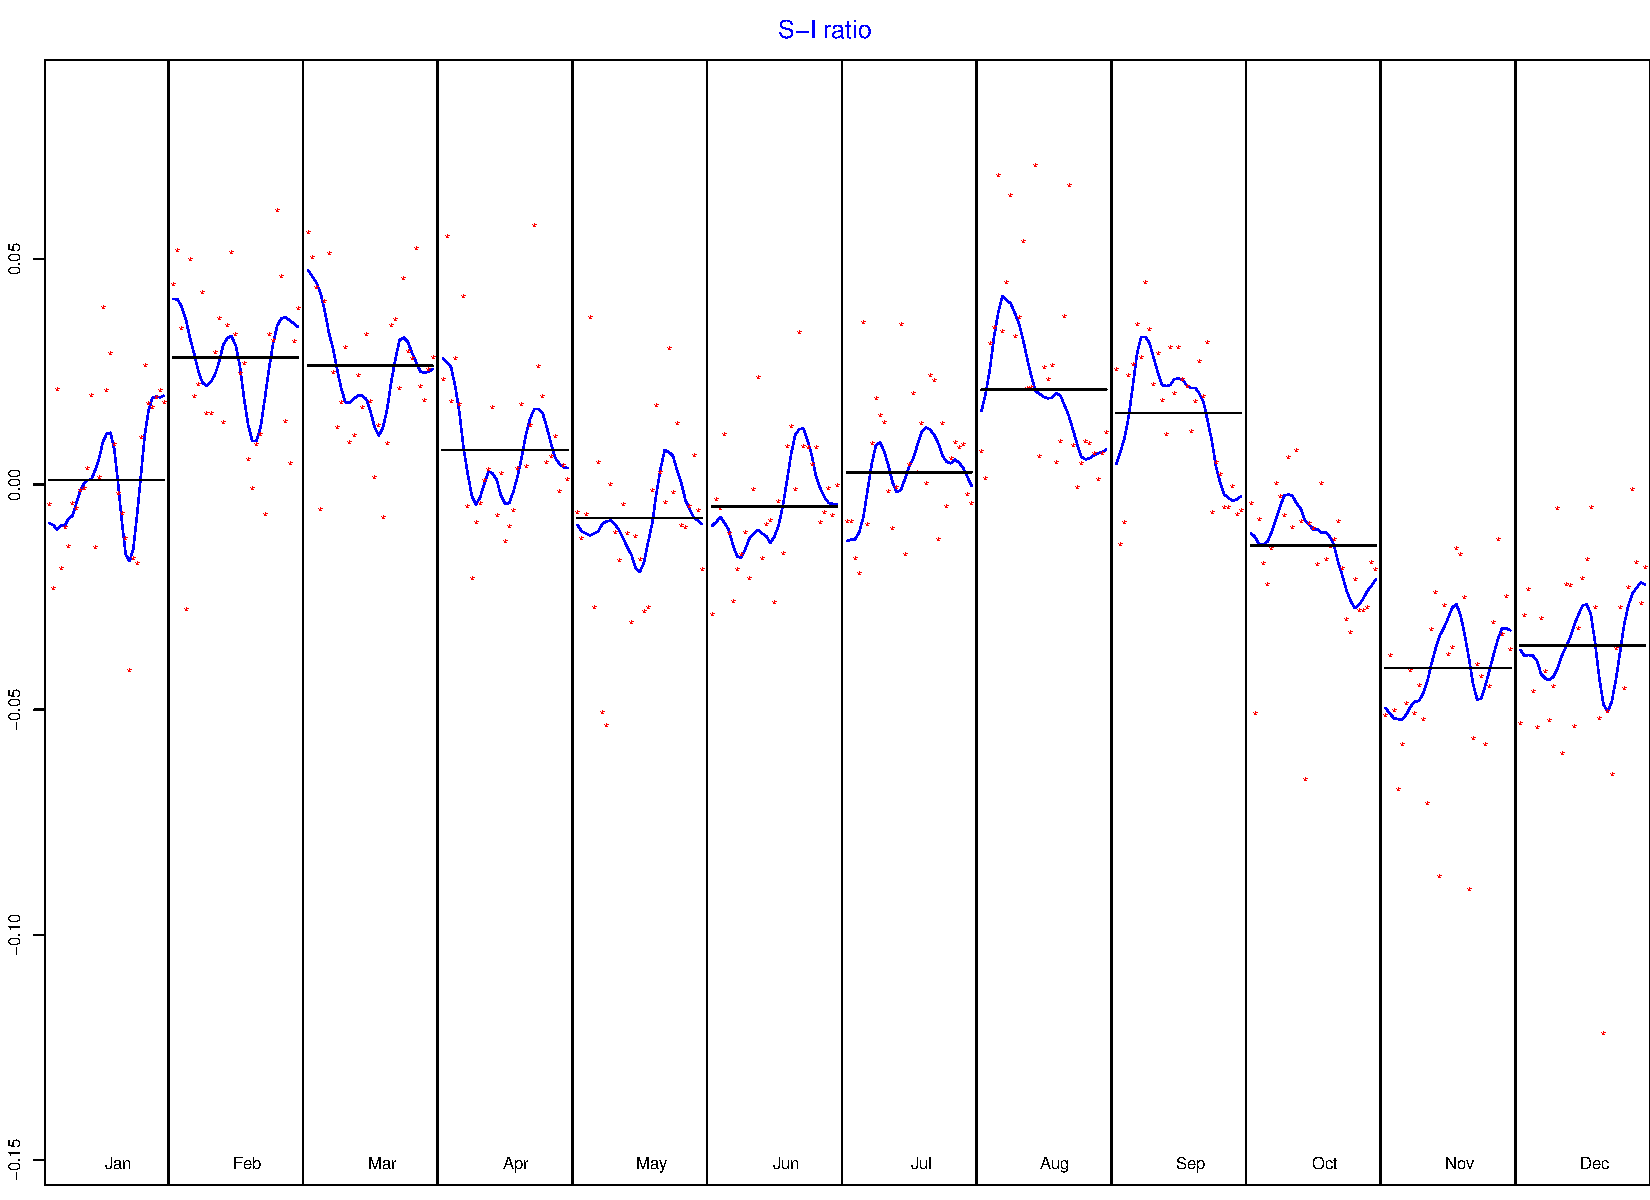
\includegraphics[width=.8\linewidth]{Graphs/S-I_7.pdf}
  \caption{EIR3}
\end{subfigure}
\begin{subfigure}{.5\textwidth}
  \centering
  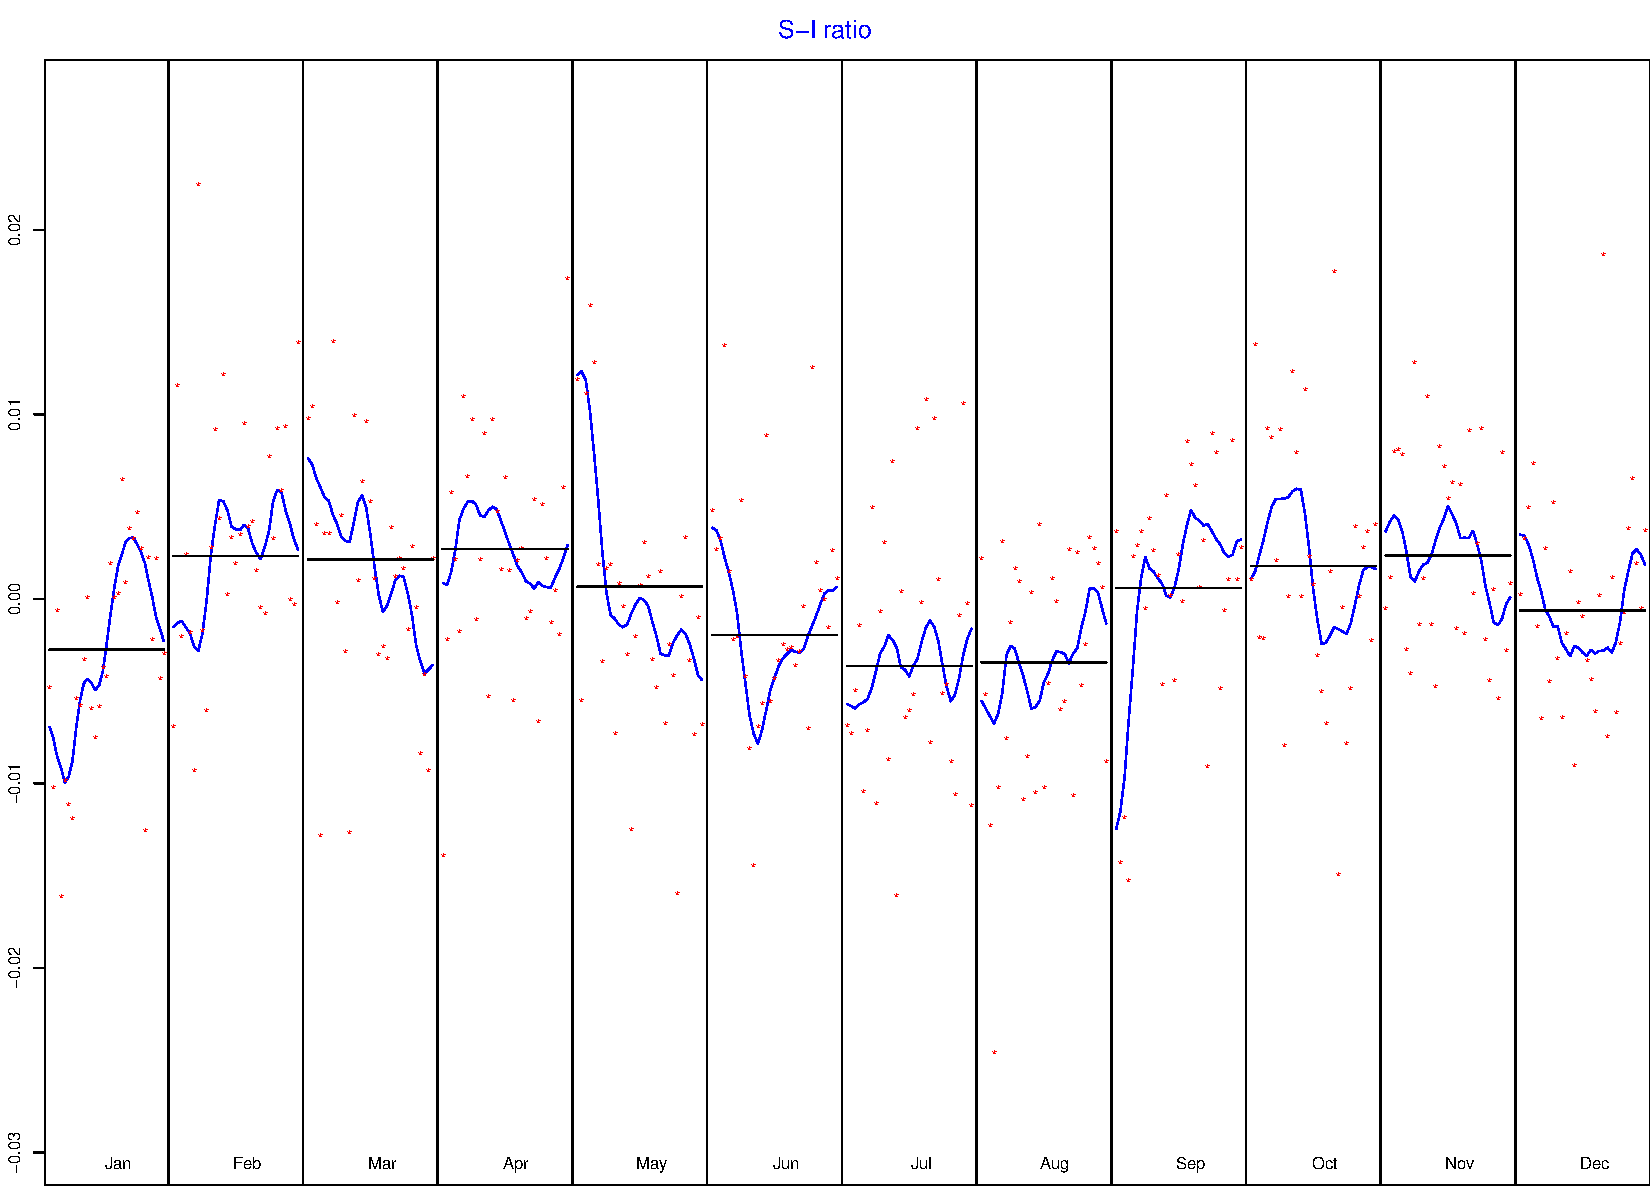
\includegraphics[width=.8\linewidth]{Graphs/S-I_8.pdf}
  \caption{Var(EIR3)}
\end{subfigure}
\caption{S-I plots for the different variables}
\label{fig:S-I seasonal correction RJDemetra}
\end{figure}





\chapter*{Code}
\section*{R code for Seasonal Adjustments}
\href{https://github.com/fabricevb/Master-Thesis/blob/master/R/20Code/Seasonal/20Correction%20model%20data.R}{Link of the R Code for Seasonal Adjustments on https://github.com/fabricevb/Master-Thesis}


\begin{lstlisting}[language=R]
###########################
### Preparing data        #
###########################

Sys.setenv(JAVA_HOME="C:/Program Files/Java/jdk-11.0.3/")

#import libraries
library(rJava)
library(RJDemetra)
library(rjdqa)
library(tidyverse)
library(readxl)
library(xlsx)

# upload data
data <- read_excel("Master-Thesis/Datasets/data.xlsx")

# create time series with the 
data_ts = ts(data, start=c(1988,1), frequency=12)

#################################
# apply seasonal correction X13 #
#################################

# for E(X)
data_E <- data_ts[, "E"]
data_E_model <- x13(data_E, spec="RSA0") # X-13ARIMA method

# for E(Z)
data_EZ <- data_ts[, "Z"]
data_EZ_model <- x13(data_EZ, spec="RSA0") # X-13ARIMA method

# for E(Z2)
data_EZ2 <- data_ts[, "Z2"]
data_EZ2_model <- x13(data_EZ2, spec="RSA0") # X-13ARIMA method

# for E(Z3)
data_EZ3 <- data_ts[, "Z3"]
data_EZ3_model <- x13(data_EZ3, spec="RSA0") # X-13ARIMA method

# for Var(X)
data_Var <- data_ts[, "Var"]
data_Var_model <- x13(data_Var, spec="RSA0") # X-13ARIMA method

# for Var(Z)
data_VarZ <- data_ts[, "Var_Z"]
data_VarZ_model <- x13(data_VarZ, spec="RSA0") # X-13ARIMA method

# for Var(Z2)
data_VarZ2 <- data_ts[, "Var_Z2"]
data_VarZ2_model <- x13(data_VarZ2, spec="RSA0") # X-13ARIMA method

# for Var(Z3)
data_VarZ3 <- data_ts[, "Var_Z3"]
data_VarZ3_model <- x13(data_VarZ3, spec="RSA0") # X-13ARIMA method

data$E_sa <- data_E_model$final$series[, "sa"]
data$Var_sa <- data_Var_model$final$series[, "sa"]
data$Z_sa <- data_EZ_model$final$series[, "sa"]
data$Z2_sa <- data_EZ2_model$final$series[, "sa"]
data$Var_Z_sa <- data_VarZ_model$final$series[, "sa"]
data$Var_Z2_sa <- data_VarZ2_model$final$series[, "sa"]
data$Z3_sa <- data_EZ3_model$final$series[, "sa"]
data$Var_Z3_sa <- data_VarZ3_model$final$series[, "sa"]


################################
# plot seasonal corrected data #
################################

par(mfrow=c(4,2))

# Basic plot with the original series, the trend and the SA series
plot(data_E_model, type_chart = "sa-trend", caption="BSI")
plot(data_Var_model, type_chart = "sa-trend", caption="Var(BSI)")
plot(data_EZ_model, type_chart = "sa-trend", caption="EIR1")
plot(data_VarZ_model, type_chart = "sa-trend", caption="Var(EIR1)")
plot(data_EZ2_model, type_chart = "sa-trend", caption="EIR2")
plot(data_VarZ2_model, type_chart = "sa-trend", caption="Var(EIR2)")
plot(data_EZ3_model, type_chart = "sa-trend", caption="EIR3")
plot(data_VarZ3_model, type_chart = "sa-trend", caption="Var(EIR3)")

par(mfrow=c(1,1))


# look at different results (plots)
# S-I ratio
plot(data_E_model$decomposition)
dev.print(device = pdf, file="S-I_1.pdf", width=11, height=8)
plot(data_Var_model$decomposition)
dev.print(device = pdf, file="S-I_2.pdf", width=11, height=8)
plot(data_EZ_model$decomposition)
dev.print(device = pdf, file="S-I_3.pdf", width=11, height=8)
plot(data_VarZ_model$decomposition)
dev.print(device = pdf, file="S-I_4.pdf", width=11, height=8)
plot(data_EZ2_model$decomposition)
dev.print(device = pdf, file="S-I_5.pdf", width=11, height=8)
plot(data_VarZ2_model$decomposition)
dev.print(device = pdf, file="S-I_6.pdf", width=11, height=8)
plot(data_EZ3_model$decomposition)
dev.print(device = pdf, file="S-I_7.pdf", width=11, height=8)
plot(data_VarZ3_model$decomposition)
dev.print(device = pdf, file="S-I_8.pdf", width=11, height=8)


##########
# OUTPUT #
##########

write.xlsx(data, "Master-Thesis/Datasets/data_sa.xlsx") 
\end{lstlisting}


\newpage
\section*{R code for Correlation Analysis}

\href{https://github.com/fabricevb/Master-Thesis/blob/master/R%20Code/Correlations.R}{Code for the correlation analysis on https://github.com/fabricevb/Master-Thesis}




\section*{R code for Linear (Auto-Regressive) Models}

\href{https://github.com/fabricevb/Master-Thesis/blob/master/R%20Code/Linear%20Regression.R}{Code for Linear Models on https://github.com/fabricevb/Master-Thesis}



\newpage

% ----------------------- Back cover ------------------------------
% Please fill in:
% - Department
% - Department's address
% - Telephone number and fax number
% -----------------------------------------------------------------
\thispagestyle{empty}
\sffamily
%
\begin{textblock}{191}(113,-11)
{\color{blueline}\rule{160pt}{5.5pt}}
\end{textblock}
%
\begin{textblock}{191}(168,-11)
{\color{blueline}\rule{5.5pt}{59pt}}
\end{textblock}
%
\begin{textblock}{183}(-24,-11)
\textblockcolour{}
\flushright
\fontsize{7}{7.5}\selectfont
\textbf{AFDELING}\\
Straat nr bus 0000\\
3000 LEUVEN, BELGI\"{E}\\
tel. + 32 16 00 00 00\\
fax + 32 16 00 00 00\\
www.kuleuven.be\\
\end{textblock}
%
\begin{textblock}{191}(154,-7)
\textblockcolour{}
\includegraphics*[height=16.5truemm]{Images/sedes}
\end{textblock}
%
\begin{textblock}{191}(-20,235)
{\color{bluetitle}\rule{544pt}{55pt}}
\end{textblock}















\end{document}
